%%
%% This is file `ubcsample.tex',
%% generated with the docstrip utility.
%
% The original source files were:
%
% ubcthesis.dtx  (with options: `ubcsampletex')
%% 
%% This file was generated from the ubcthesis package.
%% --------------------------------------------------------------
%% 
%% Copyright (C) 2001
%% Michael McNeil Forbes
%% mforbes@alum.mit.edu
%% 
%% This file may be distributed and/or modified under the
%% conditions of the LaTeX Project Public License, either version 1.2
%% of this license or (at your option) any later version.
%% The latest version of this license is in
%%    http://www.latex-project.org/lppl.txt
%% and version 1.2 or later is part of all distributions of LaTeX
%% version 1999/12/01 or later.
%% 
%% This program is distributed in the hope that it will be useful,
%% but WITHOUT ANY WARRANTY; without even the implied warranty of
%% MERCHANTABILITY or FITNESS FOR A PARTICULAR PURPOSE.  See the
%% LaTeX Project Public License for more details.
%% 
%% This program consists of the files ubcthesis.dtx, ubcthesis.ins, and
%% the sample figures fig.eps and fig.fig.
%% 
%% This file may be modified and used as a base for your thesis without
%% including the licence agreement as long as the content (i.e. textual
%% body) of the file is completely rewritten. You must, however, change
%% the name of the file.
%% 
%% This file may only be distributed together with a copy of this
%% program. You may, however, distribute this program without generated
%% files such as this one.
%% 

% This Sample thesis requires \LaTeX2e
\NeedsTeXFormat{LaTeX2e}[1995/12/01]
\ProvidesFile{ubcsample.tex}[2015/05/31 v1.72 ^^J
 University of British Columbia Sample Thesis]
% This is the \documentclass[]{} command.  The mandatory argument
% specifies the "flavour" of thesis (ubcthesis for UBC).  The
% optional arguments (in []) specify options that affect how the
% thesis is displayed.  Please see the ubcthesis documentation for
% details about the options.
\documentclass[msc,oneside]{ubcthesis}
%
% To compile this sample thesis, issue the following commands:
% latex ubcsample
% bibtex ubcsample
% latex ubcsample
% latex ubcsample
% latex ubcsample
%
% To view use xdvi (on unix systems):
% xdvi ubcsample.dvi
%
% To make a postscript file, use dvips:
% dvips -o ubcsample.ps ubcsample.dvi
%
% To view the postscript file, use ghostview or gv (on unix systems):
% gv ubcsample.ps
%
%************************************************
% Optional packages.
%
% The use of these packages is optional, but they provide various
% tools for more flexible formating.  The sample thesis uses these,
% but if you remove the example code, you should be able to exclude
% these packages.  Only standard packages have been described here;
% they should be installed with any complete LaTeX instalation, but
% if not, you can find them at the Comprehensive TeX Archive Network
% (CTAN): http://www.ctan.org/
%

%******** afterpage ***************************
% This package allows you to issue commands at the end of the current
% page.  A good use for this is to use the command
% \afterpage{\clearpage} right after a figure.  This will cause the
% figure to be inserted on the page following the current one (or on
% the current page if it will fit) but will not break the page in the
% middle.
\usepackage{afterpage}

%******** float *********************************
% This package allows you to customize the style of
% "floats"---floating objects such as figures and tables.  In
% addition, it allows you to define additional floating objects which
% may be included in a list similar to that produces by \listoftables
% and \listoffigures.  Common uses include introducing floats for
% programs and other code bits in Compute Science and Chemical Schema.
\usepackage{float}

%******** tocloft *******************************
% This package allows you to customize and define custom lists such
% as a list of programs or Chemical Scheme.  Note: if you use the
% subfigure package, you must specify that you do as an option here.
% The title option uses the default formatting.  We do not use this
% here as the default formatting is acceptable.  Use the float
% package instead unless you need the extra formatting control
% provided by tocloft.
%\usepackage[subfigure, titles]{tocloft}

%******** alltt *********************************
% The alltt package allows you to include files and have them
% formatted in a verbatim fashion.  This is useful for including
% source code from an additional file.
%\usepackage{alltt}

%******** listings ******************************
% The listings package may be used to include chunks of source code
% and has facilities for pretty-printing many languages.
%\usepackage{listings}

%******** longtable *****************************
% The longtable package allows you to define tables that span
% multiple pages.
\usepackage{longtable}

%******** graphics and graphicx *****************
% This allows you to include encapsulated postscript files.  If you
% don't have this, comment the \includegraphics{} line following the
% comment "%includegraphics" later in this file.
\usepackage{graphicx}

%******** subfigure *****************************
% The subfigure package allows you to include multiple figures and
% captions within a single figure environment.
%\usepackage{subfigure}

%******** here **********************************
% The here package gives you more control over the placement of
% figures and tables.  In particular, you can specify the placement
% "H" which means "Put the figure here" rather than [h] which means
% "I would suggest that you put the figure here if you think it looks
% good."
%\usepackage{here}

%******** pdflscape ********************************
% This allows you to include landscape layout pages by using the
% |landscape| environment.  The use of |pdflscape| is preferred over
% the standard |lscape| package because it automatically rotates the
% page in the pdf file for easier reading.  (Thanks to Joseph Shea
% for pointing this out.)
\usepackage{pdflscape}

%******** natbib ********************************
% This is a very nice package for bibliographies.  It includes options
% for sorting and compressing bibliographic entries.
\usepackage[numbers,sort&compress]{natbib}

%******** psfrag ******************************
% This allows you to replace text in postscript pictures with formated
% latex text.  This allows you to use math in graph labels
% etc. Uncomment the psfrag lines following the "%psfrag" comment
% later in this file if you don't have this package.  The replacements
% will only be visible in the final postscript file: they will be
% listed in the .dvi file but not performed.
\usepackage{psfrag}

%******** hyperref *****************************
% Please read the manual:
% http://www.tug.org/applications/hyperref/manual.html
%
% This adds hyperlinks to your document: with the right viewers (later
% versions of xdvi, acrobat with pdftex, latex2html etc.) this will
% make your equation, figure, citation references etc. hyperlinks so
% that you can click on them.  Also, your table of contents will be
% able to take you to the appropriate sections.  In the viewers that
% support this, the links often appear with an underscore.  This
% underscore will not appear in printed versions.
%
% Note: if you do not use the hypertex option, then the dvips driver
% may be loaded by default.  This will cause the entries in the list
% of figures and list of tables to be on a single line because dvips
% does not deal with hyperlinks on broken lines properly.
%
% NOTE: HYPERREF is sensitive to the ORDER in which it is LOADED.
% For example, it must be loaded AFTER natbib but BEFORE newly
% defined float environments.  See the README file with the hyperref
% for some help with this.  If you have some very obscure errors, try
% first disabling hyperref.  If that fixes the problem, try various
% orderings.
%
% Note also that there is a bug with versions before 2003/11/30
% v6.74m that cause the float package to not function correctly.
% Please ensure you have a current version of this package.  A
% warning will be issued if you leave the date below but do not have
% a current version installed.
%
% Some notes on options: depending on how you build your files, you
% may need to choose the appropriate option (such as [pdftex]) for the
% backend driver (see the hyperref manual for a complete list).  Also,
% the default here is to make links from the page numbers in the table
% of contents and lists of figures etc.  There are other options:
% excluding the [linktocpage] option will make the entire text a
% hyperref, but for some backends will prevent the text from wrapping
% which can look terrible.  There is a [breaklinks=true] option that
% will be set if the backend supports (dvipdfm for example supports
% it but does not work with psfrag.)
%
% Finally, there are many options for choosing the colours of the
% links.  These will be included by default in future versions but
% you should probably consider changing some now for the electronic
% version of your thesis.
\usepackage[unicode=true,
  linktocpage,
  linkbordercolor={0.5 0.5 1},
  citebordercolor={0.5 1 0.5},
  linkcolor=blue]{hyperref}

% If you would like to compile this sample thesis without the
% hyperref package, then you will need to comment out the previous
% \usepackage command and uncomment the following command which will
% put the URL's in a typewriter font but not link them.
%\newcommand\url[1]{\texttt{#1}}

%******** setspace *******************************
% The setspace package allows you to manually set the spacing of the
% file.  UBC may require 1.5 spacing for microfilming of theses.  In
% this case you may obtain this by including this package and issuing
% one of the following commands:
%\usepackage{setspace}
%\singlespacing
%\onehalfspacing
%\doublespacing

\usepackage{enumerate}% http://ctan.org/pkg/enumerate
\usepackage{amssymb}
\usepackage{epstopdf}
\usepackage{wrapfig}
\usepackage{graphicx}
\usepackage[parfill]{parskip}    % Activate to begin paragraphs with an empty line rather than an indent
\usepackage{float}
\usepackage{subcaption}
\usepackage{amsmath}
\usepackage{verbatimbox}
\usepackage[titletoc]{appendix}
\usepackage{setspace}
\usepackage{caption}
\usepackage{url}
\usepackage{braket}
\usepackage{array}
\usepackage{changepage}
\usepackage{mathtools}

\newcolumntype{L}[1]{>{\raggedright\let\newline\\\arraybackslash\hspace{0pt}}m{#1}}

\DeclarePairedDelimiter{\ceil}{\lceil}{\rceil}

% These commands are optional.  The defaults are shown.  You only
% need to include them if you need a different value
\institution{The University Of British Columbia}

% If you are at the Okanagan campus, then you should specify these
% instead.
%\faculty{The College of Graduate Studies}
%\institutionaddress{Okanagan}
\faculty{The Faculty of Graduate and Postdoctoral Studies}
\institutionaddress{Vancouver}

% You can issue as many of these as you have...
\previousdegree{B.Sc., The University of Victoria, 2016}

% You can override the option setting here.
% \degreetitle{Physics}

% These commands are required.
\title{Calibration of SuperCDMS Dark Matter Detectors for Low-Mass WIMPs}
\subtitle{}
\author{Danika MacDonell}
\copyrightyear{2018}
\submitdate{\monthname\ \number\year} % The "\ " is required after
                                      % \monthname to prevent the
                                      % command from eating the space.
\program{Physics}

% These commands are presently not required for UBC theses as the
% advisor's name and title are not presently required anywhere.
%\advisor{Ariel R.~Zhitnitsky}
%\advisortitle{Professor of Physics}

% details of your examining committee
\examiningcommittee{Scott Oser, Physics and Astronomy}{Supervisor}
%\examiningcommittee{Mary Maker, Materials Engineering}%{Supervisory Committee Member}
%\examiningcommittee{Nebulous Name, Department}{Supervisory Committee Member}
\examiningcommittee{Janis McKenna, Physics and Astronomy}{Additional Examiner}

% details of your supervisory committee
%\supervisorycommittee{Ira Crater, Materials Engineering}%{Supervisory Committee Member}
%\supervisorycommittee{Adeline Long, \textsc{CEO} of Aerial Machine Transportation, Inc.}{Supervisory Committee Member}

% One might want to override the format of the section and chapter
% numbers.  This shows you how to do it.  Note that the current
% format is acceptable for submission to the FoGS: If you wish to modify
% these, you should check with the FoGS explicity. prior to making
% the modifications.
\renewcommand\thepart         {\Roman{part}}
\renewcommand\thechapter      {\arabic{chapter}}
\renewcommand\thesection      {\thechapter.\arabic{section}}
\renewcommand\thesubsection   {\thesection.\arabic{subsection}}
\renewcommand\thesubsubsection{\thesubsection.\arabic{subsubsection}}
\renewcommand\theparagraph    {\thesubsubsection.\arabic{paragraph}}
\renewcommand\thesubparagraph {\theparagraph.\arabic{subparagraph}}

\setcounter{tocdepth}{2}
\setcounter{secnumdepth}{2}

% Here is an example of a "Program" environment defined with the
% "float" package.  The list of programs will be stored in the file
% ubcsample.lop and the numbering will start with the chapter
% number.  The style will be "ruled".
\floatstyle{ruled}
\newfloat{Program}{htbp}{lop}[chapter]

% Here is the start of the document.
\begin{document}

%% This starts numbering in Roman numerals as required for the thesis
%% style and is mandatory.
\frontmatter

%%% The order of the following components should be preserved.  The order
%%% listed here is the order currently required by FoGS:        \\
%%% Title (Mandatory)                                           \\
%%% Preface (Mandatory if any collaborator contributions)       \\
%%% Abstract (Mandatory)                                        \\
%%% List of Contents, Tables, Figures, etc. (As appropriate)    \\
%%% Acknowledgements (Optional)                                 \\
%%% Dedication (Optional)                                       \\

\maketitle                      %% Mandatory

\makecommitteepage

\begin{abstract}                %% Mandatory -  maximum 350 words
Observational evidence suggests that the majority of mass in the universe takes the form of non-luminous ``dark matter". The Super Cryogenic Dark Matter Search (SuperCDMS) is a direct-detection dark matter experiment that searches primarily for a well-motivated dark matter candidate known as the weakly-interacting massive particle (WIMP). The experiment looks for an above-background excess of nuclear recoil events in cryogenic solid-state detectors that could be attributed to WIMP-nucleon collisions. The most recent SuperCDMS run at the Soudan underground laboratory set a world-leading limit on the spin-independent WIMP-nucleon cross section for a WIMP mass as low as $\sim$3 GeV/c$^2$, and the next installation of the experiment at SNOLAB aims to be sensitive to WIMP masses below 1 GeV/c$^2$. 

To better understand the response of solid-state germanium detectors to low-mass WIMPs, ``photoneutron" calibration data was taken at the Soudan laboratory in Minnesota by passing quasi-monoenergetic neutrons through SuperCDMS detectors. Gamma rays used in the photoneutron production process create an overwhelmingly dominant background of electron recoil events in the detector. This gamma background is measured directly with regular ``neutron-off" data-taking periods during which the neutron production mechanism is removed. We compare the observed electron and nuclear recoil spectra with Geant4-simulated spectra to obtain a model-dependent calibration of the nuclear recoil energy scale of the detectors. The calibration is performed using a negative log likelihood fit to a parameterized Lindhard ionization yield model. The fit includes a semi-analytical model of the gamma background component obtained from the neutron-off data.

\end{abstract}

\chapter{Lay Summary}

Astronomical observations indicate that the majority of mass in the universe takes the form of ``dark matter". Unlike most of the normal matter that makes up planets and stars, dark matter interacts only very weakly with other matter, and does not produce light. For this reason, it has never been directly detected.  

SuperCDMS is an experiment which seeks to detect dark matter particles by measuring the tiny amounts of vibrational energy that would be produced by a dark matter particle scattering inside a SuperCDMS detector. We present a calibration study which aims to improve our estimate of the masses of dark matter particles that the experiment could measure. We study the relationship between the amount of energy a dark matter particle would give the detector when it scattered -- which is related to its mass -- and the amount of vibrational energy that the detector would actually measure as a result.


\chapter{Preface} % Mandatory if any of the conditions are met

While all discussions in this thesis are my own words, the introductory chapters (Chapters 1-3) exclusively discuss work done by others to motivate the search for dark matter, and describe how SuperCDMS and other experiments perform such a search. 

Chapter 4 presents my contributions to an analysis of calibration data that was taken in 2015 by the SuperCDMS collaboration at the Soudan underground laboratory in Minnesota, U.S.A. The analysis work presented in Chapter 4 was done in close collaboration with an analysis working group within SuperCDMS. As such, the work is heavily reliant upon that of other members of both the analysis group and the wider collaboration, and has benefited from the many ideas and suggestions of my collaborators. I was responsible for developing the data quality cuts, detector resolution model, and ``neutron-off" background model used for the analysis of calibration data taken with detectors operating in CDMSlite mode. I was also responsible for the development and implementation of the unbinned Lindhard yield extraction technique that is applied to the data to obtain an experimental determination of the ionization yield as a function of nuclear recoil energy.

The Lindhard yield extraction technique, and some of the data quality cuts, are built upon early work by Dr. Belina von Krosigk. The high-statistics simulated neutron energy deposition data, produced by Dr. Anthony Villano using his detailed Geant4 simulation of the calibration setup, forms a fundamental input to the Lindhard yield extraction technique. The techniques described in Table 4.1 for defining the phonon pulse shape cuts were developed by Mr. Vijay Iyer.
 

\tableofcontents                %% Mandatory
\listoftables                   %% Mandatory if thesis has tables
\listoffigures                  %% Mandatory if thesis has figures
%\listof{Program}{List of Programs} %% Optional
%% Any other lists should come here, i.e.
%% Abbreviation schemes, definitions, lists of formulae, list of
%% schemes, glossary, list of symbols etc.

\chapter{Acknowledgements}      %% Optional

My supervisor, Scott Oser, has provided constant support and encouragement throughout the past two years. He's taken the time to understand the many stumbling blocks I've encountered while taking my first deep plunge into a data analysis, and his insightful feedback helped me progress from the first simple quality cuts to developing the final `yield extraction' technique. I'm grateful to him for giving me the freedom to follow my work where it took me, providing guidance and much-needed statistics expertise along the way. 

I'm also indebted to Belina von Krosigk for the staggering amount of time she has put into introducing me to the ideas and techniques that have formed the backbone of both my DAQ and analysis work on SuperCDMS, and helping me at every step as I grappled with them. As a result, virtually every aspect of my work has benefited from her support. She is a truly inspiring person to work with, and I can only hope to one day possess some fraction of her calm and humour in the face of panicked masters students who tell her they've just clobbered the DAQ computer. 

I would also like to thank Anthony Villano, Lauren Hsu, and all the other members of photoneutron group whose support, feedback, and ideas have led to many fresh directions, and vastly improved the quality of work in this thesis.

Bill Page has taken a ton of time out of his own graduate work to answer my many questions and help me get acquainted with all things SuperCDMS, for which I am very grateful. 

Last but very much not least, I would like to thank my family for their love and support, and for encouraging me to find what inspires me. 

% Any other unusual prefactory material should come here before the
% main body.

% Now regular page numbering begins.
\mainmatter

% Parts are the largest structural units, but are optional.
%\part{Thesis}

% Chapters are the next main unit.
\chapter{Evidence for Dark Matter}

Observational evidence to date indicates that cold non-baryonic dark matter constitutes $\sim$26\% of all matter and energy in the universe \cite{Planck}, and $\sim$85\% of the total matter content. Despite decades of observational data showing the gravitational effects of dark matter, it has thus far evaded any form of direct experimental detection. As such, its composition and non-gravitational interactions remain a mystery. 

\begin{figure}[H]
\begin{minipage}[c]{0.3\textwidth}
\centering
\caption[Mass and Energy Distribution of the Universe]{Mass and Energy Distribution of the Universe, as derived from the most recent measurements by the Planck collaboration}
\end{minipage}
\begin{minipage}[c]{0.7\textwidth}
\centering
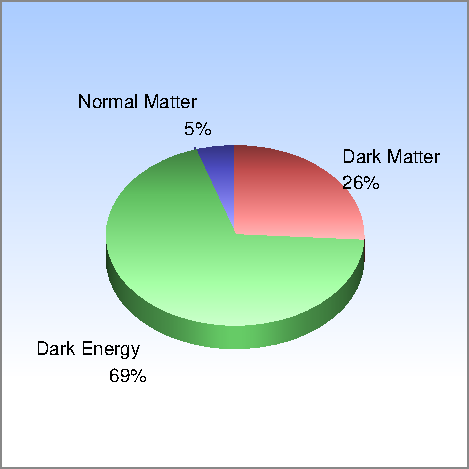
\includegraphics[width=0.7\textwidth]{Figures/Content_PieChart.pdf}
\end{minipage}
\end{figure}

This chapter gives an overview of the experimental evidence for the existence and abundance of non-baryonic dark matter in the universe. The last section discusses the current leading hypotheses predicting the composition of dark matter, focusing primarily on WIMPs, which are the primary search candidate for the Super Cryogenic Dark Matter Search (SuperCDMS). 

\section{Observational Evidence for Dark Matter}

\subsection{Galactic Rotation Curves}

Some of the earliest and clearest evidence for the existence of dark matter in the universe came from studies of galactic rotation curves. In the 1970's, Rubin et al. \cite{Rubin_original, Rubin_SpiralGalaxies} found a strong disagreement between measurements of the rotational speeds of spiral galaxies, and the expectation from Newtonian physics applied to luminosity-based estimates of galactic mass distributions. 

\subsubsection{Expectation from Newtonian Mechanics}

%For an object of mass $m$ rotating at a radius $r$ about the centre of a galaxy, the rotational speed v can be obtained from the gravitational force F$_g=\frac{GMm}{r}$ acting on it from:
%
%\begin{equation}
%\frac{mv^2}{r}=\frac{GM(r)m}{r^2}\implies v(r)=\sqrt{\frac{GM(r)}{r}}
%\end{equation}
%
%where M(r) is the total mass of the galaxy enclosed in a sphere extending to radius r:
%
%\begin{equation}
%M(r)=4\pi\int_0^r\rho(r')r'^2dr'
%\end{equation}

%\begin{figure}[H]
%\begin{minipage}[c]{0.5\textwidth}
%\centering
%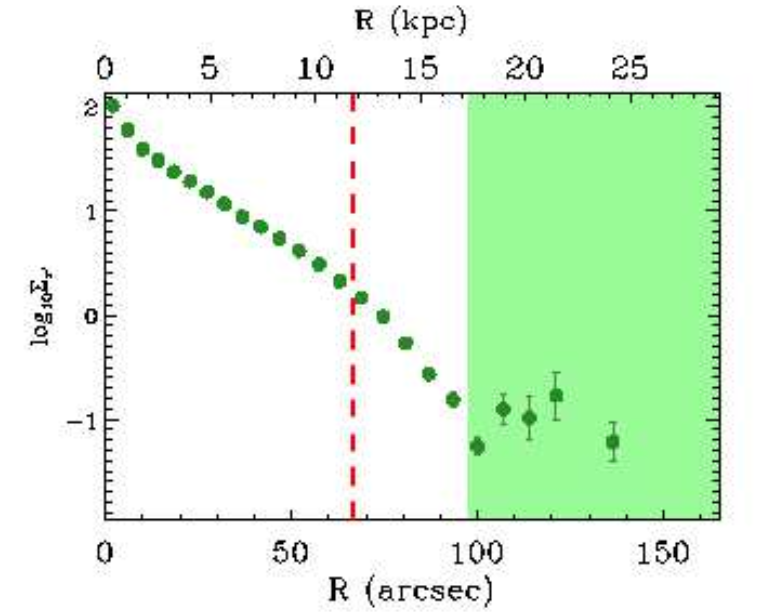
\includegraphics[width=0.95\textwidth]{Figures/UGC_02081.png}
%\subcaption{UGC 02081}
%\end{minipage}
%\begin{minipage}[c]{0.5\textwidth}
%\centering
%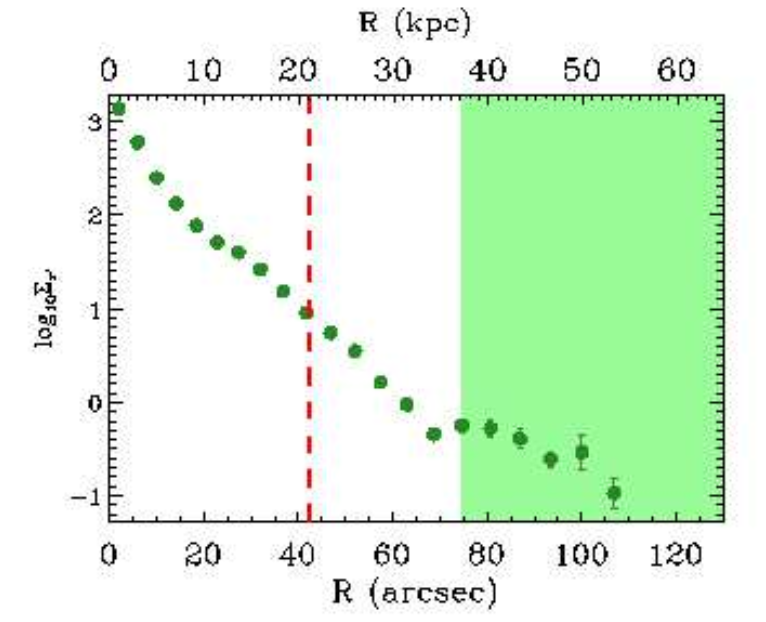
\includegraphics[width=0.95\textwidth]{Figures/UGC_02311.png}
%\subcaption{UGC 02311}
%\end{minipage}
%
%\begin{minipage}[c]{0.5\textwidth}
%\centering
%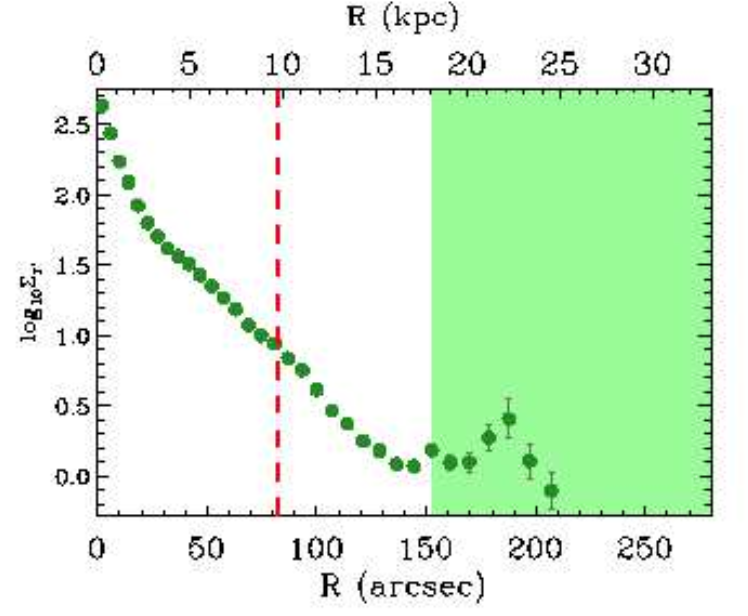
\includegraphics[width=0.95\textwidth]{Figures/NGC_0450.png}
%\subcaption{NGC 0450}
%\end{minipage}
%\begin{minipage}[c]{0.5\textwidth}
%\centering
%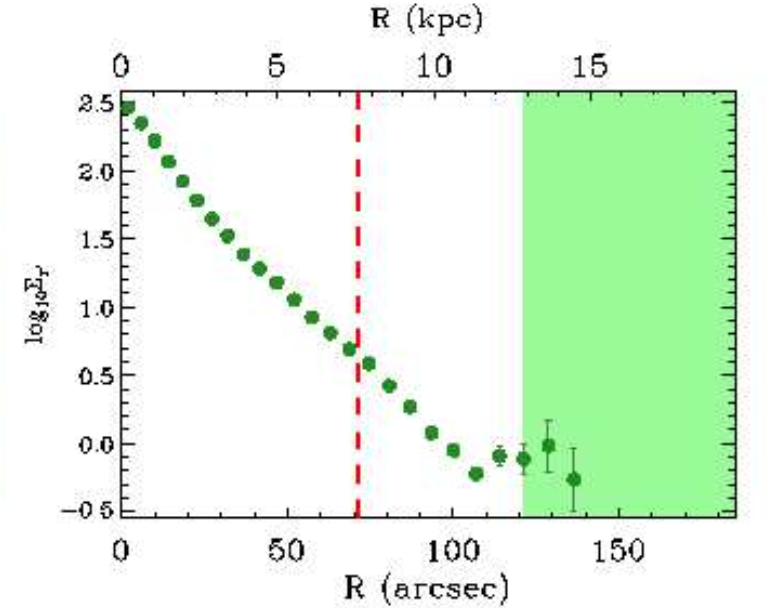
\includegraphics[width=0.95\textwidth]{Figures/NGC_0941.png}
%\subcaption{NGC 0941}
%\end{minipage}
%\caption[Stellar Mass Density Profiles for Sample Spiral Galaxies from SDSS Data]{Stellar mass density profiles for some sample spiral galaxies from Sloan Digital Sky Survey data, calculated from surface density profiles. The y-axis scale is logarithmic. Figures taken from \cite{Stellar_Profiles}.}
%\end{figure}

As early as 1970, it had been observed \cite{Freeman_1970} that the surface brightness distributions of spiral galaxies were comprised of an inner spheroidal component representing the central galaxy bulge, with the surface brightness $I_\text{bulge}(r)$ along the major axis varying with distance $r$ according to:

\begin{equation}
I_\text{bulge}(r)=I_0e^{r^{1/4}}
\end{equation}

and an outer exponential (disk) component with an exponential falloff:

\begin{equation}
I_\text{exp}(r) = I_0e^{-\alpha r}
\end{equation}

Under the assumption that the galactic matter density roughly follows the brightness distribution, the surface density distribution $\mu(r)$ along the major axis of the outer disk would fall off as \cite{Freeman_1970}:

\begin{equation}
\mu_\text{exp}(r) = \mu_0e^{-\alpha r}
\end{equation}

%\begin{figure}[H]
%\centering
%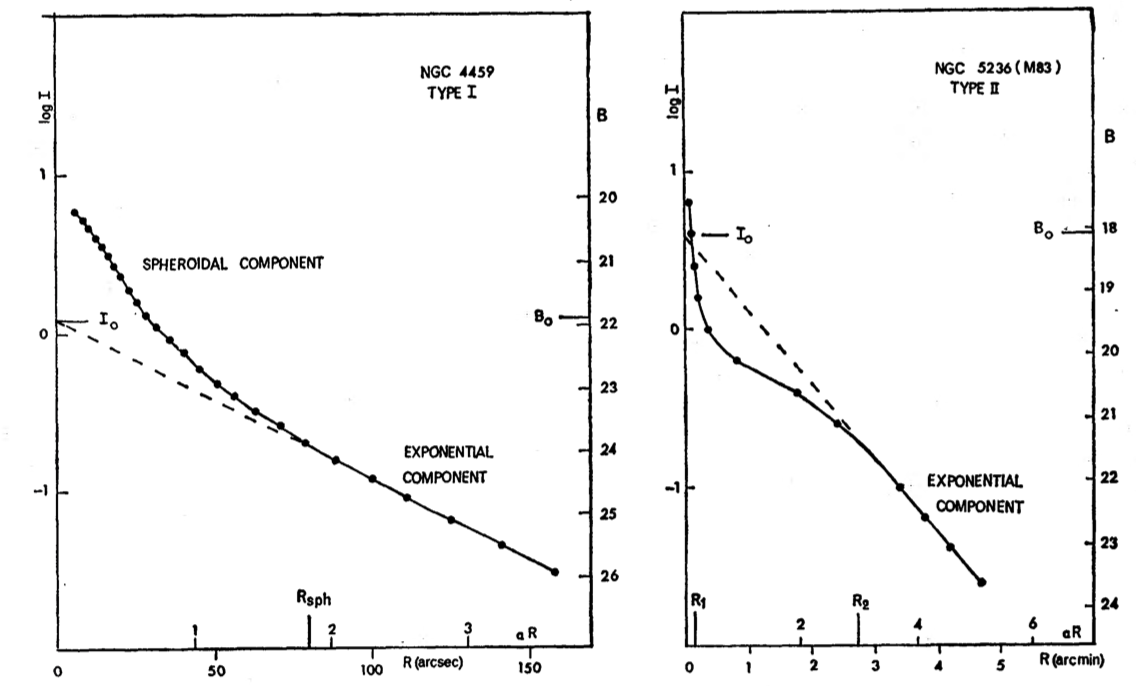
\includegraphics[width=\textwidth]{Figures/Freeman_SurfaceBrightness.png}
%\caption[Surface Brightness Distribution of Spiral Galaxies]{Surface brightness distributions of spiral galaxies, with the inner galaxy bulge modelled by a spheroidal component and the outer disk modelled by an exponential falloff.}
%\end{figure}

Considering only the exponential disk component modelling the luminosity profile far from the galactic bulge, and taking the approximation of a zero-thickness disk with surface density $\mu_\text{exp}(r)$, the rotational speed distribution $v(r)$ along the axis of the exponential disk is calculated in \cite{Freeman_1970} to yield:

\begin{equation}
v^2(r) = \pi r^2 G \mu_0 \alpha\big[I_0(\eta)K_0(\eta) - I_1(\eta)K_1(\eta)\big]
\end{equation}

where $\eta=\frac{1}{2}\alpha r$, $G$ is the gravitational constant, and $I_n$ and $K_n$ are modified Bessel functions. The total mass $\mathcal{M}$ of the disk is $\mathcal{M}=2\pi\mu_0/\alpha^2$. Transforming the radius and rotational speed to the dimensionless forms $\tilde{r}=\alpha r$ and $\tilde{v}=\frac{v}{\sqrt{G\mathcal{M}\alpha}}$, Eq. 1.4 becomes

\begin{equation}
\tilde{v}(\tilde{r}) = \sqrt{\frac{1}{2}\tilde{r}^2\big[I_0(\eta)K_0(\eta) - I_1(\eta)K_1(\eta)\big]}
\end{equation}

Eq. 1.5 is used to plot the expected rotational speed distribution for the exponential disk component, as shown in Fig. 1.2. Under the assumption that the galactic matter density follows the luminosity distribution, the rotational speed should therefore peak, then fall off smoothly beyond the central galaxy bulge. 

\begin{figure}[H]
\centering
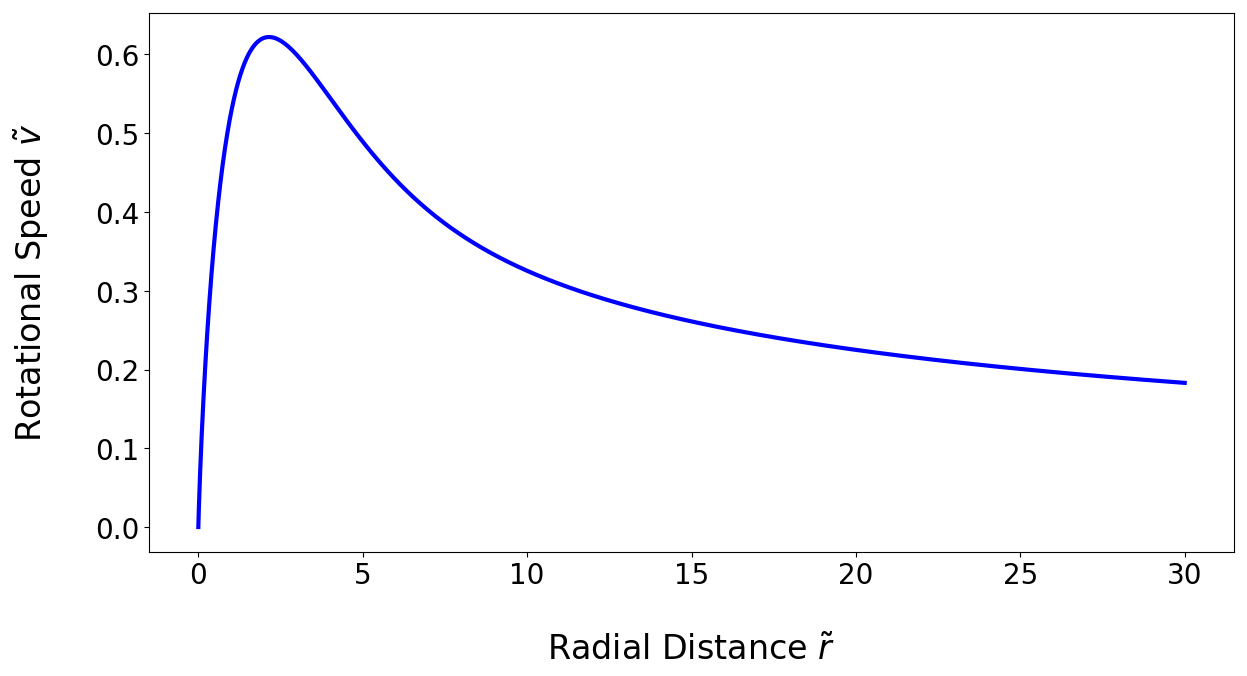
\includegraphics[width=\textwidth]{Figures/Predicted_Rotational_Speeds.png}
\caption[Expected Rotation Speed Distribution of a Spiral Galaxy with an Exponentially-Decaying Mass Density]{Expected dimensionless rotational speed distribution for a spiral galaxy with an exponentially-decaying surface mass density. We expect a peak near $2\tilde{r}$ (see text for definition of $\tilde{r}$), followed by a smooth decay.}
\end{figure}

\subsubsection{Experimental Rotation Curves}

Fig. 1.3 shows a compilation of measured rotational speed distributions for spiral galaxies. Rather than the expected decay at large radii, the mass density increases in the stellar bulge, and then flattens out to radii far beyond the stellar bulge.

\begin{figure}[H]
\centering
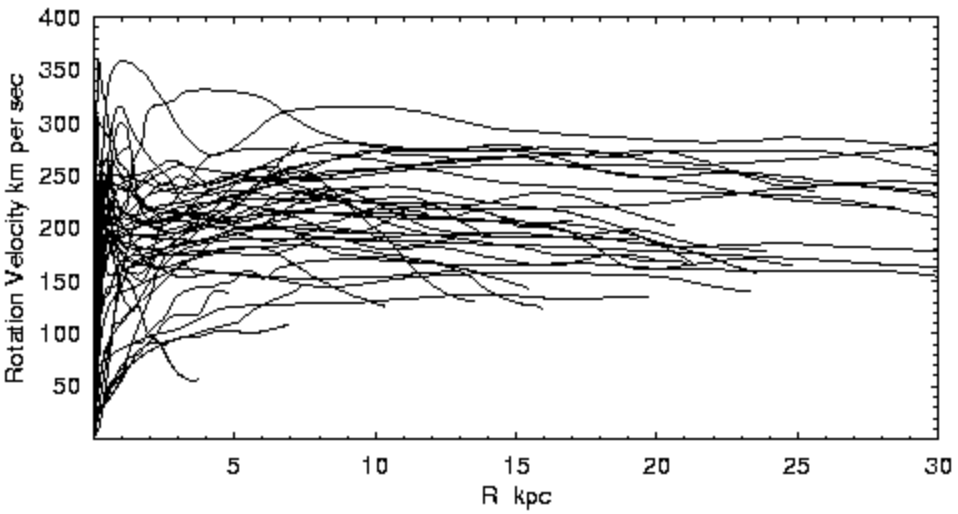
\includegraphics[width=0.7\linewidth]{Figures/Rubin_Rotation.png}
\caption[Measured Rotation Curves of Spiral Galaxies]{Measured rotation curves of spiral galaxies. Figure from $\copyright$ \cite{Rubin_RotationCurves}. Credit: Annual Review of Astronomy and Astrophysics by Annual Reviews. Reproduced with permission of Annual Reviews in the format Thesis/Dissertation via Copyright Clearance Center.}
\end{figure}

%\begin{figure}[H]
%\centering
%\begin{minipage}[c]{0.49\textwidth}
%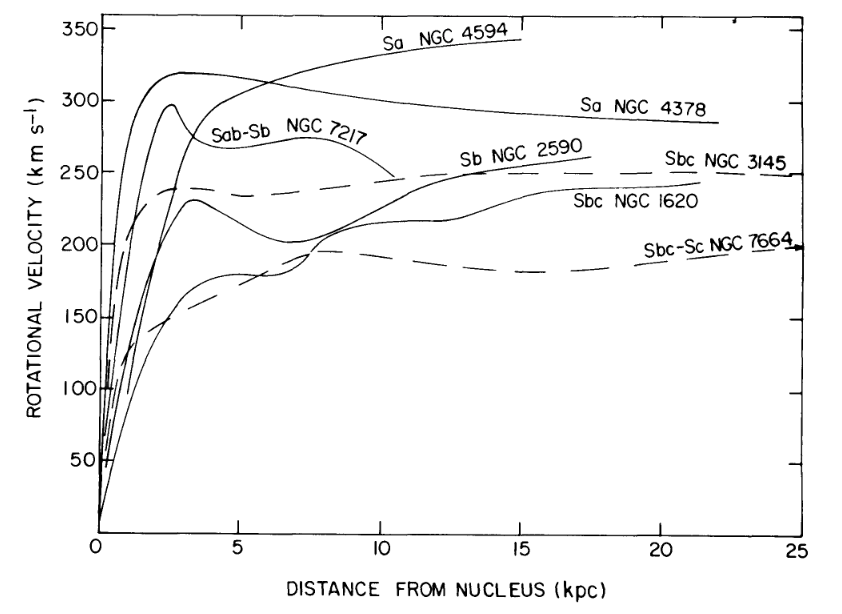
\includegraphics[width=0.95\textwidth]{Figures/Rubin_RotationCurves.png}
%\subcaption{Rotational velocity distributions}
%\end{minipage}
%\begin{minipage}[c]{0.49\textwidth}
%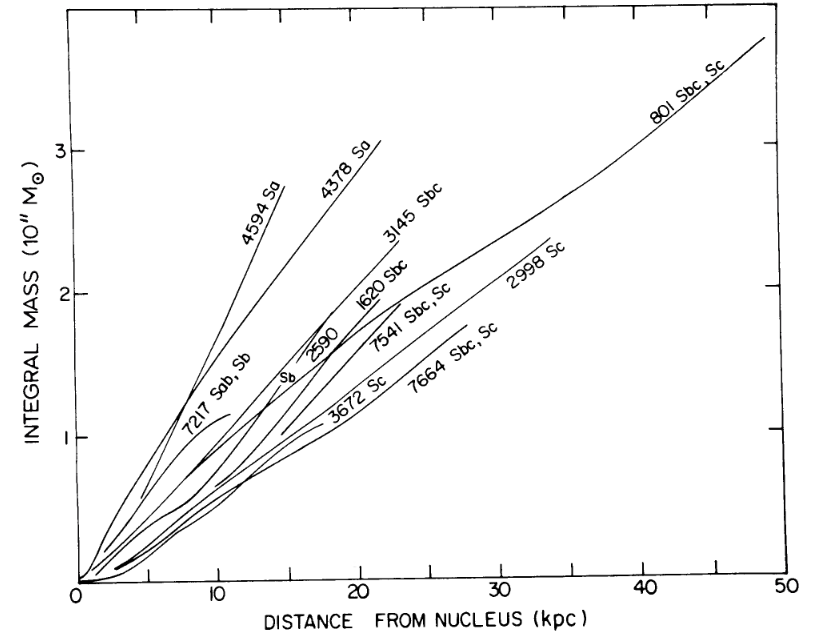
\includegraphics[width=0.95\textwidth]{Figures/Rubin_MassCurves.png}
%\subcaption{Integrated galactic mass distributions}
%\end{minipage}
%\caption[Experimental Rotational Velocity and Integrated Galactic Mass Distributions from Rubin et. al.]{Experimental data for several spiral galaxies studied in \cite{Rubin_SpiralGalaxies}. The left-hand plot shows that, rather than the peak followed by a decay in rotational speeds with distance r from the centre of the galaxy expected from the stellar mass distributions in Fig. 1.2, we instead see the rotational speed flattening out at high radius. The right-hand plot shows that the integrated mass density contained in the spiral galaxies as a function of the radial distance from the centre calculated on the basis of the rotational speed distribution is approximately linear out to high radii.}
%\end{figure}

The constant rotational speeds out to large radii suggest that there must be another form of matter in addition to the luminous matter that is not light-emitting, and whose density falls off much more slowly than the approximately exponential decay of the luminous matter. This non-luminous matter in the galactic halo is identified as ``dark matter". 

\subsection{Collisions of Galaxy Clusters}

A more recent line of evidence pointing to the existence of dark matter in galaxies comes from observations of the distribution of luminous and non-luminous matter following the collision of two galaxy clusters. The Bullet cluster, first investigated by Tucker et. al. in 1995 \cite{Tucker_Bullet} using data from the Chandra NASA X-ray observatory, is the result of such a collision. This merger presents the possibility of decoupling between the luminous and non-luminous (i.e. dark) matter components of the galaxy clusters, thus presenting a unique opportunity to study dark matter in galaxy clusters. 

A study \cite{Bullet_DM} of the Bullet cluster built upon previous work \cite{Allen_GasFrac, Vikhlinin_GasFrac} showing that the mass of hot intracluster plasma in galaxy clusters exceeds the mass of stars comprising galaxies in the cluster by a factor of 3-15. When two clusters collide, it is expected that the relatively sparse stellar components will pass one another with negligible interaction, whereas the fluid-like intracluster plasma will be slowed down due to ram pressure. Therefore, the na$\text{\"i}$ve expectation would be that the majority of matter, and hence gravitational potential, in the cluster merger should reside in the main central component comprised of X-ray emitting intrastellar plasma that has been slowed down by ram pressure, with only the relatively low-mass stellar components at the extreme edges.

A gravitational potential map of the merger was obtained using weak gravitational lensing measurements \cite{Bullet_DM}, which operate on the principle that light is bent by small angles when passing through the gravitational field of the merging galaxy clusters, leading to measurable distortions of galaxies behind the clusters. The resulting deflection causes the images of the galaxies behind the mass in the merger to stretch preferentially in the direction perpendicular to the centre of mass of the cluster, and with enough statistics, the direction and degree of stretching of the galaxies behind the cluster can be used to map out the gravitational potential of the merger.

\begin{figure}[H]
\centering
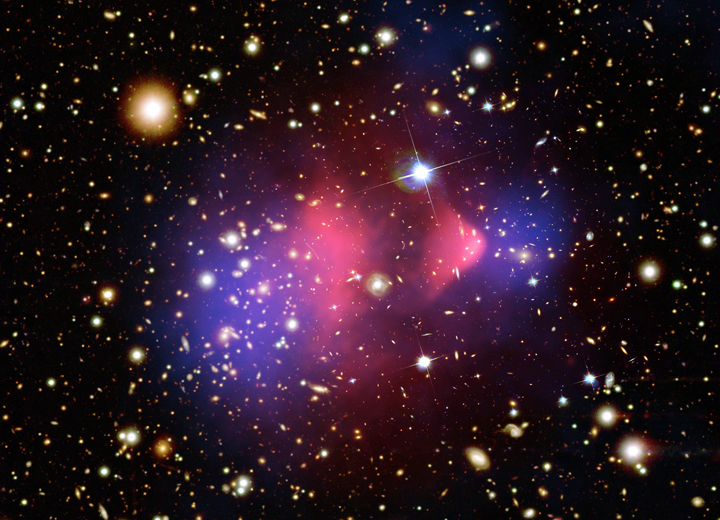
\includegraphics[width=0.6\linewidth]{Figures/Bullet_Cluster.jpg}
\caption[Bullet Cluster Measured by the Chandra X-ray Telescope]{Bullet cluster measured by the Chandra X-ray telescope. Figure reproduced with permission from \cite{CHANDRA}. Credit: X-ray: NASA/CXC/CfA/M.Markevitch et al.; Optical: NASA/STScI; Magellan/U.Arizona/D.Clowe et al.; Lensing Map: NASA/STScI; ESO WFI; Magellan/U.Arizona/D.Clowe et al.}
\end{figure}

In Fig. 1.4, the resulting gravitational potential map (blue) is superimposed on the distribution of X-ray emitting plasma (pink), showing that the vast majority of mass in the cluster merger actually follows the stellar component that passes through effectively unimpeded. This observation provides evidence that the majority of mass in the galaxy clusters is comprised of a non-luminous, gravitationally attractive form of matter that interacts very weakly with both itself and normal matter.

\section{Dark Matter Content of the Universe}

Section 1.1 presented two examples of striking observational evidence for the existence of dark matter in galaxies. However, these examples did little to illuminate the question of exactly how much of the universe is actually composed of dark matter. Nor did they indicate to what extent the dark matter can be accounted for by the normal ``baryonic matter" -- protons, neutrons, and bound electrons -- that constitutes the vast majority of known matter in the universe. 

Of the numerous and diverse observational studies aimed at answering the above questions, the three discussed in this section are intended to loosely reflect the chronology of early findings revealing the need for a dominant non-baryonic dark matter component in the universe, followed by precision measurements of its abundance. Comparison of the present-day measurements of light element abundances with predictions from the theory of Big Bang Nucleosynthesis offered an early estimate of the baryon content of the universe. Studies of galaxy clusters, such as measurements of their gas mass fraction, suggested that the baryon content represents only a sub-dominant fraction of the full matter density of the universe. Recent measurements of anisotropies in the Cosmic Microwave Background (CMB) provide independent confirmation of the dominance of non-baryonic dark matter, with high-precision measurements of the contributions from both baryonic and dark matter to the total mass content of the universe.

\subsection{Cosmological Evolution Model of an Expanding Universe}

This section provides a brief overview of the mathematical formalism that describes the evolution of the universe on the cosmological scale, largely following Chapter 18 of \cite{Hartle}.

\subsubsection{Redshift as a Measure of Relative Speed}

The approaching or recessional speed of luminous objects observed with telescopes -- such as stars, galaxies, and nebulae -- can be estimated by a quantity known as ``redshift" $z$, which is defined as the fractional difference between the wavelength $\lambda_e$ of light emitted at time $t_e$, and its wavelength $\lambda_0$ at time $t_0$ when it arrives at the telescope:

\begin{equation}
z = \frac{\lambda_0-\lambda_e}{\lambda_e}
\end{equation}

The redshift is related to the relative speed $v$ of the light-emitting object via the Doppler effect, which for non-relativistic objects is simply:

\begin{equation}
v=zc
\end{equation}

where $c$ is the speed of light. A positive redshift thus implies that the luminous object is receding away from Earth.


\subsubsection{The Friedmann Equation}

At the cosmological scale, it is found that the universe can be modelled to a good approximation as a homogeneous and isotropic fluid. In 1929, Edwin Hubble demonstrated \cite{Hubble} that the universe is expanding after observing a positive, approximately linear relationship between the redshift -- i.e. recessional speed -- of 24 nebulae, and their independently-measured distance from Earth. In the late 1990's, observational data from Type 1a supernovae was used to further study the expansion of the universe, and these higher-precision measurements revealed \cite{HighZ, SCP} that the universe is expanding at an accelerating rate.  

The entire evolution of the universe, modelled as a homogeneous, isotropic, expanding fluid, is described by a time-dependent scale factor $a(t)$ that quantifies the physical distance between any two points separated by a constant ``coordinate distance". A constant coordinate distance implies that the physical separation distance would remain constant if the universe were not expanding. The time-evolution of the scale factor is described by the Friedmann equation:

\begin{equation}
\dot{a}^2 - \frac{8\pi\rho}{3}a^2 = -k
\end{equation}

where $\rho$ is the total energy density of the universe, and $k$ is a constant that quantifies the overall spacetime curvature of the universe: $k=0$ implies that spacetime is flat on cosmological scales, $k=+1$ implies a closed universe with positive curvature, and $k=-1$ implies an open universe with negative curvature.  The existing astronomical evidence, most recently from the Planck mission \cite{Planck}, is strongly in favour of a flat universe ($k=0$).

\subsubsection{Dimensionless Energy Density}

Solving for the energy density $\rho$ in the Friedmann equation (Eq. 1.8) yields:

\begin{equation}
\rho = \frac{3}{8\pi}\frac{\dot{a}^2+k}{a^2}
\end{equation}

Setting $k=0$, corresponding to a flat universe, and evaluating Eq. 1.9 at the present time $t_0$ yields what is called the ``critical energy density" $\rho_\text{crit}$:

\begin{equation}
\rho_\text{crit} = \frac{3}{8\pi}\Bigg(\frac{\dot{a}(t_0)}{a(t_0)}\Bigg)^2 = \frac{3}{8\pi}H_0^2
\end{equation}

where $H_0\equiv\frac{\dot{a}(t_0)}{a(t_0)}$ is the Hubble constant, which gives a measure of the rate of expansion of the universe at the present time. The most recent measurement of $H_0$ by the Planck mission \cite{Planck} yields a value of 66.26$\pm$0.98 km s$^{-1}$ Mpc$^{-1}$.

It is common to express the energy density $\rho_X$ of a particular component X of the universe's energy budget in terms of the critical energy density as:

\begin{equation}
\Omega_X = \frac{\rho_X}{\rho_\text{crit}}
\end{equation}

With this notation, the sum $\Omega=\sum_n\Omega_n$ over all contributions to the energy density in the universe will be $\Omega$=1 for a flat universe, $\Omega<1$ for an open universe ($k=-1$), and $\Omega>1$ for a closed universe ($k=+1$). Under the assumption of a flat universe, the energy density $\Omega_X$ thus represents the fractional contribution of component X to the combined energy density of the universe. This quantity is often reported with an additional factor of $h^2\equiv\big(\frac{H_0}{100\text{ km s}^{-1}\text{ Mpc}^{-1}}\big)^2$.

 \subsection{Big Bang Nucleosynthesis}
 
Big Bang Nucleosynthesis (BBN) is believed to have taken place during the first $\sim100$s to 20 minutes \cite{BBN_Probe, BBN_PDG} after the Big Bang, as the temperature of the early universe cooled sufficiently to allow the formation of light elements. This process of nucleon production continued until the temperature and density of the expanding universe became too low for these nuclear reactions to occur \cite{BBN_2017}. 

BBN produced what is known as the ``primordial abundance" of $^2$H (also known as D), $^3$H, $^3$He, $^4$He, and $^7$Li. The abundances of these light elements are typically expressed in terms of their number density $n$ relative to the H abundance (eg. $\text{D}/\text{H}\equiv n(\text{D})/n(\text{H}$)), with the exception of $^4$He, which is expressed in terms of its mass density relative to the total baryon mass density: $Y\equiv\rho({^4\text{He}})/\rho_{b}$. Once stars began to form, the nuclear fusion reactions between atoms within stars, known as ``stellar nucleosynthesis", became the dominant process capable of altering these primordial abundances \cite{BBN_Probe}. The theory of BBN provided the earliest estimate of the baryon contribution $\Omega_b$ to the energy density of the universe \cite{BBN_Probe}, which has only recently been overcome in sensitivity by detailed studies of the CMB, discussed in Section 1.2.4. 

The rate of fusion reactions taking place during BBN is predicted to increase with the density $n_b$ of baryons in the universe at the time. The baryon number density is typically normalized by the photon number density $n_\gamma$ to obtain the baryon-to-photon ratio $\eta$ \cite{BBN_2017}:

\begin{equation}
\eta = \frac{n_b}{n_\gamma}
\end{equation}

BBN theory
%, which is based on well-established Standard Model physics \cite{BBN_PDG}, 
predicts the variation in the primordial abundances of D/H, $^3$He/H, and $^7$Li/H, and to a small degree $Y=\rho(^4\text{He})/\rho_b$, with the present-day $\eta$, as shown in Fig. 1.5. As such, the theory may be applied to present-day measurements of the primordial abundances of these light elements to obtain an experimental estimate of $\eta$. The results obtained from the different light element abundances can also be compared for consistency. The measured value of $\eta$ is combined with measurements of H$_0$, and of $n_\gamma$ deduced from the present-day CMB temperature, to estimate the baryon density $\Omega_b$ of the universe using Equations 1.10-1.12. 

\begin{figure}[H]
\centering
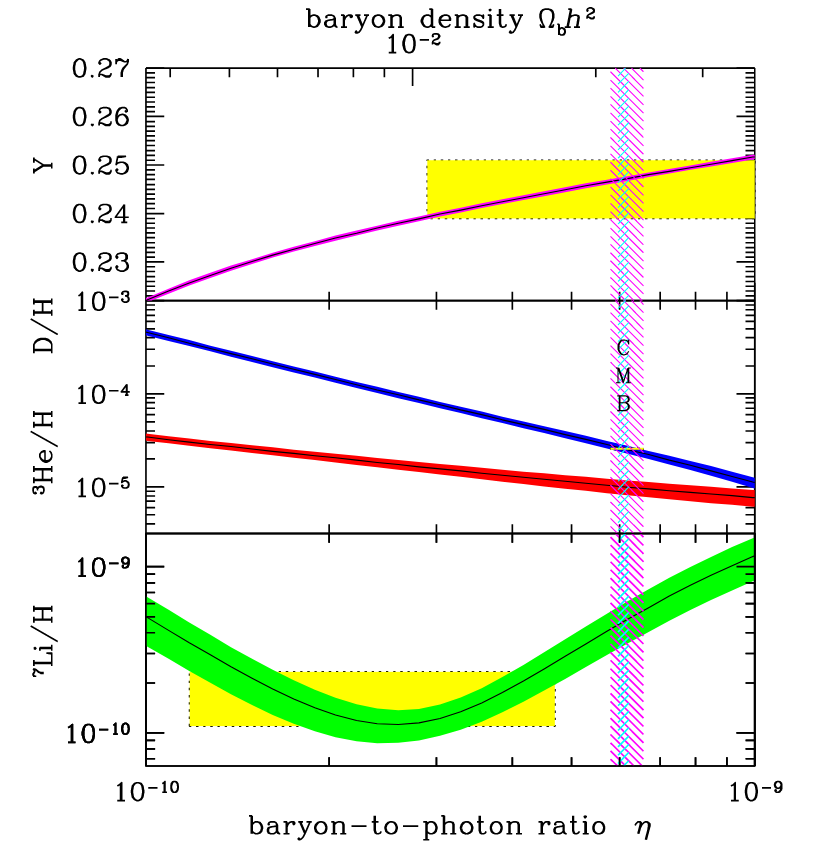
\includegraphics[width=0.6\linewidth]{Figures/BBN.png}
\caption[Variation of Primordial Element Abundances with Baryon-to-Photon Ratio Based on BBN Theory]{Variation of primordial element abundances with baryon-to-photon ratio based on BBN theory. Yellow boxes show the observed range of light element abundances, and the resulting range of baryon-to-photon ratio for three of the light elements. The magenta dashed band shows the estimated baryon-to-photon ratio as determined from the D/H and Y measurements. The blue dashed band shows most recent measurement of the baryon-to-photon ratio from measurements of the CMB with the Planck telescope. Figure reproduced with permission from $\copyright$ \cite{BBN_PDG}.}
\end{figure}

The baryon-to-photon ratio is most sensitive to and best constrained by the primordial abundance of D. Since BBN is the only significant source of D \cite{Deuterium}, which is destroyed in stellar processes, it is important to obtain measurements of the D abundance from regions of space that have not experienced significant stellar nucleosynthesis, which can be identified by their low ``metallicity". Metallicity quantifies the concentration of elements heavier than H and He that would -- with the exception of the small amounts of primordial $^7$Li -- have been produced by stellar nucleosynthesis \cite{Nucleosynthesis}. Studies of low-metallicity gas clouds known as ``damped Ly$\alpha$ systems" \cite{Ly_alpha} can provide a reasonable approximation of the primordial abundance. Fig. 1.5 shows the current constraints on the D/H, $^7$Li/H, and Y as yellow boxes, along with the estimated baryon-to-photon ratio obtained from the D/H and Y abundances, which yields a current best estimate of \cite{BBN_PDG} $0.021 \leq \Omega_b h^2 \leq 0.024$ at a 95\% confidence level. Using h=0.6726$\pm$0.0098 measured by the Planck collaboration \cite{Planck}, we obtain an estimated baryon fraction of $0.046 \leq \Omega_b \leq 0.053$, in agreement with the result from more recent measurements of the CMB. 

The notable inconsistency of $\eta$ obtained from the $^7$Li/H abundance could simply be due to systematic errors in estimating the primordial abundance, or it may present a hint of new physics \cite{BBN_PDG} that is not yet explained by standard BBN theory. 


\subsection{Estimation of $\Omega_M$ from Galaxy Clusters}

In addition to providing strong evidence for dark matter through their collisions (see Section 1.1.2), galaxy clusters can be used to infer the total mass density $\Omega_M$ of the universe from the baryon density $\Omega_b$, under the ``fair sampling assumption". The fair sampling assumption states that because galaxy clusters gather material from a large region of space, their composition provides a fair sample of the universe \cite{DM_Universe}.

While stellar matter composes a fraction of the baryonic matter in galaxy clusters, the majority exists as hot ($\sim$10$^8$K), X-ray emitting ionized gas in the ``intracluster medium" (ICM) \cite{Allen_GasFrac, Vikhlinin_GasFrac}. Under the fair sampling assumption, the total mass density $\Omega_M$ of the universe is obtained from the baryon density $\Omega_b$ and the measured fraction $f_\text{gas}+f_\text{stars}$ of luminous baryonic matter in galaxy clusters according to:

\begin{equation}
\Omega_M = \frac{\Omega_b}{f_\text{gas}+f_\text{stars}}
\end{equation}

In the early 1990's, studies of astronomical data from galaxy clusters \cite{Makino_GasMass} found that for a flat ($\Omega=1$) universe, the baryon fraction $\Omega_b$ inferred from the measured gas mass fraction in the Shapley Supercluster could only agree with earlier results from BBN (see Section 1.2.2) if one assumed that $\Omega_M$ includes a significant non-baryonic dark matter component. 

In a more recent study, \cite{Chandra_Gas_Mass}, data was compiled for 35 luminous clusters collected from NASA's Chandra X-ray observatory. The masses $M_\text{gas}(r)$ and M$_\text{tot}(r)$ of both the ICM gas and the entire cluster were inferred out to a radius $r_{500}$ (the radius at which the cluster density is 500 times the mass density of the surrounding universe at the given redshift) for each galaxy cluster from the density and temperature of the X-ray emitting ionized plasma, under the assumption of hydrostatic equilibrium. The resulting gas fractions $f_{gas}=\frac{M_\text{gas}}{M_\text{tot}}$ shown in Fig. 1.6 were averaged over all galaxies considered.

\begin{figure}[H]
\centering
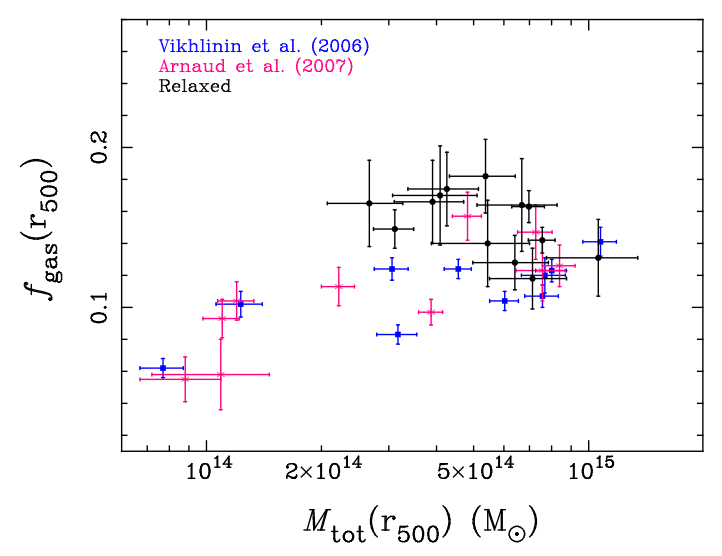
\includegraphics[width=0.7\linewidth]{Figures/Chandra_GasFracs.png}
\caption[Gas Densities of Galaxy Clusters Measured by the Chandra Telescope]{Black: gas densities for the galaxy clusters measured by the Chandra telescope, as a function of cluster mass. Magenta and blue: comparison with previous studies. Figure reproduced with permission from \cite{Chandra_Gas_Mass}. Copyright (2013) by Oxford University Press, on behalf of the Royal Astronomical Society.}
\end{figure}

Combining the average gas mass fraction of $f_\text{gas}=0.163\pm0.032$ with another measurement of stellar baryon fractions out to r$_{500}$ yields $f_\text{gas}+f_\text{stars}=0.182\pm0.032$. Under the fair sampling assumption, this result from galaxy clusters suggests that only 18\% of matter in the universe is accounted for by normal light-emitting baryonic matter.

\subsection{CMB Anisotropies}

First discovered in 1964 \cite{CMB_Discovery}, the cosmic microwave background (CMB) is a faint, approximately isotropic background electromagnetic radiation filling the observable universe, with a mean temperature of 2.73 K \cite{COBE}. Astronomical evidence indicates that the CMB was created following a point in the history of the universe known as the ``recombination epoch". Prior to recombination, the temperature of the early universe was too high for protons and electrons to form neutral atoms. In this ionized plasma, there was a high rate of interactions between photons and free electrons via Thomson and Coulomb scattering \cite{CMB_2015}:

\begin{equation}
\nonumber
e^-+\gamma \leftrightarrow e^-+\gamma
\end{equation}

As a result of these interactions, the universe was at that time opaque to photons. During recombination, the temperature of the universe had cooled to the point that it became energetically favourable for protons and electrons to form neutral atoms. Following recombination, the relatively low interaction probability of photons with neutral atoms made the universe effectively transparent to photons. The escaped photons which comprise the CMB represent the oldest light in the universe, and offer a rich source of information for astronomers studying the conditions of the early universe.

In 1992, the Cosmic Background Explorer (COBE) satellite produced the first evidence of faint anisotropies in the CMB \cite{COBE}, on the order of 1 in 10$^5$. Over its nine-year mission from 2001 to 2009, the Wilkinson Microwave Anisotropy Probe (WMAP) spacecraft \cite{WMAP} measured the CMB radiation with unprecedented precision. The data from WMAP made it possible to produce a detailed map of these anisotropies, and has only recently been overcome in precision following the four-year operation of the Planck telescope \cite{Planck} from 2009 to 2013. These anisotropies reflect the gravitational potential fluctuations in the early universe from which the large-scale structure of the universe is thought to originate. They are typically represented as fractional variations $\Delta T$ from the mean temperature T of the CMB radiation as a function of their direction ($\theta$, $\phi$) in the sky \cite{Hu_CMB_Anisotropies}:

\begin{equation}
\Theta(\theta, \phi) = \frac{\Delta T}{T}
\end{equation}

To study how the size of the temperature fluctuations varies with their angular scale, the fluctuations are commonly transformed into their spherical multipole moments:

\begin{equation}
\Theta_{\ell m} = \int \Theta(\theta, \phi)Y^*_{\ell m}(\theta, \phi)d\Omega
\end{equation} 

where for reasonably small curvature, $\theta=\frac{2\pi}{\ell}$, meaning that $\ell\sim10^2$ represents degree-scale fluctuations \cite{Hu_CMB_Anisotropies}. The resulting power spectrum

\begin{equation}
\langle\Theta*_{\ell m}\Theta_{\ell' m'}\rangle = \delta_{\ell\ell'}\delta_{mm'}C_\ell 
\end{equation}

gives a measure of how the amplitude of the fluctuations varies as a function of their angular scale. 

The ionized plasma that existed prior to recombination can be studied as a ``photon-baryon fluid" \cite{Hu_CMB_Anisotropies}. Small density fluctuations in the fluid produce gravitational wells that attract and compress nearby matter. However, pressure forces due to the Coulomb interactions resist the gravitational compression, acting as an effective spring force to produce oscillatory compression and rarefaction of the fluid. At the time of recombination, photons decoupled from matter, the pressure forces disappeared, and fluctuations in the temperature of the escaped photons forming the CMB reflect the density variations in the photon-baryon plasma at the time of recombination, with higher-temperature photons originating from denser regions of the plasma. The angular temperature fluctuation modes $\ell$ in the CMB correspond approximately to the Fourier wavenumber $k\sim\frac{\ell}{\eta_0}$ of oscillatory modes \cite{CMB_2015}, where $\eta_0$ is the coordinate distance to the last scattering surface. It can be shown \cite{CMB_2015} that for small sections of the sky where curvature can be neglected, the power spectrum $\mathcal{P}_\Theta$ of the oscillatory wavenumber $k\sim\frac{\ell}{\eta_0}$ may be expressed in terms of the angular power spectrum as:

\begin{equation}
\mathcal{P}_\Theta(k/\eta_0) \approx \frac{\ell(\ell+1)}{2\pi}C_\ell
\end{equation}

When this power spectrum is plotted as a function of multipole moment, as shown in Fig. 1.7 with the most recent results from the Planck collaboration, the amplitude of the power spectrum exhibits clear peaks and troughs as a function of angular scale. It is found that the particular shape of the angular scale dependence is well described \cite{Planck} by a flat ``$\Lambda$CDM" Big Bang cosmology \cite{PDG_CosmoParams} containing cold (i.e. non-relativistic) dark matter (CDM), and a cosmological constant $\Lambda$ associated with dark energy. Further, the absolute and relative sizes of the peaks contain information about the composition of the early universe, including the total baryon fraction, and the dark matter component prior to and at the time of recombination. The discussion here of these ``acoustic peaks", and their dependence on the baryon fraction and dark matter component remains largely qualitative, and follows overviews found in \cite{Hu_CMB_Anisotropies, Hu_Website, CMB_2015}. 

\begin{figure}[H]
\centering
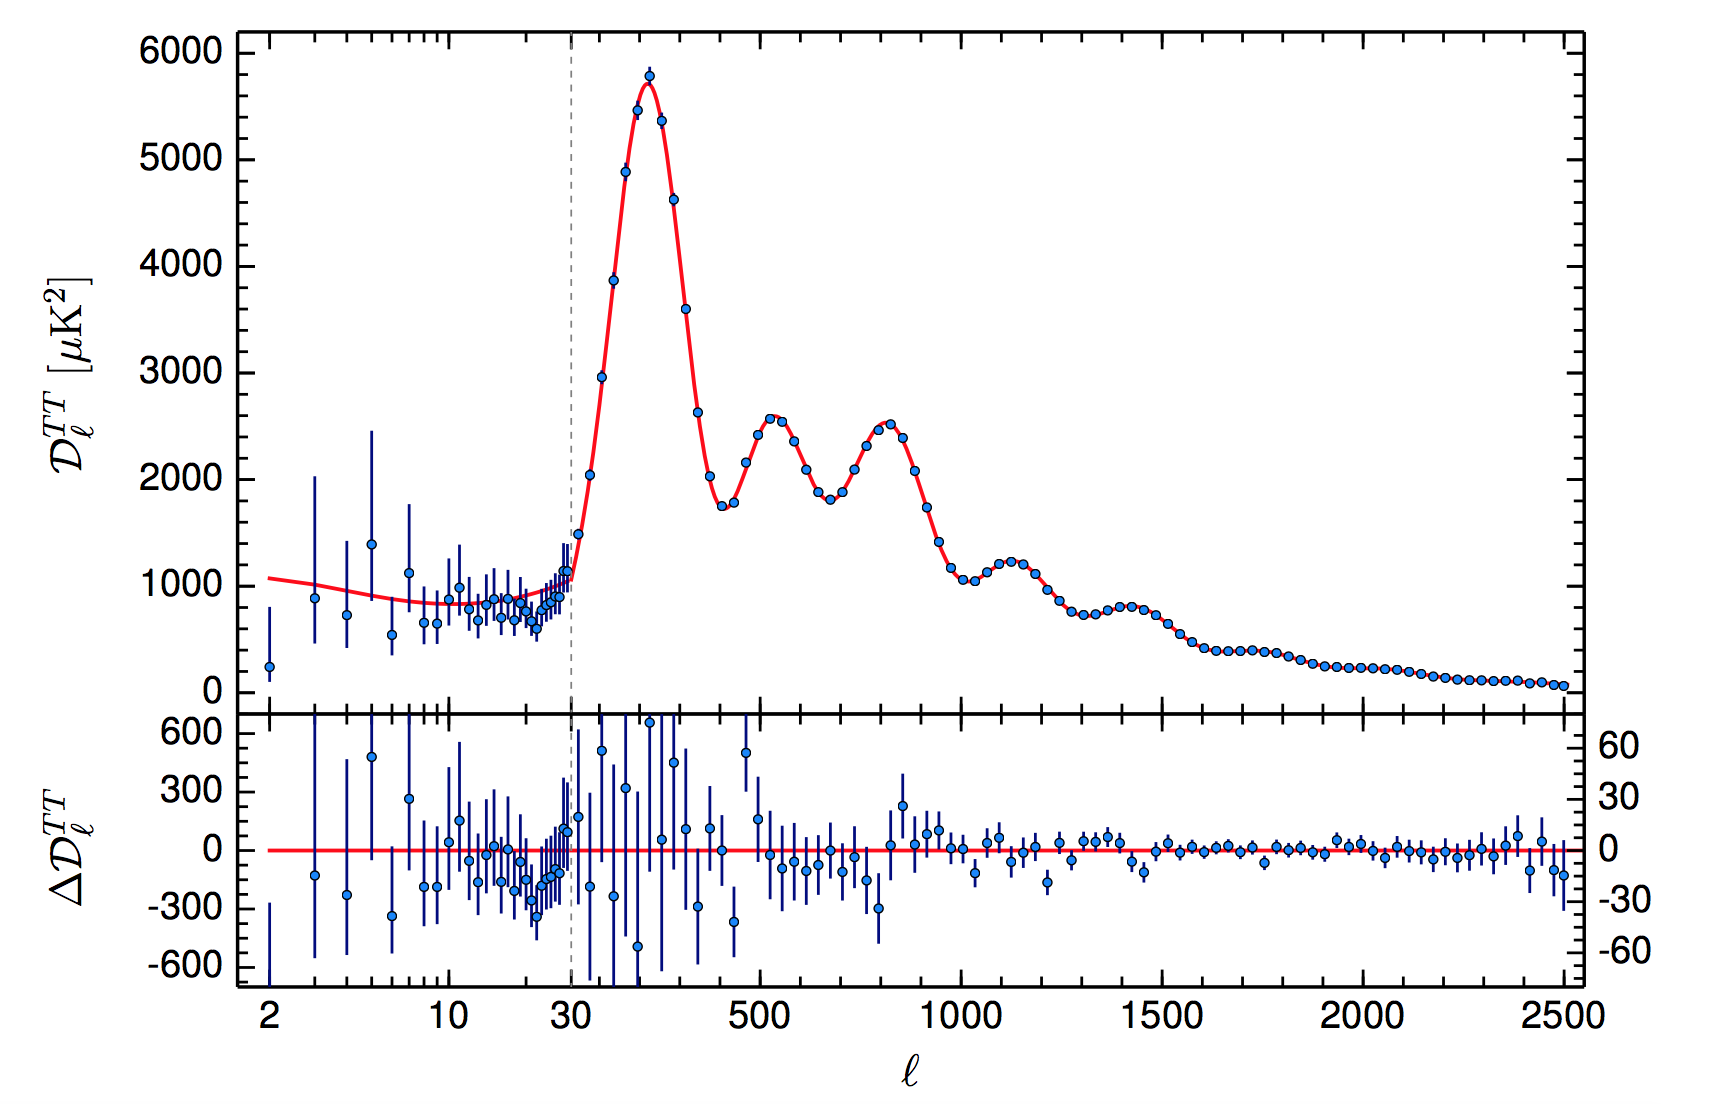
\includegraphics[width=0.8\linewidth]{Figures/Planck_CMB_Anisotropies.png}
\caption[CMB Anisotropies Measured by the Planck Collaboration]{CMB anisotropies measured by the Planck collaboration. The red line shows the prediction of the best-fitting $\Lambda$CDM model for a flat universe ($\Omega=1$). Credit: \cite{Planck}, reproduced with permission $\copyright$ ESO}
\end{figure}

The peaks in the CMB correspond to Fourier oscillation modes of the photon-baryon plasma which reached the extreme maximum of their oscillation at the time of recombination. Assuming that gravitational compression sets up the first stage of oscillation, the first peak corresponds to the ``fundamental" mode $k_f$ that had just reached full compression at recombination, and the second peak corresponds to the mode $2k_f$ that had undergone a full cycle of compression and rarefaction. In a perfect oscillating fluid with instantaneous decoupling at the time of recombination, the power spectrum could be expected to follow a squared sinusoid. 

The first effect that modifies the shape of the CMB peaks is known as ``diffusion". Diffusion arises from the fact that recombination was not instantaneous. Instead, during the short recombination period while particles were combining to form neutral atoms, CMB photons executed a random walk as they interacted with the remaining ionized particles. This random walk `washes out' peaks with wavelengths comparable to or shorter than the distances travelled by photons during their random walk, which introduces the observed exponential damping in the power spectrum at high multipoles. 

The second effect, known as ``baryon loading", is related to the baryon content of the universe at recombination. When the attractive force between massive baryons in the fluid is accounted for, the extremes of compression and rarefaction become asymmetric, because there is now more force pulling the fluid into gravitational wells than there is pushing them out. The effect is that peaks in the CMB spectrum corresponding to compressional extremes of oscillation -- the first, third, fifth, and so on -- become amplified compared with their adjacent peaks. The degree to which odd peaks are enhanced relative to even peaks thus provides information about the baryon density at recombination. 

The third effect, known as ``radiation driving" makes the CMB spectrum sensitive to the dark matter content of the matter-dominated universe leading up to recombination. Prior to recombination, the universe transitioned from the ``radiation-dominated era", during which its behaviour was dominated by radiation, to the ongoing ``matter dominated era" wherein dark matter dominates the behaviour of the universe. During radiation domination, potential wells are formed primarily by photon density fluctuations, which vary with the fluid pressure. As the photon-baryon fluid compresses into these potential wells, the photon density initially increases, deepening the well, then stabilizes as pressure pushes back against the compression. In addition to the shallowing of the well as pressure pushes back against gravity and reduces the photon density, the expansion of the universe further reduces the potential depth, such that the pressure force has very little gravitational potential to overcome during rarefaction. This radiation driving effect enhances the peak amplitudes, but is diminished during the matter-dominated era when the potential wells are formed primarily by pressure-less dark matter. 

The dark matter density $\Omega_\text{DM}$ during the matter-dominated era has two measurable effects on the CMB due to radiation driving. First, the overall degree to which radiation driving is dampened depends on how much dark matter was present over time, where a higher dark matter density induces more damping, and hence leads to smaller peak amplitudes overall. Second, since higher-frequency (i.e. higher-multipole) peaks will have undergone more oscillations during radiation domination, they will exhibit greater enhancement due to radiation driving, such that the exact degree of higher-multipole peak amplitude enhancement is also sensitive to the dark matter density. 

The flat $\Lambda CDM$ model used to fit the CMB power spectrum measured by the Planck collaboration in Fig. 1.7 incorporates the effects discussed above, along with others, to parametrize the shape of the peaks in terms of important cosmological constants. The best fit to the $\ell\geq30$ data in Fig. 1.7 gives a baryon density of  $\Omega_b=0.0491\pm0.0015$, and a cold dark matter density of $\Omega_c=0.2650\pm0.0091$. For a flat universe, these results imply that 26.5\% of the universe is composed of dark matter, and only 4.9\% of normal baryonic matter.  

 
\section{Composition Hypotheses}

The previous section presented three lines of evidence, which together strongly suggest that the majority of matter in the universe is dark, and that only a small portion of this dark matter could be accounted for by normal baryonic matter. There is nothing in the current Standard Models of cosmology or particle physics \cite{DM_Candidates} that can account for such a significant fraction of the mass budget of the universe.  

Theories known as ``modified gravity" have been developed that modify general relativity \cite{MOND} in order to avoid the need for dark matter entirely. Others modify the standard inflationary cosmology to allow for the development of ``primordial black holes" \cite{PBH} prior to BBN, which would not be accounted for in the estimates of $\Omega_b$ based on BBN theory and measurements of the CMB. However, these modified theories have so far suffered significant theoretical and/or observational hurdles, such as difficulties with using modified gravity to explain the evidence for dark matter on cosmological scales, and fine-tuning assumptions associated with the development of primordial black holes in the early universe \cite{PBH}. The current most widely accepted dark matter candidates take the form of particles associated with theories beyond the Standard Model (SM) of particle physics. 

In order to represent a significant contribution to the dark matter content of the universe, candidate particles must satisfy several basic criteria \cite{DM_PDG}. First, they must be stable on cosmological time scales -- otherwise they would have decayed away by now. Second, analysis of structure formation in the universe suggests that particle dark matter should be ``cold", meaning that it was non-relativistic when galaxies began to form. Third, to constitute a significant fraction of the observed dark matter density $\Omega_\text{CDM}$, they must have the correct ``relic density" at the time that their interaction rate became negligible with SM particles. Lastly, dark matter must be effectively ``collisionless" \cite{Axions_2009}, meaning that the only significant long-range interactions are gravitational.
%i.e. density at the time that the falling temperature and density due to the expansion of the universe caused its interaction rate to became negligible, hence decoupling it from other matter and fixing its abundance

Of the hypothesized particles satisfying the above criteria, weakly interacting massive particles (WIMPs) and axions have for a number of years been considered the most theoretically and experimentally viable particle dark matter candidates, and have been the subject of many dedicated experimental searches. 

The axion was originally proposed as a part of the Peccei-Quinn \cite{Axions_PQ} solution to the strong CP problem in quantum chromodynamics (QCD). The strong CP problem arises from the fact that although the strong interaction contains a CP-violating term in its Lagrangian, CP violation has not been observed in QCD interactions. Axions would have been produced ``non-thermally" \cite{DM_PDG}, meaning that they were not in thermal equilibrium with SM particles in the early universe. This allows them to have masses as low as $\mu$eV, much lower \cite{DM_PDG, Axions_2009} than would be allowed for ``thermally-produced" dark matter, as will be discussed further in the next section. The axion, and axion-like particles (ALPs) are predicted to decay into pairs of SM particles \cite{Axion_Decay}, thus presenting a possibility for experimental detection. 

The axion would reside in one of potentially many hidden ``dark sectors" \cite{DarkSector} that interact through their own particles, forces, and structure, with only very weak couplings to SM particles. More recent theoretically-motivated candidates from the dark sector include the ``dark photon", whose couplings with electrically charged particles through kinetic mixing with the SM photon could provide the possibility for experimental detection \cite{DarkSector}. 

%WIMPs represent a popular class of dark matter candidates that originally were largely associated with supersymmetric extensions of the Standard Model, but have more recently been predicted in association with non-supersymmetric theories as well. As they 

The remainder of this chapter will be devoted to WIMPs -- the primary search candidate of the SuperCDMS experiment -- with particular emphasis on low-mass WIMP candidates to which SuperCDMS is particularly sensitive.  

\subsection{WIMPs}

WIMPs represent a general class of massive, non-baryonic fundamental particles that interact gravitationally with normal matter, and whose interactions with SM particles are at or below the weak interaction strength, but non-negligible \cite{WIMP_Candidates}. This broad definition could in fact encompass any of the axions and dark photon candidates discussed above, but in practice, WIMPs are often considered to have masses in the approximate range of $\sim$10 GeV - TeV predicted by minimal supersymmetric models \cite{DM_Candidates}, with low-mass WIMPs (which may be unrelated to supersymmetry) occupying the approximate mass range of several MeV to 10 GeV. 

\subsubsection{Thermal Freeze-Out and the WIMP Miracle}

As the abundance of many popular WIMP candidates is predicted to arise from ``thermal freeze-out" in the early universe \cite{WIMP_Candidates}, the mechanism for thermal freeze-out is briefly discussed here. According to the thermal freeze-out hypothesis, WIMPs were in thermal equilibrium with SM particles in the high temperature and matter density of the early universe. As the universe expanded and cooled, the interaction rate declined. Once the WIMP-SM interaction rate dropped below the expansion rate of the universe, the WIMPs rapidly ``froze out" of thermal equilibrium with the SM particles, effectively fixing the co-moving WIMP density to its present-day value \cite{WIMP_Candidates}. The present-day WIMP dark matter density $\Omega_\chi h^2$ is then approximately given by \cite{Beyond_Thermal_WIMPs}:

\begin{equation}
\frac{\Omega_\chi h^2}{0.12}\approx \frac{1}{\Big\langle \frac{\sigma_\text{ann}}{10^{-36}\text{cm}^2}\frac{v/c}{0.1}\Big\rangle}
\end{equation}

For expected WIMP velocities at freeze-out ($v/c\approx0.1$), the interaction cross section of 10$^{-36}$cm$^2$ corresponding to the present-day dark matter density ($\Omega_\text{DM}h^2\approx0.12$) is at a scale typical for interactions mediated by the weak force. This apparent coincidence was dubbed the ``WIMP miracle", and spurred significant interest in dark matter candidates with weak-scale cross sections and typical weak force masses in the range of $\sim$10 GeV/c$^2$ to several TeV.
%, with masses in the range of ~10 GeV/c$^2$ to several TeV. 
It has however been argued \cite{WIMPless_Miracle} that the WIMP mass need not necessarily be constrained to the above ``weak force" range in order to produce weak scale WIMP-SM interaction cross sections. 

\subsubsection{Supersymmetric WIMPs}

Many supersymmetric models predict a stable particle with weak-scale interactions and a mass in the range of $\sim$10 GeV/c$^2$ to several TeV/c$^2$ as part of a solution to the ``hierarchy problem" \cite{DM_Candidates} in particle physics. The hierarchy problem is the question of why the physical Higgs boson mass is so much smaller than the Planck mass scale. 

The apparent naturalness of supersymmetric WIMP candidates arising from a solution to an independent problem, combined with the popularity of supersymmetry as an extension to the SM, has for many years made it the most important candidate for many experimental dark matter searches. However, dedicated experimental searches have so far failed to find evidence for the most constrained supersymmetric WIMP models \cite{DM_PDG}. These null results, combined with the absence of evidence for supersymmetry at the LHC \cite{LHC_SUSY, CMS_SUSY}, have motivated increasing interest in theories predicting WIMPs outside of the traditional mass range of $\sim$10 GeV/c$^2$ to several TeV. The following section discusses in particular theories predicting relatively low-mass dark matter, in the sub-GeV/c$^2$ to $\sim$10 GeV/c$^2$ range.

\subsubsection{Low-mass WIMP Hypotheses}

Of the numerous theories that have emerged in recent years with low-mass WIMP predictions, some arise from non-traditional extensions of supersymmetry, such as models with an extended Higgs sector \cite{DM_PDG}, or others predicting axinos and gravitinos -- fermionic partners of the axion and graviton, respectively -- as dark matter constituents \cite{Beyond_Thermal_WIMPs}. However, many of the more recent low-mass WIMP theories are entirely unrelated to supersymmetry, and may invoke either thermal or non-thermal production mechanisms. 

Asymmetric dark matter (ADM) is an example of a non-supersymmetric model with low-mass WIMP predictions. The theory allows for various possible mechanisms for interaction with SM particles, and WIMP masses in the range of $\sim$5-15 GeV/c$^2$ \cite{Asymmetric_DM}. In this model, WIMPs are not their own antiparticle, and the observed abundance of dark matter is assumed to arise not from the details of its thermal decoupling, but rather from a mechanism analogous to that which produced the observed baryon-antibaryon asymmetry in the universe. It is argued \cite{Asymmetric_DM} that this common origin of baryon and dark matter abundances could account for the fact that the observed densities are of similar magnitudes ($\Omega_\text{DM}\approx5\Omega_b$), a result which may otherwise appear coincidental.

Other potential candidates could arise from the hidden dark sector introduced earlier. The massive dark photon, with predicted masses ranging from MeV/$c^2$ to GeV/$c^2$ depending on the details of its origin and ``portal interactions" with SM particles \cite{DarkSector}, would couple through the ``vector portal", one of four possible dominant interaction portals between SM and dark sector particles. Many of the early exclusion limits for dark sector candidates have come from reanalyses of existing WIMP search data \cite{DarkPhoton_WIMP}. However, future experiments, including a planned search for dark photon absorption events in SuperCDMS single-charge sensitive detectors \cite{SuperCDMS_DarkPhoton}, could offer targeted sensitivity to predicted portal interactions. 


\chapter{WIMP Detection Techniques}

The last chapter presented several lines of observational evidence indicating that $\sim$85\% of the matter in the universe is cold (i.e. non-relativistic) non-luminous ``dark matter" that interacts via the gravitational force, but otherwise very weakly -- if at all -- with either itself or normal matter. While observational data has provided precise determinations of the dark matter makeup of the universe, it fails to answer some important questions, such as:

\begin{itemize}
\item Assuming that dark matter is composed of elementary particles, what are the properties of these particles (mass, spin, etc.)?
\item By what mechanisms other than gravity does dark matter interact with itself and/or other matter?
%\item How was dark matter produced in the early universe such that it exists with its observed present-day density?
\end{itemize}

This chapter will discuss the techniques that are employed to detect particle dark matter (DM) in the hopes of understanding its particle properties and non-gravitational interactions. These dark matter detection techniques are divided into three classes -- accelerator searches, indirect detection, and direct detection -- which are summarized in Table 2.1, and discussed in more detail in the next three sections, focusing on WIMP detection. Particular emphasis is given to direct detection, which is the method employed by the SuperCDMS experiment.

\begin{table}[H]
\centering
\caption[Dark Matter Search Modes]{Summary of the three primary dark matter search modes}
\label{my-label}
\begin{footnotesize}
\renewcommand{\arraystretch}{1.5}
\begin{tabular}{|p{40mm}|L{55mm}|L{25mm}|}
\hline
\textbf{Search Mode} & \textbf{Summary} & \textbf{Examples}  \\ \hline
Direct Detection & Directly measure elastic WIMP-nucleon scattering in a low-background environment  & SuperCDMS, EDELWEISS, DEAP 3600               \\ \hline
Accelerator Searches       & Search for missing total or transverse momentum in high-energy collisions, indicating the production of new stable, neutral particles.     & ATLAS, CMS, Belle II                \\ \hline
Indirect Detection      & Use observational data to detect products of WIMP annihilations or decays in regions of the observable universe that are expected to have a high dark matter density    & PAMELA satellite, HESS telescope               \\ \hline
\end{tabular}
\end{footnotesize}
\end{table}

\section{Direct Detection}

Most of the WIMP search experiments employ some form of direct detection. For this search mode, detectors are operated in a low-background environment, typically underground, and experiments look for an above-background excess of nuclear recoil events that could be attributed to WIMP-nucleon collisions in the detectors. 

\subsection{Predictions for WIMP-nucleon Interactions on Earth}

It is expected that WIMPs should be present in our Milky Way galaxy with the appropriate density profile to produce the rotation curves measured in other galaxies (see Section 1.1.1). Given the expected speed of WIMPs relative to terrestrial detectors -- typically taken to be $\sim$220 km/s on average \cite{Direct_Searches_Saab} -- it is expected that the dominant interaction mechanism will be elastic scattering in the detector \cite{Direct_Searches_Saab}. For WIMP masses comparable to or larger than the proton mass ($\gtrsim100$ MeV/$c^2$), it is kinematically favourable for WIMPs to interact via nuclear recoils, rather than electron recoils, in the detector material. 

The interaction rate of WIMPs with terrestrial detectors depends on both the interaction cross section -- which is material dependent -- and the local WIMP flux. The WIMP flux is set by the local dark matter density (most recently calculated at 0.39 GeV cm$^{-3}$ \cite{Local_DM}), the mean WIMP velocity, the escape velocity $v_{esc}\approx544$ km/s \cite{Escape_Velocity} of the Milky Way galaxy, and the WIMP mass. Therefore, the two unknowns in predicting the rate of WIMP-nucleon interactions with a given detector material are the WIMP mass m$_\chi$ and WIMP-nucleon scattering cross section $\sigma_0$. For this reason, WIMP exclusion limits from direct detection searches are typically shown as upper bounds on the WIMP-nucleon interaction cross section as a function of WIMP mass, as shown in Fig. 2.1 with a compilation of recent exclusion limits from direct detection experiments on ``spin-independent" WIMP-nucleon couplings. Spin-independent couplings are characterized by scalar and vector WIMP-nucleon currents \cite{DM_PDG}. Exclusion limits also exist for ``spin-dependent" couplings, which involve axial vector currents \cite{DM_PDG} and assume that WIMPs have a non-zero spin, but accelerator searches are typically more sensitive to these couplings than direct detection searches (see Section 2.2). 

\begin{figure}[H]
\centering
\makebox[\textwidth][c]{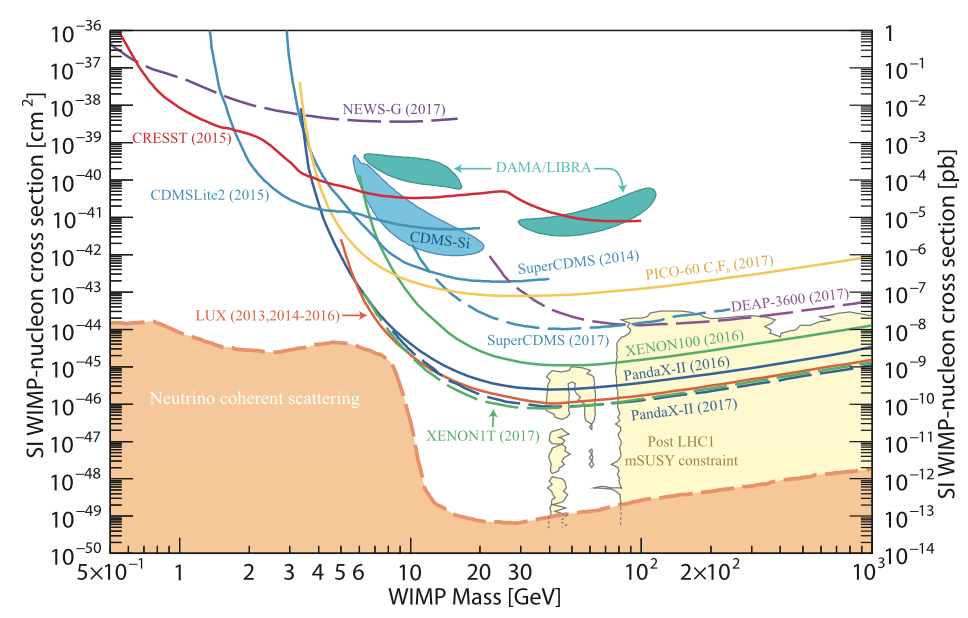
\includegraphics[width=1.3\linewidth]{Figures/Direct_Constraints.png}}
\caption[WIMP-nucleon cross section exclusion limits from direct detection searches for spin-independent coupling]{WIMP-nucleon cross section exclusion limits from direct detection searches for spin-independent coupling. Figure reproduced with permission from $\copyright$ \cite{DM_PDG}.}
\end{figure}

For spin-independent couplings, the WIMP-nucleon scattering cross section $\sigma_0$ is expected to vary with the atomic number $A$ of the target nucleus according to \cite{Direct_Searches_Saab}: $\sigma_0\propto A^2\sigma_{\chi-p}$, where $\sigma_{\chi-p}$ is the WIMP-proton interaction cross section. Therefore, it is often desirable to select a target material with a high atomic number for direct detection searches, though other details such as the nuclear form factor $F(Q)$ \cite{Direct_Searches_Saab} and background rejection possibilities can also affect the choice of target material. It is also important to consider the range of recoil energies that can be accurately measured by the detector. For non-relativistic scatters, the nuclear recoil energy is related to the WIMP mass and scattering angle $\theta_r$ according to \cite{Directional_DM}:

\begin{equation}
E_r = 2v^2\frac{\mu^2}{m_A}\cos^2\theta_r
\end{equation}

where $m_A$ is the mass of the target nucleus, $\mu=m_\chi m_A/(m_\chi+m_A)$ is the WIMP-nucleus reduced mass, and $v$ is the WIMP speed in the laboratory rest frame. Depending on the WIMP and target masses, this can result in nuclear recoil energies in the range of 0 to $\sim$100 keV. 

The lower bound on the WIMP masses to which direct detection searches are sensitive is in general dictated by the signal to noise ratio of the detector(s). As the WIMP mass decreases, the average nuclear recoil energy $E_r$ imparted to the nucleus in a WIMP-nucleon collision will also decrease based on Eq. 2.1, and at some point the measured recoil energy will become indistinguishable from detector noise. Near this ``noise wall", it becomes increasingly difficult to place strong constraints on the interaction cross section, resulting in the characteristic sharp rise in cross section limits seen at low WIMP masses in Fig. 2.1.


\subsection{Background Discrimination Methods}
For typical values of $\sigma_0$ and m$_\chi$, predicted signal event rates are on the order of 1 event year$^{-1}$ kg$^{-1}$ \cite{Direct_Searches_Saab}, much lower than the typical radioactive background on Earth's surface \cite{DM_PDG}. This background can be reduced by operating the detectors deep underground to minimize the flux of cosmic rays, surrounding the detector with additional radioactive shielding, and selecting radio-pure materials for the detectors and surrounding structure. In addition, most direct-detection experiments employ some form of background discrimination to minimize the number of background events that can be interpreted as WIMP signals. Active detector shielding, such as a cosmic ray veto surrounding the detector, is a common method of identifying measured events as background. Other discrimination techniques aim to identify predicted temporal variations in the flux or directionality of signal events \cite{Direct_Searches_Saab}. 

Annual modulations in the WIMP flux are predicted due to the change in relative velocity between Earth and the galaxy's WIMP halo. The DAMA collaboration \cite{DAMA} has reported a 9.3 $\sigma$ annual modulation in their signal rate with a total of 13 years of data-taking and 350kg of detector material, with the possible WIMP masses and cross sections of the signal enclosed by the turquoise DAMA/LIBRA regions in Fig. 2.1. Since the first announcement of the DAMA/LIBRA annual modulation signal, other WIMP searches have explored the same parameter space, with null results. Yet, a convincing alternative explanation of the annual modulation has yet to be demonstrated. 

Daily modulations in the directionality of WIMP recoil events are predicted due to Earth's rotation as it travels through the WIMP halo \cite{Direct_Searches_Saab}, with an excess of nuclei recoiling in the direction of the ``WIMP wind". Identifying this directionality requires detectors capable of reconstructing the tracks of measured particles, such as the gaseous detectors employed by the DRIFT experiment \cite{DRIFT}. 

The annual and daily modulation effects described above are statistical in nature, and can only be resolved with a reasonably large set of candidate signal events. Another approach is to use expected differences in detector response to WIMP vs. background events to discriminate on an event-by-event basis. This technique is applied in solid state detectors such as SuperCDMS and EDELWEISS, where differing amounts of ionization are expected for nuclear vs. electron recoil events of the same energy. The ionization signal is compared with the total event energy to discriminate nuclear recoils of interest from the electron recoil background.

\section{Accelerator Searches}

At particle colliders such as the LHC, the WIMP detection strategy is to collide hadrons or leptons at a sufficient rate and energy such that WIMPS could be produced at a measurable rate. One can then use the fact that the total momentum of all particles produced by a collision should nominally sum to 0 in the direction transverse to the beam line. Due to the negligible interaction probability of WIMPs with the detector material, WIMP searches with collider data look for events with an excess of missing momentum transverse to the beam line. Such an excess could suggest that one or more neutral and stable (or at least long-lived) particles passed through the detector without depositing energy, thus satisfying two of the four criteria identified in Section 1.3 to represent a viable dark matter candidate. 

%The most common and model-independent search channel \cite{LHC_DM} is a system of observable particles such as a photon or a ``jet" --  i.e. a collimated bundle of particles -- recoiling against a pair of WIMPs. 
Since neutrinos also have a very low probability of interacting in the detector, Standard Model (SM) processes that produce neutrinos in their final states can also result in missing transverse momentum. Such processes can represent a significant background \cite{LHC_DM} in accelerator WIMP searches. 

Constraints on WIMP properties obtained from accelerator searches can, using various assumptions \cite{LHC_DM}, be converted to upper limits on the WIMP-nucleon interaction cross section as a function of WIMP mass for ease of comparison with direct detection search constraints. Such a comparison is shown in Fig. 2.2, with accelerator constraints determined from LHC data collected by the ATLAS detector. 

\begin{figure}[H]
\centering
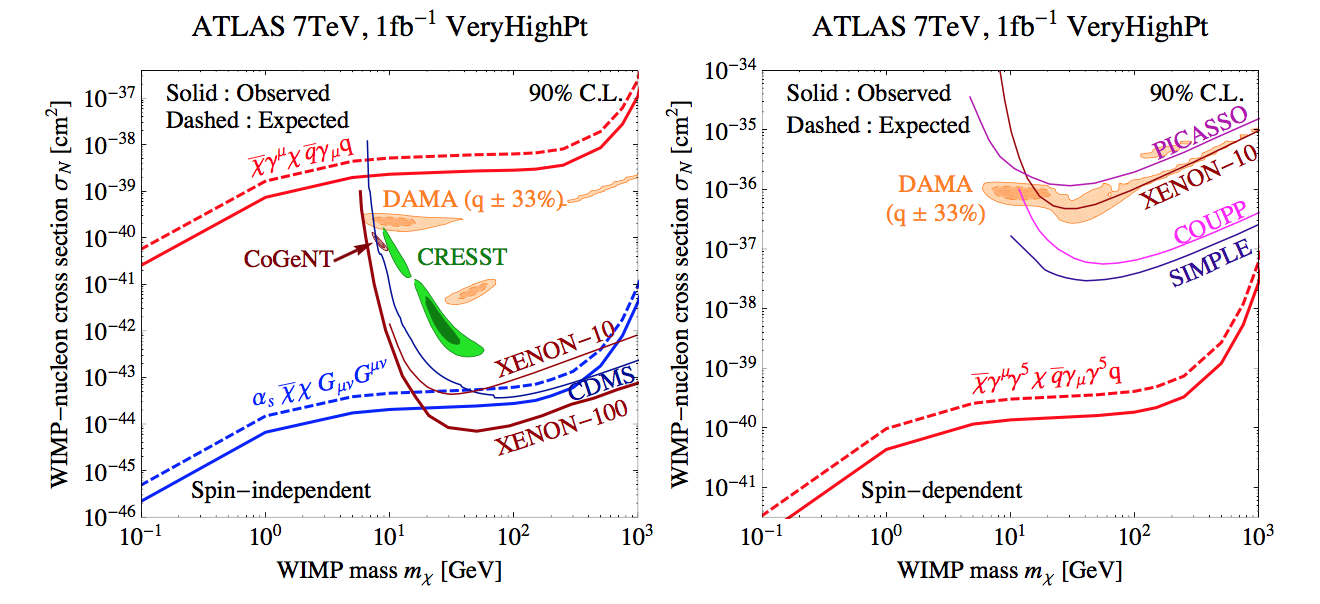
\includegraphics[width=\linewidth]{Figures/LHC_Constraints.png}
\caption[Comparison between upper bounds on the WIMP-nucleon interaction cross section obtained from accelerator vs. direct detection searches]{Comparison between upper bounds on the WIMP-nucleon interaction cross section obtained from accelerator vs. direct detection searches. Left: Constraints for spin-independent WIMP-nucleon coupling. Right: Constraints for spin-dependent coupling. See Section 2.1.1 for definition of spin-independent and spin-dependent couplings. Reprinted figure with permission from \cite{LHC_DM}. Copyright (2012) by the American Physical Society.}
\end{figure}

Comparing the accelerator constraints (red and blue) in Fig. 2.2 with direct detection constraints, it is clear that accelerator searches can offer complementary limits. This is particularly true for sub-GeV/c$^2$ WIMP masses range where the sensitivity of direct detection searches tends to drop off quite steeply due to their low-energy noise threshold.

%Accelerator searches can be sensitive to both ``spin-dependent" and ``spin-independent" couplings of dark matter with SM particles \cite{LHC_DM}. Spin-dependent couplings . Collider experiments are also 

\section{Indirect Detection}

Indirect WIMP detection uses observational data to search for unique spectral signatures showing an excess of one or more cosmic rays (CRs) (e$^\pm$, $\bar{p}$, $\gamma$, $\nu$) which cannot be explained by any known astrophysical process. Such signatures could be produced by hadronization following the annihilation of two WIMPs, forming a pair of SM particles \cite{Indirect_Searches}. Indirect detection searches typically focus on regions of space, such as galaxy clusters and the centre of the Milky Way galaxy \cite{Indirect_CR}, that are expected to have a relatively high density of dark matter.

Since ordinary astrophysical processes produce a significant background of CRs \cite{Indirect_CR}, accurately modelling these background processes is important for the sensitivity of indirect WIMP searches. Further, it is useful to select decay channels and energy ranges with a relatively low flux of CRs from background processes \cite{Indirect_Searches}. For example, it is common for indirect detection searches to focus on antiparticle CRs rather than the corresponding particle flux due to the relatively low background abundance of antiparticles. 

Indirect searches are particularly suited for studying WIMP masses near or above the TeV range \cite{Indirect_CR, Indirect_Searches}, and thus have the potential to complement both accelerator searches, as well as direct detection searches which focus primarily on the sub-GeV to $\sim$TeV range. 

\chapter{Overview of the SuperCDMS Experiment}

The Super Cryogenic Dark Matter Search (SuperCDMS) is an experiment that aims either to directly detect particle dark matter candidates, or to place constraints on the properties of proposed particles, such as their mass and interaction cross section. The primary search candidate -- and the one which I will discuss primarily in this thesis -- is the hypothetical WIMP particle. 
%To search for WIMPs, the experiment looks for an excess of nuclear recoil events above the neutron-induced background that could be attributed to WIMP-nucleon collisions in the SuperCDMS detectors. 

The first generation of direct detection WIMP search experiments were primarily sensitive to WIMP masses ranging from a few GeV/c$^2$ to a few TeV/c$^2$, based on the expectation that the WIMP could be a stable supersymmetric particle \cite{SupersymmetricDarkMatter}. Not yet having found convincing evidence from direct detection experiments for WIMPs in this mass range, nor evidence for supersymmetry at the LHC \cite{LHC_SUSY, CMS_SUSY}, recent theoretical work \cite{Asymmetric_DM, DarkSector} has predicted WIMPs with masses near or below 10 GeV/c$^2$, some of which are unrelated to supersymmetry. SuperCDMS is designed to be sensitive to these low-mass WIMP candidates that would be below the detection threshold of most other dark matter search experiments.

To attain the low-background environment required to search for rare WIMP-nucleon collisions, the detectors are operated deep underground, thereby minimizing the flux of cosmic rays. Having recently established a world-leading limit on the spin-independent WIMP-nucleon cross section for a WIMP mass as low as $\sim$3 GeV/c$^2$ \cite{CDMSlite_long} following four years of operation 780m underground at the Soudan laboratory in Minnesota, the experiment will continue the low-mass WIMP search $\sim$2km underground in the SNOLAB facility near Sudbury, Ontario. Fig. 3.1 shows the projected sensitivity of the SuperCDMS experiment at SNOLAB.

\begin{figure}[H]
\centering
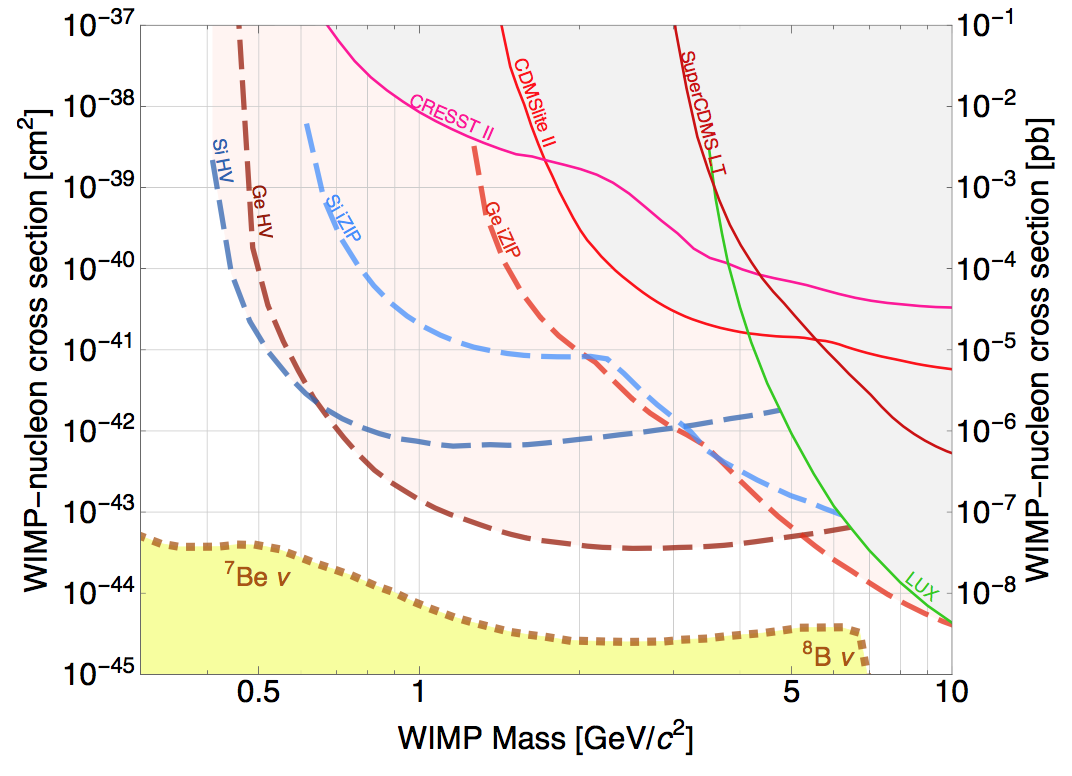
\includegraphics[width=0.6\linewidth]{Figures/ProjectedSensitivity.png}
\caption[Projected Sensitivity at SNOLAB]{Projected sensitivity of the SuperCDMS experiment at SNOLAB. Reprinted figure with permission from \cite{Projected_Sensitivity}. Copyright (2017) by the American Physical Society}
\end{figure}

The experiment uses solid-state silicon and germanium detectors that detect both tiny vibrations in the crystal lattice, called phonons, and ionization (electron-hole) pairs produced when an incident particle scatters elastically off a nucleus in the detector \cite{NewResults}. The electron-hole pairs are measured by aluminum electrodes patterned as shown in Fig. 3.2 on either detector face, which at Soudan were amplified and read out by Field Effect Transistors (FETs). These FETs will be replaced with High Electron Mobility Transistors at SNOLAB due to their reduced readout noise and power dissipation \cite{SNOLAB_Tower}. 

In order to detect the minute phonon signals generated by low-energy particles scattering in the detector, aluminum collection fins on the two detector faces are coupled to tungsten conductors cooled to their superconducting transition temperature, on the order of 50 mK \cite{CDMSII}. At this temperature, a small increase in temperature caused by an incident phonon will result in a drastic change in the conductor's resistance. For this reason, the detector is known as a ``transition-edge sensor" (TES). The change in resistance can be measured by a change in the current flowing through the conductors. The current signal is further amplified by a superconducting quantum interference device (SQUID) circuit. The SQUID outputs a measurable voltage signal pulse in response to a magnetic flux though its superconducting loop induced by the change in current \cite{SQUIDs}. 

The analysis discussed in Chapter 4 uses calibration data collected from germanium SuperCDMS detectors at Soudan, which were an upgrade to the older CDMS II detectors also operating at Soudan \cite{CDMSII_orig}.

\section{Detectors and Experimental Setup}

The SuperCDMS Soudan Ge detectors, having the approximate dimensions of a hockey puck, are stacked into vertical arrays of three detectors known as ``towers", of which five were running at Soudan. The detector stacking is advantageous for the rejection of nuclear recoil events due to neutrons, because neutrons will often scatter in multiple detectors, whereas a WIMP would only be expected to scatter once due to the low interaction cross section \cite{Soudan_FirstResults}.  

The detector towers are located in a low-radioactivity copper cryostat, which is coupled via nested tubes known as the ``C-stem" to a helium dilution refrigerator to maintain a base temperature between 40 and 50 mK. 

The overburden of 780 m of rock, or 2090 meters water equivalent, reduces the flux of cosmic ray muons by a factor of 5$\times$10$^4$ \cite{Soudan_FirstResults}. Additional shielding is provided by successive layers of copper ($\sim$0.5 cm), lead (22.5 cm), and polyethylene (50cm) shielding \cite{Soudan_FirstResults} surrounding the cryostat, as shown in Fig. 4.5 in Chapter 4, to reduce the background of gammas and neutrons from radioactive and cosmogenic sources that would reduce the sensitivity of the experiment. Surrounding this shielding is an active veto to tag cosmic rays, which consists of 5.2 cm thick plastic scintillator panels read out by photomultiplier tubes \cite{DAQ_CDMSII, Soudan_FirstResults}. 

\begin{figure}[H]
\centering
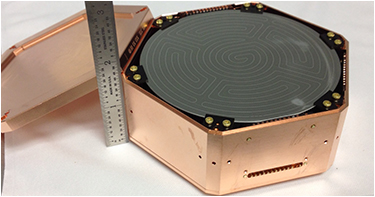
\includegraphics[width=0.6\linewidth]{Figures/PhysicalDetector.jpg}
\caption[SuperCDMS Soudan Detector]{Sample SuperCDMS iZIP detector used at Soudan. Figure from SuperCDMS collaboration standard public plots \cite{SuperCDMS_website}.}
\end{figure}

When a pulse is measured by the phonon and ionization sensors, the first stage of SQUID and FET amplification, respectively, takes place within the cryostat \cite{DAQ_CDMSII}. The signals are then carried to the room-temperature data acquisition electronics, discussed in the next section, via copper-kapton cables. 

\section{Data Acquisition and Triggering}

Fig. 3.3 shows the channel layout of the SuperCDMS Soudan detectors used for the photoneutron analysis in Chapter 4. The phonon sensors on each detector face are divided into four channels, with three inner channels labelled B, C, and D, and an outer channel labelled A. Each phonon channel produces a separate pulse, which is subsequently read out by the data acquisition electronics. The relative pulse shapes and amplitudes in the four phonon channels enable some degree of position sensitivity, which is important for defining fiducial volume cuts. There are two charge channels, divided into an inner disk and an outer ring, each of which produces a separate pulse. 

\begin{figure}[H]
\centering
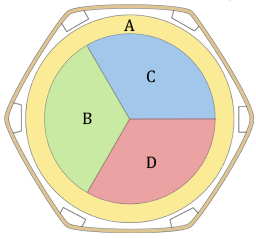
\includegraphics[width=0.5\linewidth]{Figures/ChannelLayout2.png}
\caption[SuperCDMS Detector Channel Layout]{SuperCDMS Detector Channel Layout. Figure from SuperCDMS collaboration public website \cite{SuperCDMS_experiment}.}
\end{figure}

Following a measured recoil event in a detector, the six electrical signals -- four phonon and two ionization -- arriving from the SQUID and FET amplifiers are read into the detector's room temperature front end board (FEB) for further amplification. From the FEB, the signals are directed to the Receiver/Trigger/Filter board, which passes them through a low-pass filter and digitizes them. Trigger information is determined separately for the phonon and ionization signals in the RTF board by summing each signal over all channels and comparing the summed waveforms with adjustable high and low thresholds. The resulting high and low trigger bits are fed into the trigger logic board (TLB), which makes and records the final trigger decision based on the set trigger condition \cite{DAQ_CDMSII}. The trigger condition could be, for example, one of the following:

\begin{itemize}
\item passing the phonon low threshold (P$_\text{low}$)
\item passing both phonon and charge low thresholds, but failing the phonon high threshold (P$_\text{low}$ Q$_\text{low}$, NOT P$_\text{hi}$)
\end{itemize}


\section{Detector Operating Modes}

SuperCDMS detectors can be operated in two distinct modes, known as ``iZIP" (interleaved Z-sensitive Ionization Phonon) and ``CDMSlite" (Cryogenic Dark Matter Search low ionization threshold experiment). Of the two, the CDMSlite operating mode is a more recent development, and will be the primary mode discussed in the remainder of this thesis.

\subsection{iZIP Mode}

In iZIP mode, the detector is operated with a 4V bias across the ionization collectors on either detector face, and both faces are used for both charge and phonon signal readout. The 4V bias voltage is optimized to be as low as possible while enabling full charge collection. 

\begin{figure}[H]
\centering
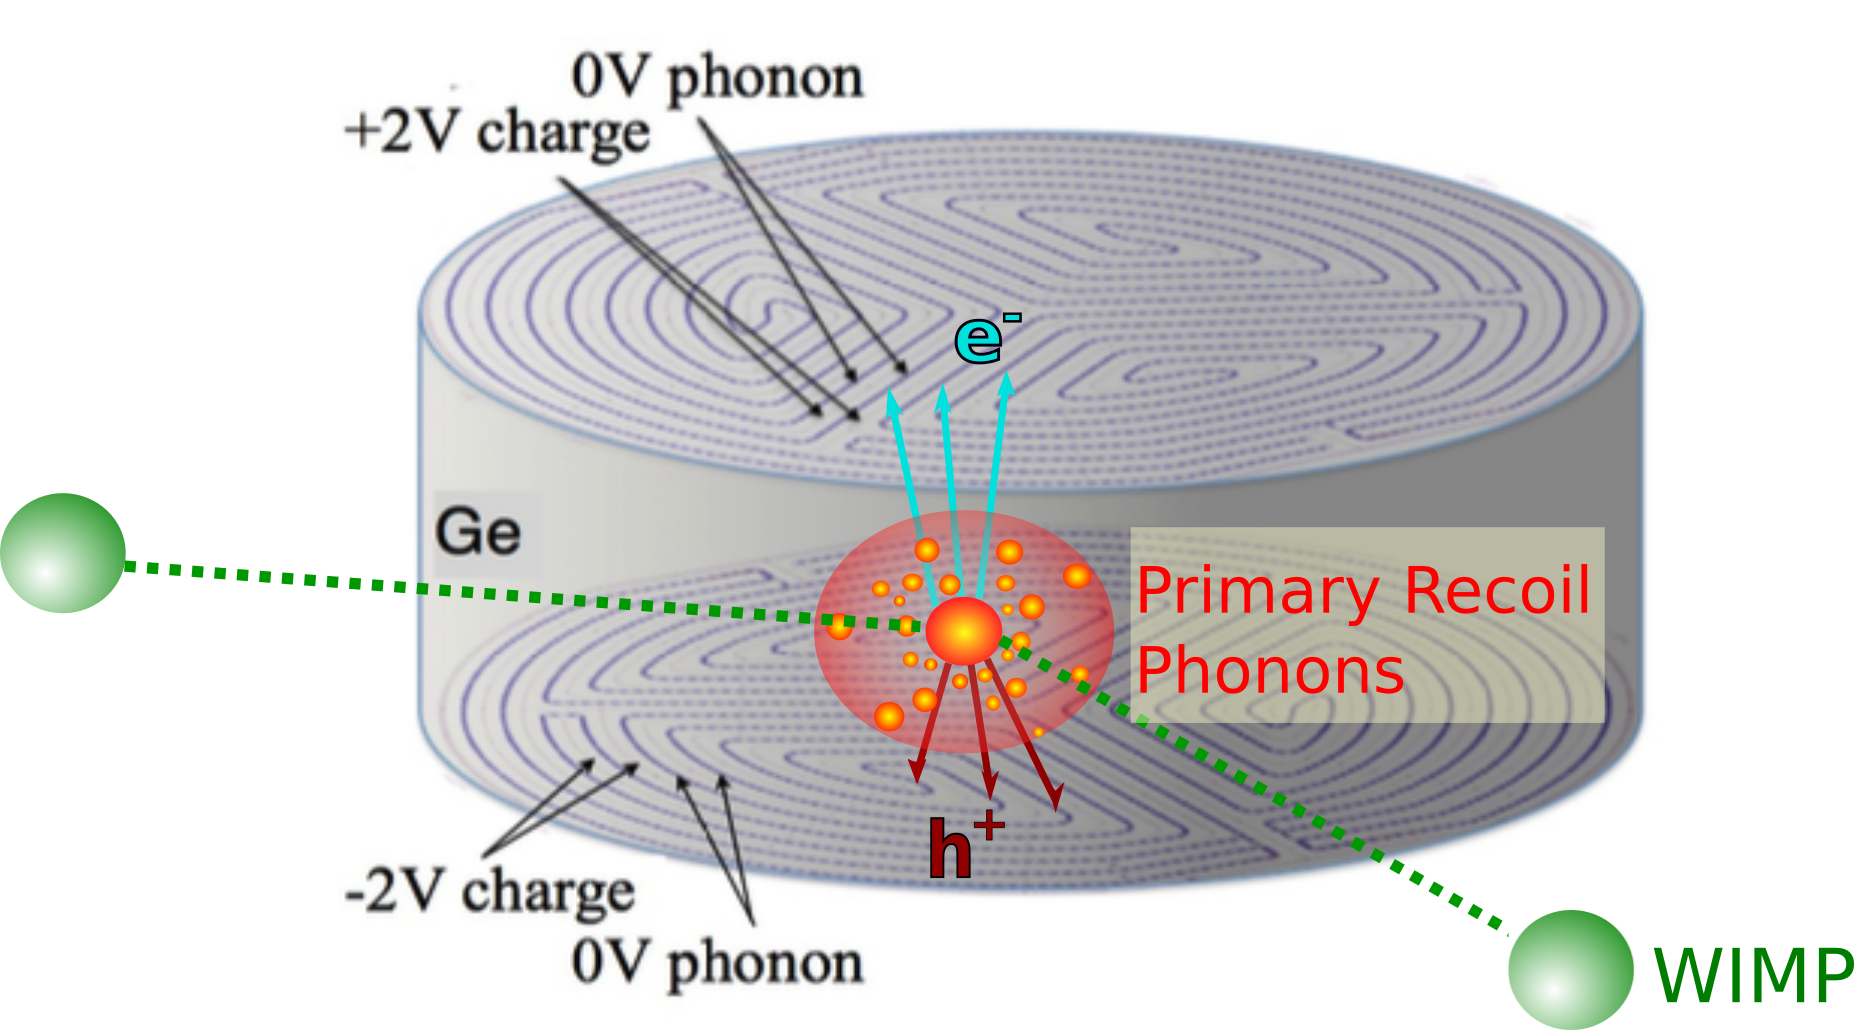
\includegraphics[width=0.9\linewidth]{Figures/iZIP.png}
\caption[iZIP Operating Mode]{iZIP operating mode. Electron-hole pairs produced by a particle scattering in the detector drift across the 4V bias to charge collectors on either detector face. The grounded phonon sensors measure the primary recoil phonons, and any additional phonons produced by the drifting electron-hole pairs. Reproduced from $\copyright$ \cite{SuperCDMS_Soudan}, with the permission of AIP Publishing.}
\end{figure}

The iZIP detectors employ two background rejection techniques, both of which are important for their sensitivity as dark matter detectors. The first is ionization yield discrimination, and the second is surface event rejection. Both are notably unavailable in the CDMSlite operating mode. 

\subsubsection{Ionization Yield Discrimination}

Ionization yield -- or simply ``yield" -- gives a measure of the total energy of electron-hole pairs ionized by a particle recoiling in the detector. It is quantified by the ratio of the measured ionization energy $E_\text{e/h}$ to the total energy $E_\text{r}$ of the recoil. SuperCDMS follows the conventional practice of calibrating the ionization energy scale such that this yield $Y=\frac{E_\text{e/h}}{E_\text{r}}$ is on average unity for electron recoils. 

By simultaneously collecting primary ionization and phonon signals, the iZIP detectors have the ability to measure the energy of a recoil event in the detector both in terms of the measured ionization energy $E_\text{e/h}$ and the  phonon energy $E_\text{p}$. The ionization energy is calibrated for electron recoils using peaks in the measured spectrum of electron recoil events from a $^{133}$Ba $\gamma$ calibration source. Using these same events, the phonon energy scale is calibrated relative to the ionization energy such that, after correcting for the Luke-Neganov gain discussed in Section 3.3.2, the resulting primary phonon energy measured for each event matches the calibrated ionization energy \cite{Fallows}:


\begin{equation}
Y=\frac{E_\text{e/h}}{E_\text{p}-\frac{eV_b}{\epsilon}E_\text{e/h}} \equiv 1 \text{ for electron recoil events}
\end{equation}

The term $\frac{eV_b}{\epsilon}E_\text{e/h}$ in the denominator represents the energy of the ``Luke-Neganov" phonons discussed further in Section 3.3.2, where $e$ is the absolute value of the fundamental electric charge, $V_b$ is the 4V bias across the detector, and $\epsilon$ is the energy required to ionize a single electron-hole pair.

The yield measurement is important for the sensitivity of iZIP detectors because it makes it possible to discriminate between nuclear recoils of interest for the WIMP search and the electron recoil background. Such discrimination is possible because nuclear recoil events have a significantly lower fraction of the initial recoil energy going into ionization compared with electron recoils, and can hence be distinguished from the electron recoil background by their lower ionization yield. Fig. 3.5 shows the discrimination between electron and nuclear recoil events based on the measured yield with data taken during activation of the detectors by a $^{252}$Cf $\gamma$ and neutron source.

\begin{figure}[H]
\centering
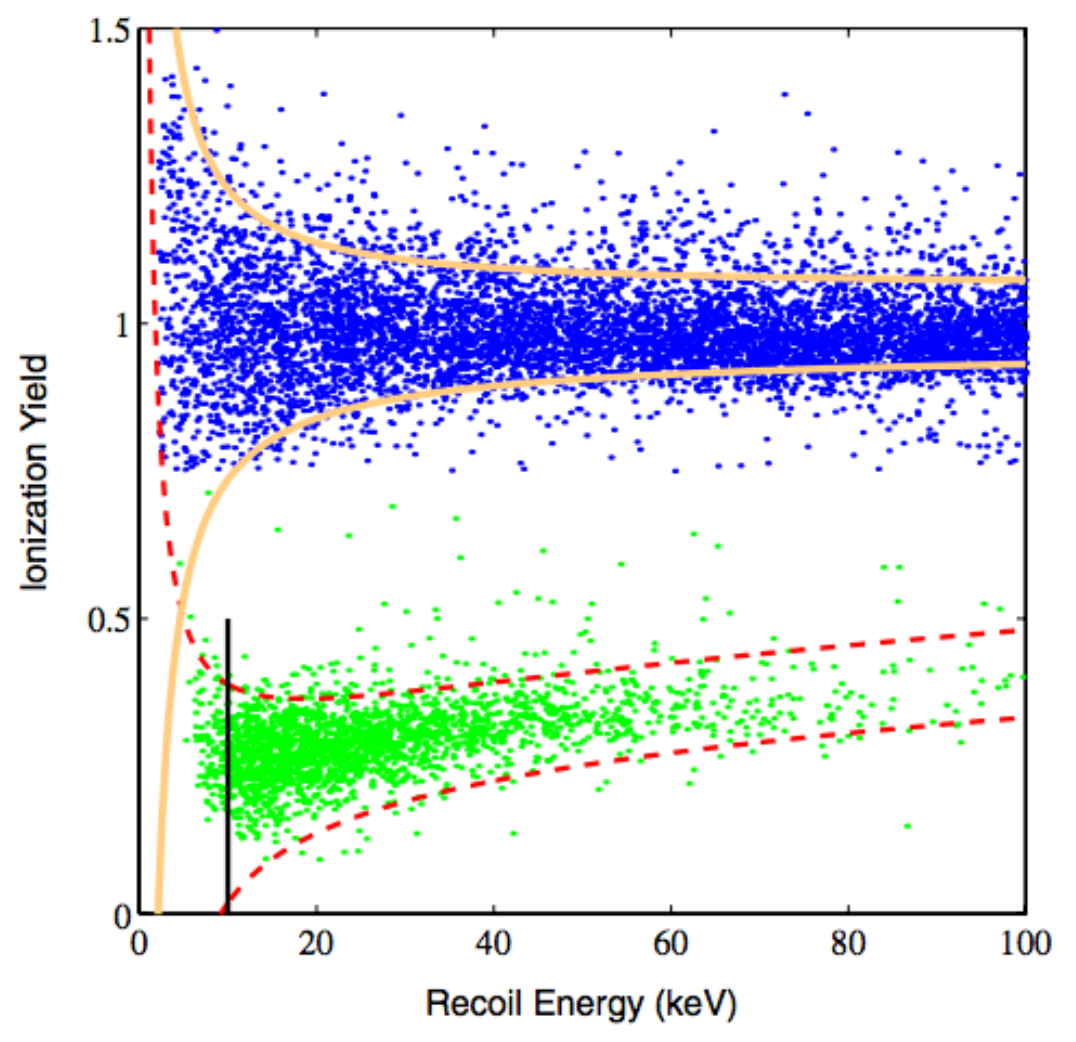
\includegraphics[width=0.5\linewidth]{Figures/YieldBands.png}
\caption[iZIP Ionization Yield Discrimination]{Discrimination between electron recoil (upper band) and nuclear recoil events (lower band) produced by $\gamma$ and neutron interactions, respectively, due to activation of an iZIP detector by a $^{252}$Cf $\gamma$ and neutron source. Reprinted figure with permission from \cite{Soudan_FirstResults}. Copyright (2004) by the American Physical Society.}
\end{figure}

\subsubsection{Surface Event Rejection}

As shown in Fig. 3.4, the phonon collectors (blue lines) and charge collectors (narrow grey lines) are interleaved in iZIP detectors, with a 1mm pitch \cite{SuperCDMS_Soudan}. The aluminum charge collectors are biased at +2V on one detector face and -2V on the other, and the phonon sensors are grounded. This interleaved pattern of phonon and charge collectors is an improvement over CDMS II detectors, which had phonon sensors on one side and charge sensors on the other \cite{SuperCDMS_Soudan}. The motivation for this improvement was to reject a background known as ``surface events". Surface events occur near the top and bottom of the detector, and represented a background in past generations of the experiment \cite{SuperCDMS_Soudan} because electronic carrier trapping at the surface prevented the full collection of their ionization signal \cite{mpyle}. This incomplete ionization collection made it possible to mistake the surface events for nuclear recoils due to the reduced ionization yield measurement.

\begin{figure}[H]
\centering
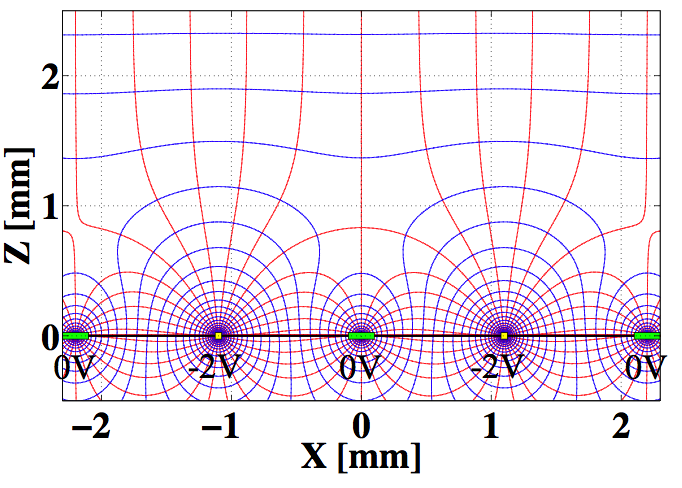
\includegraphics[width=0.6\linewidth]{Figures/SurfaceField.png}
\caption[iZIP Surface Electric Field]{Electric field near the surface of an iZIP detector produced by the pattern of interleaved biased charge collectors and grounded phonon collectors. Reprinted from \cite{SuperCDMS_Soudan}, with the permission of AIP Publishing.}
\end{figure}

The interleaved pattern of biased charge collectors and grounded phonon sensors addresses the surface event issue by creating the unique shallow electric field pattern shown in Fig. 3.6 in the first $\sim$2mm of the detector nearest the surface, while maintaining an approximately uniform electric field in the bulk of the detector. This surface field pattern ensures that an electron-hole pair created by an event near the detector surface is fully collected at that surface, with one charge collected at the biased electrode, and the other at the grounded phonon sensor. Since the otherwise uniform electric field ensures symmetric charge collection for electron-hole pairs created in the bulk of the detector, surface events can be identified and rejected by the absence of charge collected on the opposite detector surface. 

\subsection{CDMSlite Mode}

In the CDMSlite operating mode, the detectors are biased at 25-70V, much higher than is needed for full charge collection. The motivation for increasing the bias voltage is to take advantage of the ``Luke-Neganov" effect \cite{LukePhonon} to lower the energy detection threshold of recoil events in the detector, thereby extending the reach of CDMS detectors to lower WIMP masses. The lower energy threshold enables SuperCDMS to test extensions of the Standard Model that predict low-mass ($\sim$1-10 GeV/c$^2$) WIMP candidates \cite{CDMSlite_long}. The extended reach comes at a cost of sacrificing two significant background discrimination tools available to iZIP detectors, namely the yield discrimination and surface event rejection discussed in Section 3.3.1. 

\begin{figure}[H]
\centering
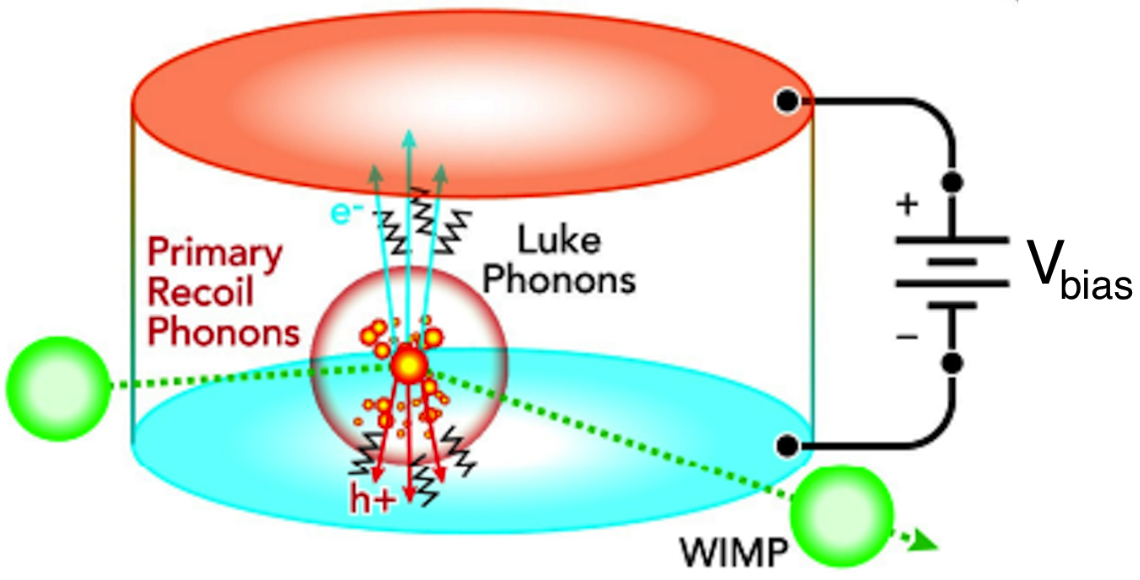
\includegraphics[width=0.6\linewidth]{Figures/CDMSlite.png}
\caption[CDMSlite Operating Mode]{CDMSlite operating mode. }
\end{figure}

\subsubsection{The Neganov-Luke Effect}

The CDMSlite operating mode achieves sensitivity to lower-energy recoil events than would be possible in iZIP mode because the relatively high bias voltage can amplify the primary -- and potentially sub-threshold -- ionization signal into a large measurable phonon signal. The phonon signal is a combination of the primary phonons produced by the recoil event, and ``Luke-Neganov phonons" emitted when the work done by the electric field in drifting the electron-hole pairs to the charge collectors is converted into thermal energy. 

The energy $E_\text{LN}$ of the Luke-Neganov phonons varies linearly \cite{LukePhonon} with both the number N of electron-hole pairs produced by the primary recoil event, and the bias voltage V$_b$ across the detector:

\begin{equation}
E_\text{LN}=NeV_b
\end{equation}

where $e$ is the absolute value of the fundamental electric charge. N, the average number of electron-hole pairs created, is given by:

\begin{equation}
N = Y\frac{E_r}{\epsilon}
\end{equation}

where Y is the ionization yield discussed previously in Section 3.3.1 and defined to be unity for electron recoils,  E$_r$ is the energy of the recoil event, and $\epsilon$ is the average energy required to produce a single electron-hole pair. $\epsilon$ is generally taken to be 3 eV / pair \cite{CDMSlite_long} for Ge.
%, though recent results \cite{MeiWei_epsilon} suggest that it could be as high as 3.32 eV. 
The total measurable phonon energy $E_\text{p}$ is hence:

\begin{equation}
E_\text{p}=E_r+E_\text{LN} = E_r\Big(1+Y\frac{eV_b}{\epsilon}\Big)
\end{equation}

The ionization yield Y for nuclear recoils, which will be discussed further in Chapter 4, has measured values within the range of 0.1-0.3 in the recoil energy range below 10 keV of interest for CDMSlite. At a nominal CDMSlite bias voltage of 70V, the ratio between the energy of the initial recoil event 
%- which is initially divided between primary electron-hole pairs and phonons - 
 and the energy of the Neganov-Luke phonons is $2.5 < \frac{70Y}{3} < 7$ for nuclear recoils. This has two important implications for the detector's WIMP sensitivity. First, it means that this operating mode can amplify the primary ionization signal of a WIMP-nucleon into a measurable phonon signal with up to 7 times the energy of the initial recoil event. Second, that the primary phonon signal is effectively overwhelmed by the larger Luke-Neganov phonon signal, making it impossible to calculate the ionization yield of the initial recoil event, and hence the yield-based discrimination between nuclear and electron recoil events available to iZIP detectors is not possible for CDMSlite detectors. 

\subsubsection{Data Acquisition Modifications for CDMSlite Operation}

Standard iZIP detectors were not designed to operate at a bias voltage above 10V, so detectors operated in CDMSlite mode are instrumented with custom electronics that keep one detector face at the desired operating voltage and the other detector face at ground \cite{CDMSlite}. The custom electronics at the biased detector face were not designed to read out signals, so all signal readout is done from the grounded detector face. The one-sided readout has the effect of both halving the total phonon signal, and making it impossible to employ the surface event rejection achieved by the two-sided iZIP-mode readout. This will not be a limitation at SNOLAB, where the high-voltage (HV) detectors will be instrumented with specialized electronics which will enable two-sided signal readout \cite{Projected_Sensitivity}.


\chapter{Photoneutron Calibration}

\section{Background and Motivation}

For a candidate WIMP-nucleon scatter event in a dark matter detector, the mass $m_\chi$ of the incident WIMP is calculable from the recoil angle $\theta_r$ and the energy E$_r$ of the recoiling nucleon (see Eq. 2.1). Therefore, an accurate determination of the recoil energy is needed to determine the distribution of possible WIMP masses that could have produced a candidate signal event. 

It is thus important to understand the relationship between the phonon energy detected by the TESs, and the recoil energy of the struck target nucleus. This relationship can be calibrated to $\sim2\%$ precision for electron recoil events in SuperCDMS detectors by passing $\gamma$ rays from a radioactive source such as $^{133}$Ba through the detectors and comparing peaks in the measured spectrum with known $\gamma$ lines from the source. However, the absence of characteristic peaks in neutron spectra makes such a calibration relatively difficult for neutron recoil events.

In principle, the phonon energy scale due to nuclear recoils can be related to the electron recoil scale according to Eq. 3.4, where the ionization yield Y defined in Section 3.3.1 is calibrated to unity for electron recoils. This calibration is described for iZIP detectors in Section 3.3.1. For CDMSlite detectors, the phonon energy scale is calibrated directly for electron recoils using peaks in spectra from a radioactive source, taking Y$\equiv$1 in Eq. 3.4. The nuclear recoil scale $E_\text{r,nr}$ is thus related to the electron recoil scale $E_\text{r,ee}$ according to:

\begin{equation}
E_\text{r,nr} = E_\text{r,ee}\frac{1+\frac{eV_b}{\epsilon}}{1+Y(E_\text{r,nr})\frac{eV_b}{\epsilon}}
\end{equation}

where $Y(E_\text{r,nr})$ is the energy-dependent ionization yield of a nuclear recoil event. The other terms in Eq. 4.1 are known, and described below Eq. 3.4. For iZIP detectors, $Y(E_\text{r,nr})$ can be measured directly at recoil energies above $\sim$10 keV$_\text{r,nr}$, as shown in Fig. 3.5. However, as discussed in Section 3.3.2, CDMSlite detectors have no ability to measure yield at all.
%, as the primary phonon signal is overwhelmed by Luke-Neganov phonons. 
Therefore, an independent determination of the ionization yield is required for the full CDMSlite nuclear recoil energy range, and below $\sim$10 keV for iZIP-mode detectors. This independent determination could come from theory, experiment, or a combination thereof. This chapter focuses on an experimental measurement of the CDMSlite nuclear recoil spectrum for SuperCDMS Ge detectors in the low-energy range of $\sim$0.4 to 10 keV$_\text{r,nr}$.

%, which according to Eq. 2.1 corresponds to an approximate range of 

%\begin{equation}
%\frac{m_\chi m_A}{m_\chi+m_A} = \sqrt{\frac{m_AE_r}{2v^2\cos^2\theta_r}} = \eta
%\end{equation}
%
%\begin{equation}
%m_\chi m_A = \eta(m_\chi+m_A) = \eta m_\chi + \eta m_A
%\end{equation}
%
%\begin{equation}
%m_\chi( m_A - \eta) = \eta m_A
%\end{equation}
%
%\begin{equation}
%m_\chi = \frac{\eta m_A}{m_A - \eta}
%\end{equation}

\subsection{Ionization Yield from Lindhard Theory}

Lindhard theory \cite{Lindhard_1963} provides a semi-empirical prediction for the ionization yield of a nuclear recoil $Y(E_\text{r,nr})$ as a function of nuclear recoil energy $E_\text{r,nr}$ for a material of mass number A and atomic number Z:

\begin{equation}
Y(E_\text{r,nr}) = k\frac{g(\epsilon)}{1+kg(\epsilon)}
\end{equation}

where:

$$g(\epsilon) = 2\epsilon^{0.15} + 0.7\epsilon^{0.6} + \epsilon$$
$$\epsilon = 11.5E_\text{r,nr}Z^{-7/3}$$

and the $k$ value from Lindhard theory is nominally given by:

\begin{equation} 
k_\text{nom} = 0.133Z^{2/3}A^{-1/2}
\end{equation}

which ranges from 0.156 to 0.160 for stable isotopes of Ge.

% averages to approximately 0.157 for natural Ge. 

\subsection{Existing Ionization Yield Data}

Existing measurements of the ionization yield -- also known as ``ionization efficiency" -- are shown for Ge in Fig. 4.1. With a few exceptions, the experimental measurements tend to agree with the Lindhard model prediction above $\sim$50 keV$_\text{r,nr}$, but begin to deviate significantly in the region near and below 10 keV$_\text{r,nr}$, resulting in a large uncertainty in the ionization yield in this low recoil energy range.

\begin{figure}[H]
\centering
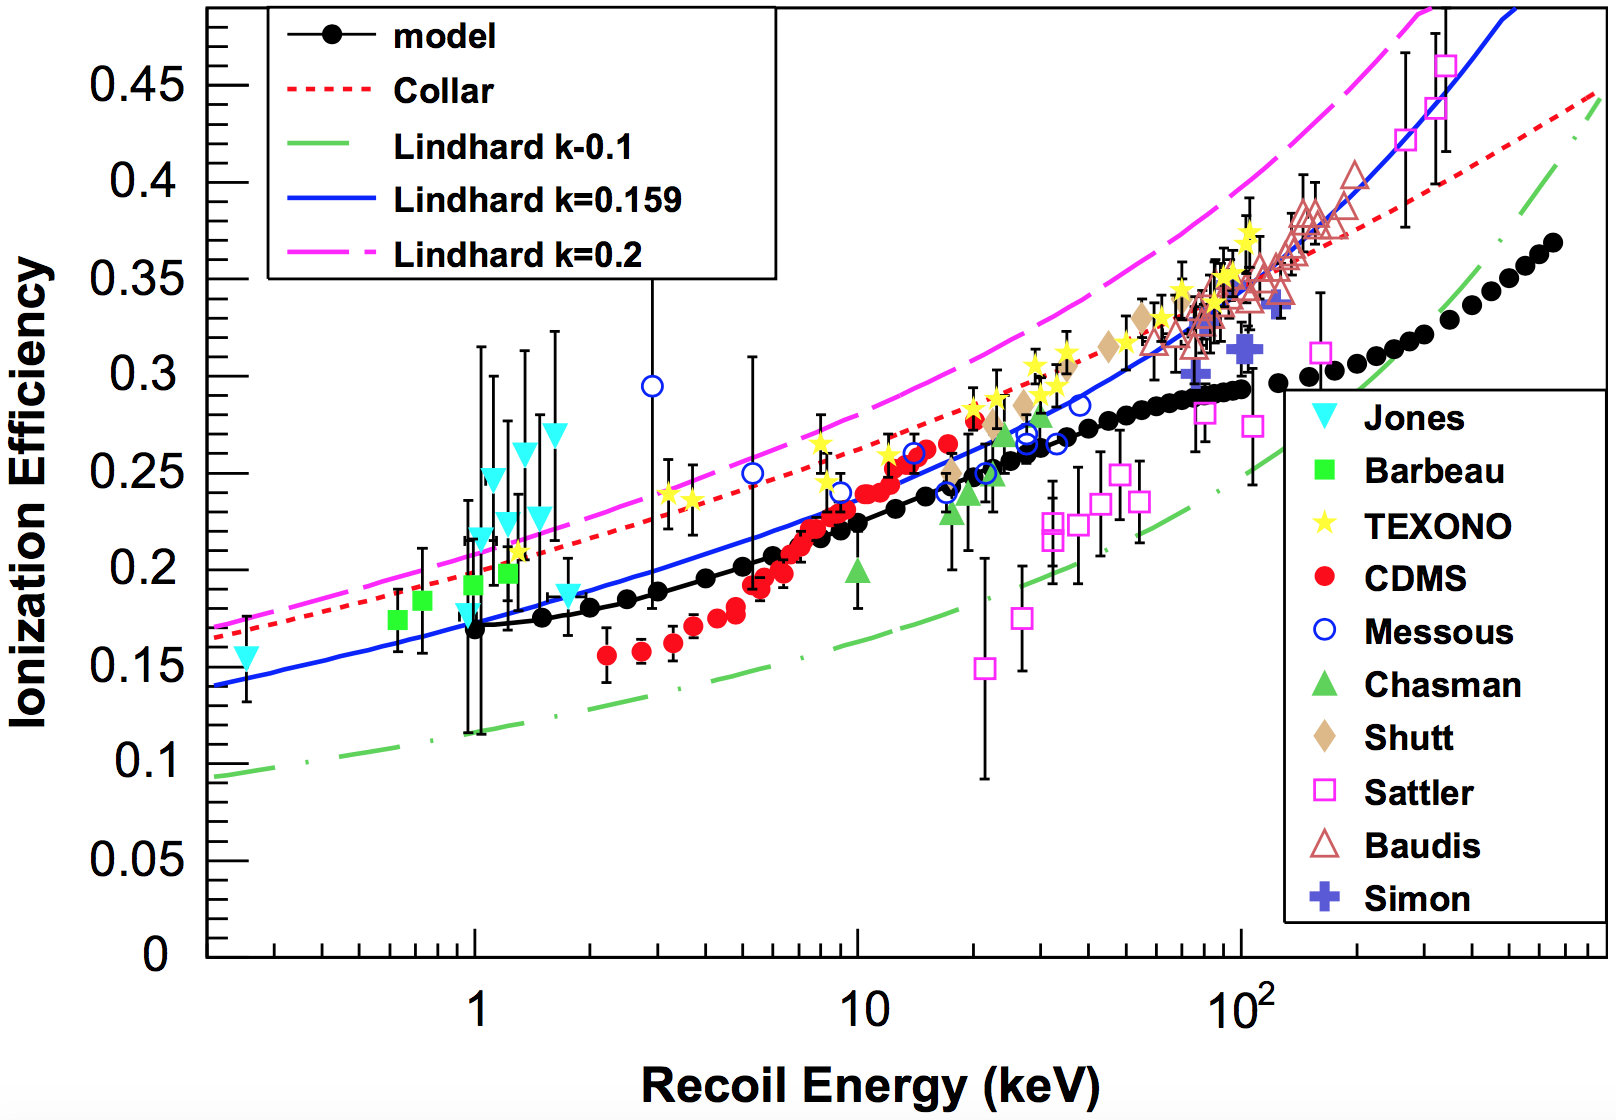
\includegraphics[width=0.8\linewidth]{Figures/IonizationYield.png}
\caption[Existing ionization yield measurements]{Existing ionization yield measurements. Measurements generally begin to agree with the Lindhard model, with $k\approx$0.159, above $\sim$50 keV$_\text{r,nr}$. Reprinted from \cite{Barker_Mei}, Copyright (2012), with permission from Elsevier.}
\end{figure}

The most recently published CDMSlite WIMP search using Run 2 data produced a world-leading limit on spin-independent WIMP-nucleon cross sections down to $\sim$3 GeV/c$^2$ \cite{CDMSlite_long} by pushing the low-energy noise threshold (discussed in Section 2.1.1) of the detectors down to nuclear recoil energies of $\sim$0.5 keV$_\text{r,nr}$. The upcoming installation of the SuperCDMS experiment at SNOLAB expects to further lower the noise threshold down to 0.04 keV$_\text{r,nr}$ \cite{Projected_Sensitivity} to probe WIMP masses as low as $\sim$0.5 GeV/c$^2$. However, determinations of the WIMP mass in this low energy region are limited by the large uncertainty in the ionization yield of Ge for nuclear recoil energies below $\sim$10 keV$_\text{r,nr}$. Previous and ongoing analyses of CDMSlite data use the Lindhard yield model, with $k$ in Eq. 4.2 allowed to range from 0.1 to 0.2 to account for the spread and uncertainty of existing yield data in the recoil energy range below $\sim$10 keV$_\text{r,nr}$. The resulting uncertainty in the energy scale dominates the uncertainty band on the WIMP-nucleon cross section limit, as shown in Fig. 4.2. The photoneutron calibration aims to constrain the low-energy ionization yield of SuperCDMS detectors, thus reducing the uncertainty on SuperCDMS sensitivity limits.

\begin{figure}[H]
\centering
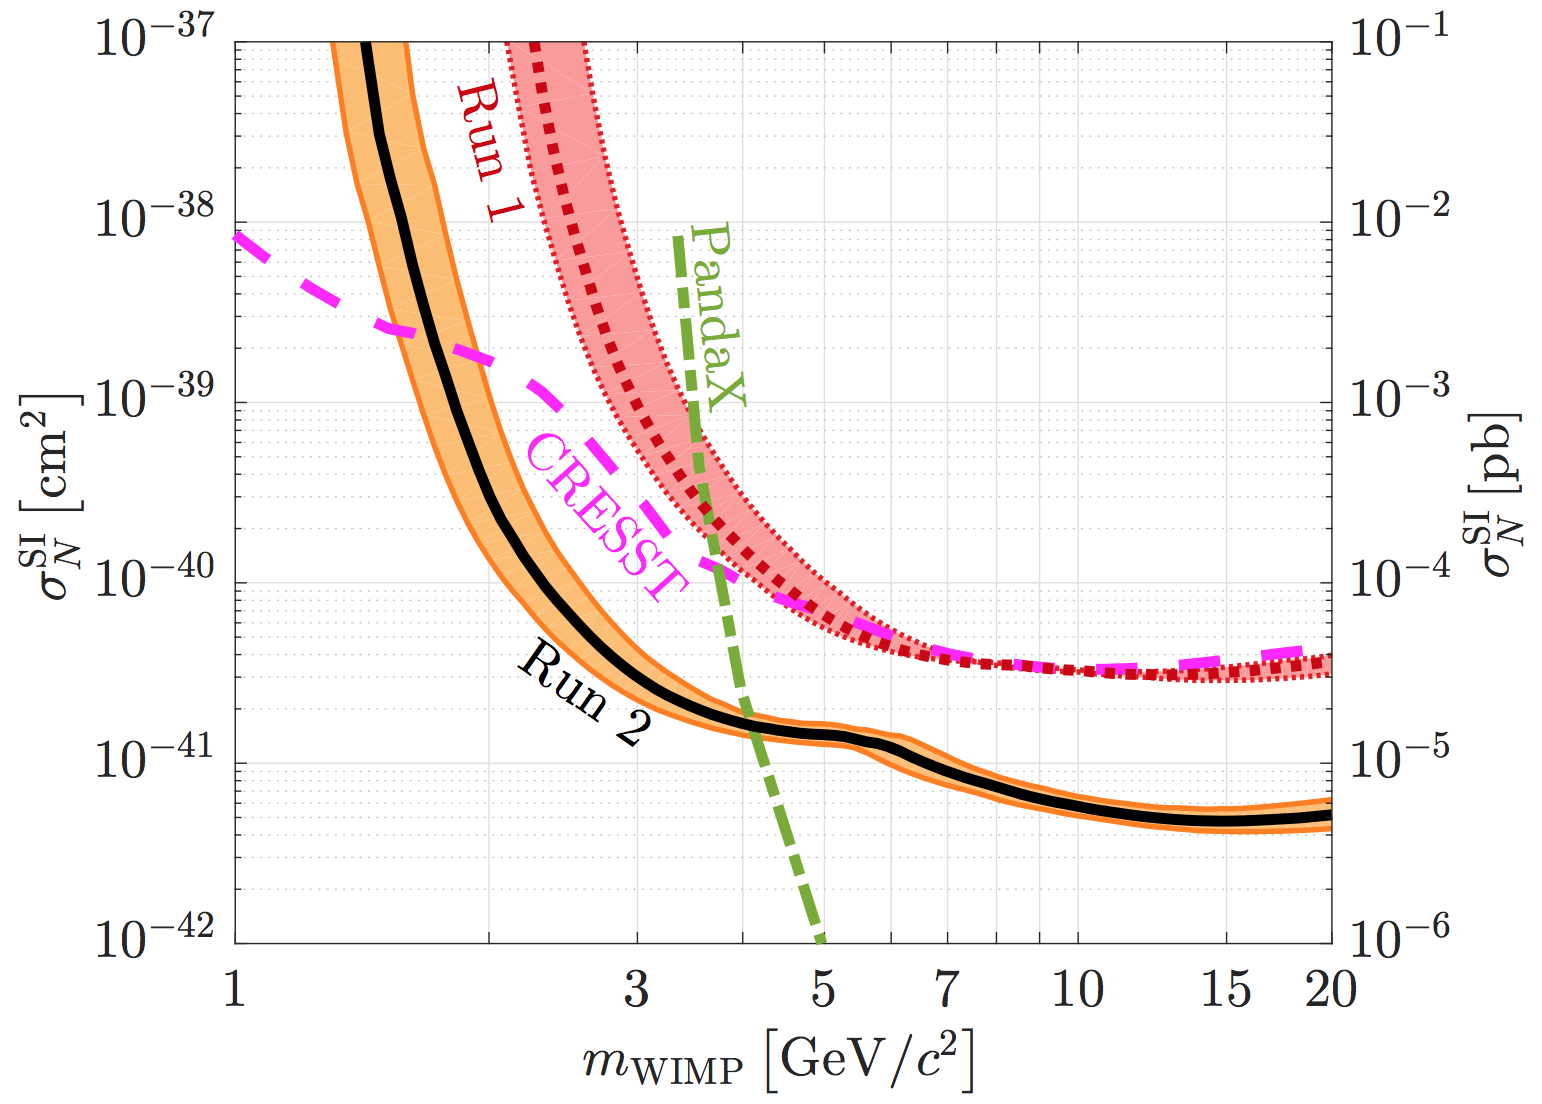
\includegraphics[width=0.8\linewidth]{Figures/R2_Limit.png}
\caption[Spin-independent WIMP-nucleon cross section limits from CDMSlite runs 1 and 2]{Spin-independent WIMP-nucleon cross section limits from CDMSlite runs 1 and 2, with uncertainty bands dominated by the energy scale uncertainty. Reprinted figure with permission from \cite{CDMSlite_long}. Copyright (2018) by the American Physical Society.}
\end{figure}

\section{Calibration Concept and Setup}

The concept of the photoneutron calibration is to pass approximately mono-energetic neutrons through SuperCDMS detectors, as illustrated in Fig. 4.3, and compare the resulting nuclear recoil spectrum, measured in phonon energy (keV$_t$), with a simulated nuclear recoil spectrum (measured in keV$_\text{r,nr}$) to calibrate the phonon energy scale. 

\begin{figure}[H]
\centering
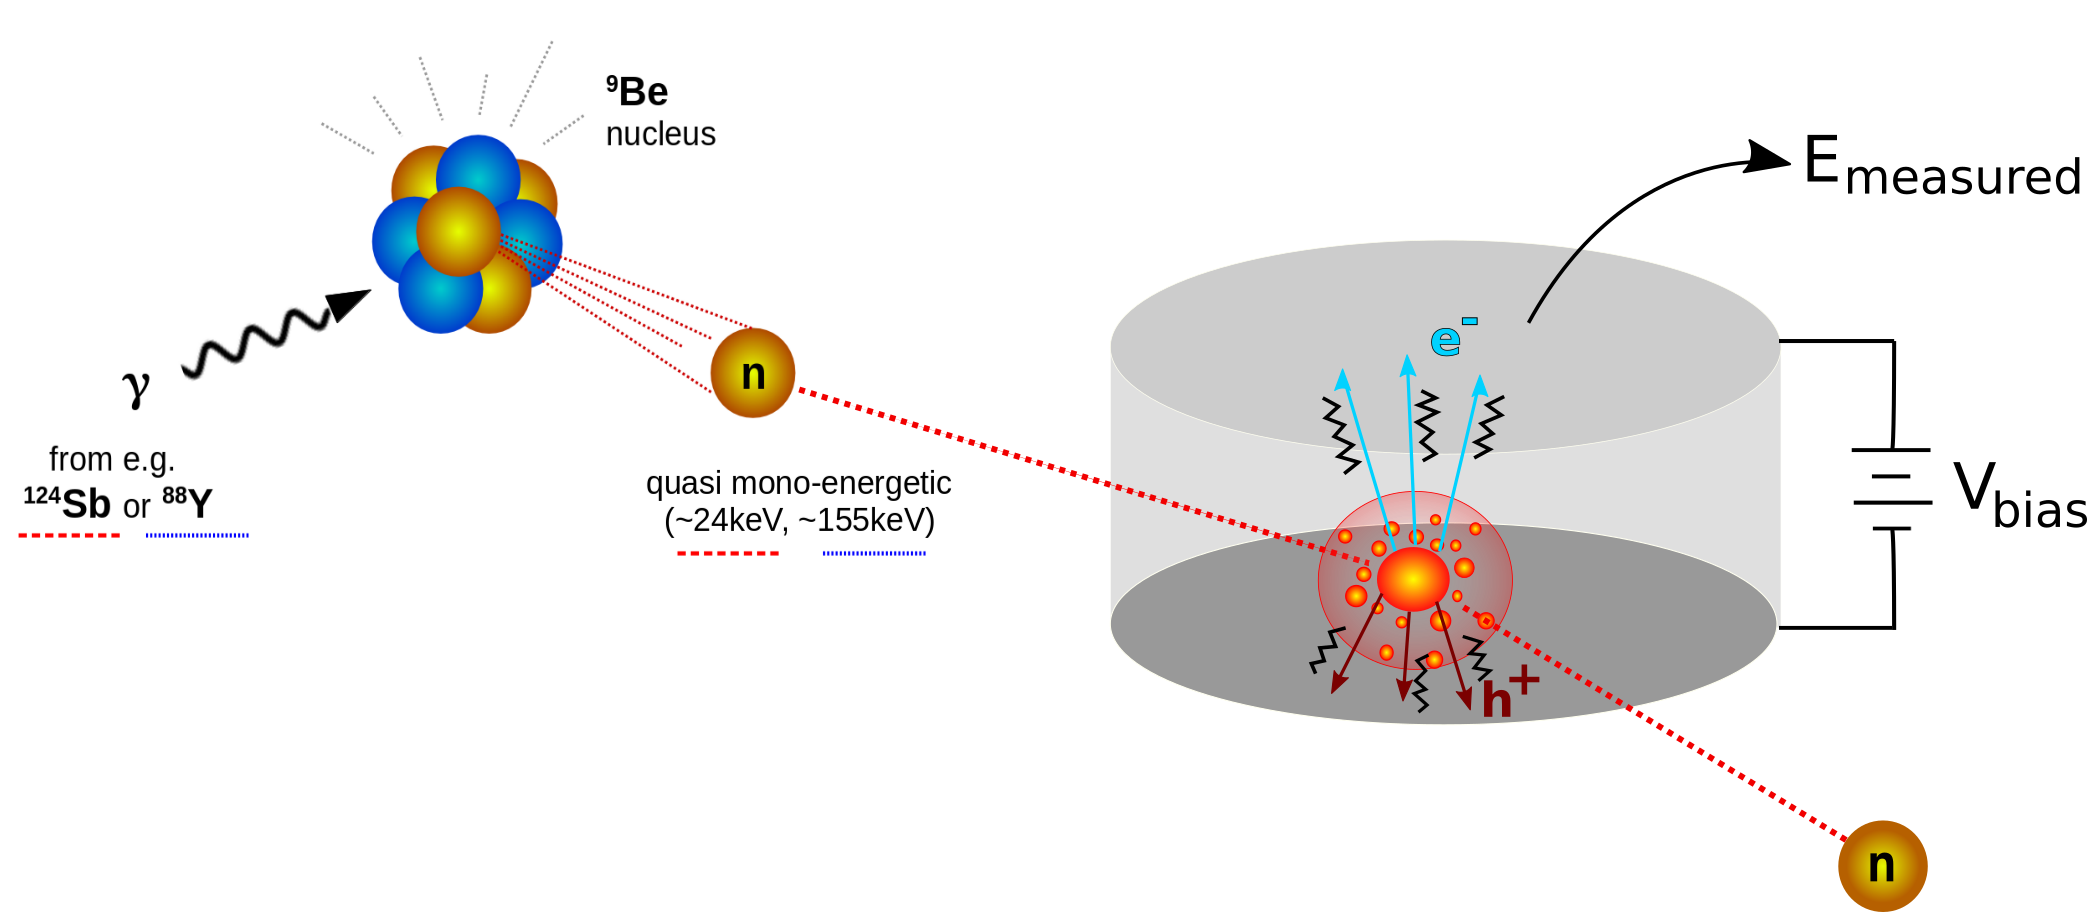
\includegraphics[width=0.9\linewidth]{Figures/CalibrationConcept.png}
\caption[Photoneutron calibration concept]{Photoneutron calibration concept}
\end{figure}

The neutrons are produced by passing $\gamma$ rays from a radioactive source -- either $^{124}$Sb or $^{88}$Y -- through a $^9$Be wafer. Due to the instability of the $^9$Be nucleus, incident $\gamma$ rays with energy $E_\gamma$ above the ``photoneutron production" threshold $E_\text{th}$=1.666 MeV \cite{Be_Threshold} of $^9$Be, and below 2.5 MeV \cite{Prosser_1960} can induce ``photo-disintegration" of the nucleus via a ($\gamma,n$) reaction. In this reaction, the absorption of the $\gamma$ ray by the nucleus is followed by the release of a neutron.

The energy of the emitted neutron is approximately mono-energetic, and given theoretically by \cite{Linac}:

\begin{equation}
E_\text{n} = \frac{A}{A-1}\Bigg[E_\gamma-E_\text{th}-\frac{E_\gamma^2}{(1862\text{ MeV})(A-1)}\Bigg]+\delta(\theta)
\end{equation}

where $A$ is the mass number of the target nucleus, and $\theta$ is the angle of the emitted neutron relative to the incident $\gamma$. $\delta_\theta$ represents the small angular dependence of the neutron energy, and is given by:

\begin{equation}
\delta_\theta = E_\gamma\Big[\frac{2(A-1)E_\gamma-E_\text{th}}{931A^3}\Big]^{1/2}\cos\theta
\end{equation}

In practice, the energy variation due to the angular term $\delta(\theta)$ can be minimized by allowing only a small solid angle to reach the detector. 

$^{124}$Sb has strong $\gamma$ lines above $E_\text{th}$ at 1.691 MeV (47.49\% absolute intensity) and 2.091 MeV (5.498\% absolute intensity), both of which contribute to photoneutron production.  $^{88}$Y has a single strong line at 1.8361 MeV. The $^{124}$Sb and $^{88}$Y sources are experimentally found \cite{Hanson_1949} to produce neutrons of energy 24$\pm$3 keV and 151$\pm$8 keV, respectively.

In principle, there should be a sharp and easily recognizable cutoff at the maximum kinetically allowable nuclear recoil energy given the energy of the incident neutrons, which could be used for calibration. This high-energy cutoff is visible in Fig. 4.4, in the dashed red ``single-scatter" component of the simulated nuclear recoil spectra developed for the analysis. However, given the size of the detectors, there is a reasonably high probability that a single incident neutron will induce multiple scatter events. This presents a problem, because the detector cannot in general resolve multiple scatter events, which means that the amplitude of a single pulse read out from the detector represents the sum of all energy depositions, and may add up to an energy greater than the kinematic cutoff. As such, the multiple scatter events have the effect of blurring the sharp spectral cutoff, as shown by the blue dashed ``multiple-scatter" component in Fig. 4.4. 

Instead of searching for a sharp cutoff, the nuclear recoil energy scale is calibrated as follows: a Geant4 simulation of the experimental setup, developed by another member of the analysis group, is used to generate a spectrum of recoil energies due to the neutron flux. The simulated spectrum is converted to phonon energy using a parameterized Lindhard model, and the resulting spectral shape is compared with that of the experimental spectrum to fit for optimized Lindhard model parameters, as described in Section 4.7.  

\begin{figure}[H]
\centering
\begin{minipage}{.5\textwidth}
  \centering
  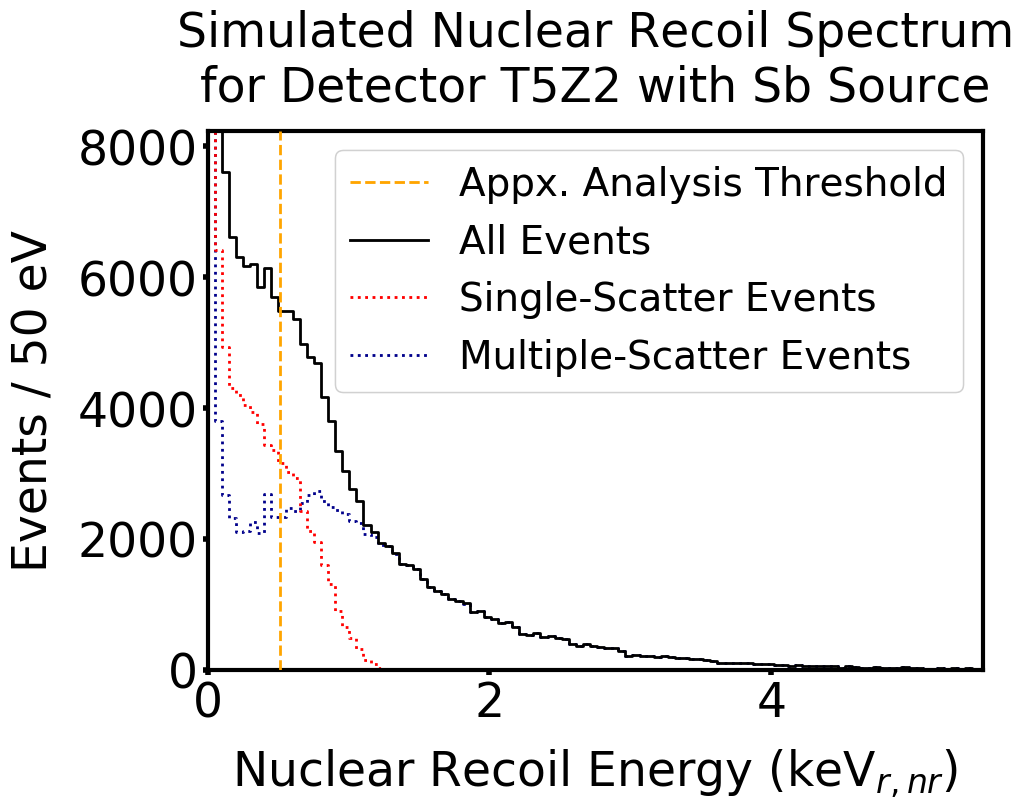
\includegraphics[width=.95\linewidth]{Figures/sb_70V_DetTypeCDMSlite_Simulation_Thesis.png}
%  \subcaption{}
\end{minipage}%
\begin{minipage}{.5\textwidth}
  \centering
  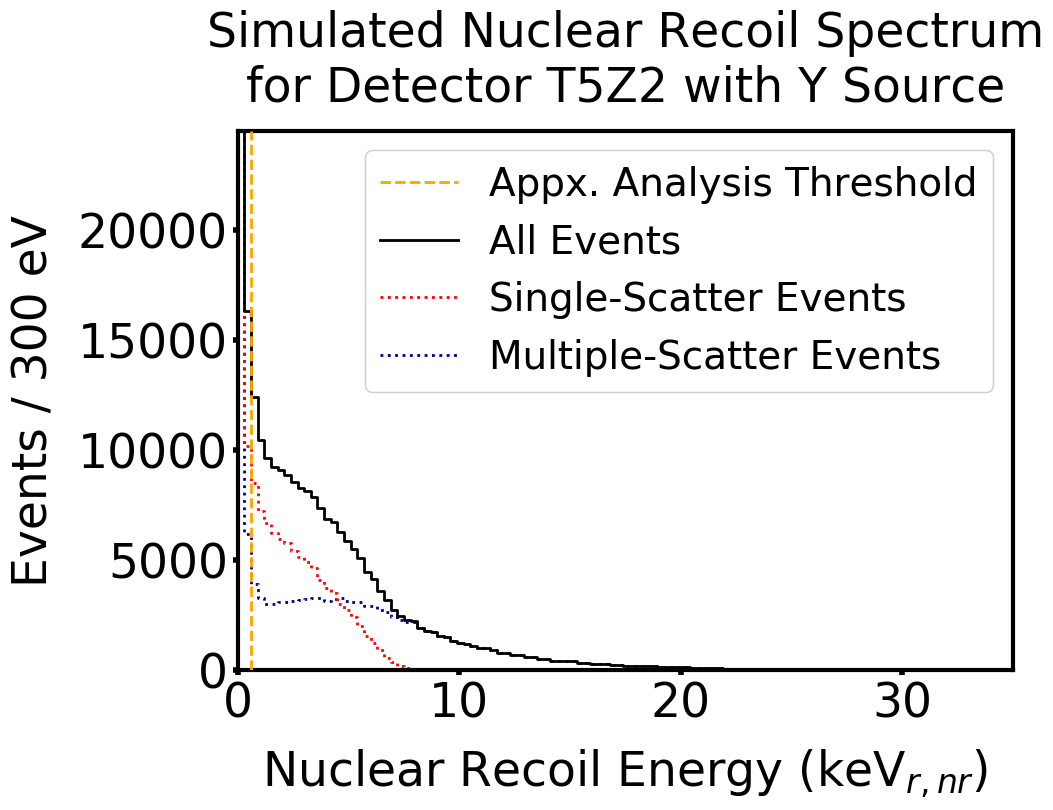
\includegraphics[width=.95\linewidth]{Figures/y_70V_DetTypeCDMSlite_Simulation_Thesis.png}
%  \subcaption{figure}
\end{minipage}
\caption[Dominant nuclear recoil component of the simulated neutron spectra for two of the three detector and source conditions used in the photoneutron calibration]{Dominant nuclear recoil component of the simulated neutron spectra for two of the three detector and source conditions used in the photoneutron calibration. Please see Fig. 4.32 left for a sample plot of the full neutron spectrum due to both nuclear and electron recoils.} 

%Red dashed: Component of the spectrum due to events for which the incident particle scatters only once in the detector. Blue dashed: Component due to events for which the incident particle scatters more than once. Black solid: Full nuclear recoil spectrum.}
\end{figure}

\section{Experimental Setup}

\subsection{Physical Setup}

The physical setup for the photoneutron calibration is illustrated by the simulated side-view in Fig. 4.5. The radioactive source is placed in a source holder above the vacuum cryostat containing the five towers of detectors, with a lead block immediately underneath to reduce the flux of $\gamma$ rays from the source. The vast majority of $\gamma$ rays pass through the wafer without interacting (on the order of one ($\gamma,n$) reaction per $\sim$10$^5$ $\gamma$s). For this reason, it was necessary to alternate the data-taking conditions between:

\begin{enumerate}[a)]
\item placing the $^9$Be wafer underneath the source to collect data with both the neutrons and the $\gamma$ background (i.e. ``neutron-on"), and
\item removing the wafer to collect data with the $\gamma$ background alone, which can be used for spectral subtraction (i.e. ``neutron-off").
\end{enumerate}

\begin{figure}[H]
\centering
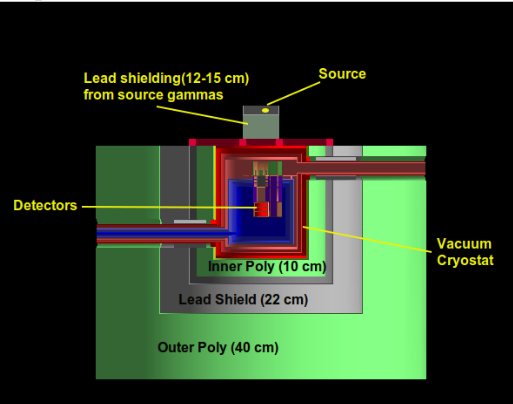
\includegraphics[width=0.6\linewidth]{Figures/ExpSetup.png}
\caption[Physical setup for the photoneutron calibration]{Physical setup for the photoneutron calibration}
\end{figure}

Preliminary studies found that, in the absence of the lead shielding, the deadtime-limited DAQ would be collecting nearly all $\gamma$s, and very few neutrons. The thickness of the lead shielding was thus optimized to reduce the flux of $\gamma$ rays to a manageable level without excessive degradation of the neutron spectrum due to neutrons interacting in the lead blocks. 

The veto panels, as well as the polyethylene and lead lids that are normally placed above the cryostat during WIMP search runs, were removed for the calibration, and mylar film was placed above the cryostat to prevent radon from seeping into it. 

The source holder is designed to contain the source and the optional $^9$Be wafer. The holder is mounted on top of several layers of lead shielding, on a source bridge above the outer vacuum cryostat. The source bridge is mounted on a translation stage (see Fig. 4.6 right) which offers one degree of translational freedom. 

\begin{figure}[H]
\centering
\begin{minipage}{.355\textwidth}
  \centering
  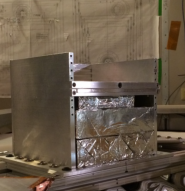
\includegraphics[width=.85\linewidth]{Figures/LeadShielding.png}
%  \subcaption{}
\end{minipage}%
\begin{minipage}{.645\textwidth}
  \centering
  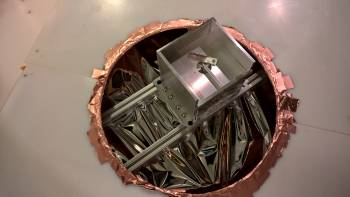
\includegraphics[width=.85\linewidth]{Figures/SourceBridge.jpeg}
%  \subcaption{figure}
\end{minipage}
\caption[Source box used to deploy the radioactive source]{Source box used to deploy the radioactive source. Left: Lead shielding is wrapped in aluminum foil and placed underneath the source. Right: The source box is mounted on a translation stage during data-taking.}
\end{figure}

The source is coupled to the end of a rod, which is screwed into a metal bar. The source can then be easily removed and replaced in a consistent location simply by unscrewing the bar that the rod is attached to, and later screwing it back into place (see Fig. 4.7 right). The source is placed directly above a circular hole that the $^9$Be wafer (the circular black wafer below the source in Fig. 4.7 left) can fit snugly into to collect neutron-on calibration data. 

\begin{figure}[H]
\centering
\begin{minipage}{.49\textwidth}
  \centering
  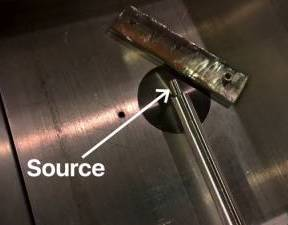
\includegraphics[width=.85\linewidth]{Figures/Source.jpeg}
%  \subcaption{}
\end{minipage}%
\begin{minipage}{.51\textwidth}
  \centering
  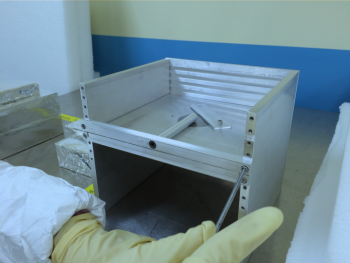
\includegraphics[width=.85\linewidth]{Figures/SourceScrew.png}
%  \subcaption{figure}
\end{minipage}
\caption[Radioactive source placement]{Radioactive source placement. Left: The source was placed on the end of a source rod, which was screwed into the source holder. Right: The source bar allows the source to be removed and replaced in a consistent location }
\end{figure}

\subsection{Data-taking Conditions}

The photoneutron data was taken over a 5 month period. Of the five towers of detectors in the vacuum cryostat, two were used to take data in CDMSlite mode for the photoneutron calibration: T2Z1 in Tower 2, and T5Z2 in Tower 5. There were three distinct data-taking conditions (i.e. ``data sets") used for CDMSlite-mode detectors:

\begin{itemize}
\item Operating detector T5Z2 at a 70V bias with the $^{124}$Sb source in place $\rightarrow$ \textbf{``Sb at 70V"}
\item Operating detector T5Z2 at a 70V bias with the $^{88}$Y source in place $\rightarrow$ \textbf{``Y at  70V"}
\item Operating detector T2Z1 at a 25V bias with the $^{88}$Y source in place $\rightarrow$ \textbf{``Y at  25V"}
\end{itemize}

Fig. 4.8 summarizes the periods during which each of the above three conditions were applied over the full course of the photoneutron calibration run.

\begin{figure}[H]
\centering
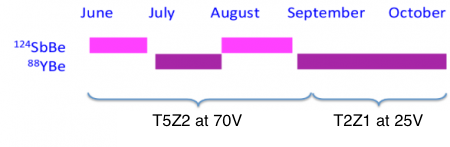
\includegraphics[width=0.8\linewidth]{Figures/Timeline.png}
\caption[Summary of data-taking periods for the photoneutron calibration]{Summary of data-taking periods for the photoneutron calibration}
\end{figure}

Each week of data-taking is divided approximately equally between:

\begin{enumerate}[a)]
\item placing the $^9$Be wafer beneath the source to collect data with both the neutrons and $\gamma$ background (known as ``neutron-on" data), and
\item removing the wafer to collect the $\gamma$ background alone (known as ``neutron-off" data).
\end{enumerate}

Data is collected in ``series" with nominal lengths ranging from 50 minutes to 3 hours. Each series is given a unique 11-digit identifier called a ``SeriesNumber", which encodes the following information:

\begin{itemize}
\item which facility the data was collected from (SuperCDMS has several test facilities in addition to the underground lab)
\item the time and date at which the series started.
\end{itemize}

\subsection{Trigger and readout settings}

For typical calibration runs with the source located above the detectors, the high interaction cross section makes it such that an incident particle is very likely to interact at least once in each of the three detectors in a tower. Therefore, traces and trigger bits are typically read out from all three detectors in the tower to determine the ``trigger threshold" for each detector -- i.e. the minimum measured recoil energy down to which a trigger in another detector in the tower is consistently accompanied by a trigger in the detector under consideration.

The high event rate produced by the $\gamma$ background motivated two atypical trigger and readout settings for the photoneutron data-taking: 

\begin{itemize}
\item Data was \textbf{not} taken in full-tower readout mode described above. Rather than collecting waveforms from every detector in the tower when a global trigger was produced, waveforms were only saved from the detectors that produced a trigger.
\item A high-energy (P$_\text{hi}$) trigger veto was applied in addition to the usual low-energy (P$_\text{low}$) trigger. The effect of this phi trigger was to prevent high-energy recoil events from being saved by the DAQ system, since the analysis is only interested in the relatively low-energy neutron spectrum below 10 keV$_\text{r,nr}$.
\end{itemize}

Since the absence of full-tower readout prevented a calculation of the trigger threshold using the photoneutron calibration data, this calculation was instead done using calibration data that had previously been taken with a $^{252}$Cf activation source. The trigger threshold was calculated for each detector by another member of the analysis group. 

\section{Cut Development}

\subsection{Basic Cuts}

Various ``basic cuts", summarized below, are applied to each data set to remove events that are considered unsuitable for the analysis. The basic cuts are characterized as being easily defined without the need for significant analysis or tuning.

\subsubsection{NotEmpty Cut}

For a given trigger or set of triggers produced by one or more of the detectors, the DAQ system decides, depending on the readout mode, which detectors to collect raw traces from for later processing. If a raw trace was not collected for a given event from the detector under consideration, this event is removed from the analysis of this detector using the NotEmpty cut.

\subsubsection{NotRandom Cut}

During each series, ``random" events -- or simply ``randoms" -- are periodically collected. Unlike typical saved events, these randoms do not correspond to a detector trigger. Randoms are used for data processing to evaluate the noise environment during each series. However, since they are not triggered by physical scatter events, they are removed from the analysis with the NotRandom cut.

\subsubsection{BaseTemp Cut}

The operating base temperature of the detectors lies in the approximate range of 35 to 55 mK. The base temperature is normally stored for each event, and may be used to make small corrections to the energy estimate. If the base temperature is not read out properly -- as signified by a value $\leq0$ -- its energy cannot be properly corrected. Such events are conservatively removed with the BaseTemp cut.

\subsubsection{High-Voltage Cut}

The energy scale of the detector varies with the bias voltage $V_b$ across the detector according to Eq. 3.4. Therefore, the analysis relies on an accurate, consistent bias voltage, so any events for which the voltage output reported by the power supply deviates from the nominal operating voltage are removed by the high-voltage cut.

\subsubsection{BiasFlashTime Cut}

Each data-taking run nominally begins by ``flashing" infrared LED light through the detector, which ``neutralizes" the detector crystal -- i.e. liberates charges that were trapped in crystal impurities. If the detector is not neutralized, electron-hole pairs produced by a recoil event may not be fully collected, which results in a reduced ionization yield estimate. The time during which a detector is biased following the most recent LED flash is recorded by the DAQ as the ``BiasFlashTime".  

The BiasFlashTime cut is designed to remove any events that were recorded after the nominal run length following the most recent detector flash, which could happen if the detector was for some reason not flashed before the next run. 

\subsubsection{Zero Current and Current Leakage Cuts}

It is expected that a small amount of leakage current (on the order of nA) will leak from the detector's voltage supply due to a parasitic resistance to ground. This leakage current is measured from the power supply and saved for each event. The leakage current reduces the bias voltage across the detector, and this effect is corrected for during processing when the energy of an event is estimated. 

As with the base temperature measurement, events for which the current leakage was not properly readout -- as signified by a leakage current of 0 -- will not have been properly corrected, and are therefore removed by the zero current cut.

Events with an excessive amount of leakage current -- where the excess appears to be associated with collecting data too soon after the last LED flash -- are removed with the current leakage cut, with a maximum allowable leakage of 3.0 nA.

\subsection{Quality Cuts}

Quality cuts require some degree of analysis and tuning. These cuts are described below, with particular emphasis on the cuts or aspects of cuts that I developed.

\subsubsection{Pre-pulse Standard Deviation Cut}

Raw phonon pulse traces, with a total length of 6553.6 $\mu$s, include $\sim$950 $\mu$s prior to the trigger. This ``pre-pulse region" is used during processing to calculate the pre-pulse standard deviation, which provides a measure of the noise level in the detector at the time of the pulse. 

A pre-pulse standard deviation cut is applied individually to each week of neutron-on and neutron-off data to remove data for which the pre-pulse standard deviation in any of the four phonon channels varies too strongly from the typical value. 

For each week of neutron-on or neutron-off data, the distribution of pre-pulse standard deviations in each phonon channel (A, B, C, and D) is fit with a Gaussian distribution, as shown in Fig. 4.9, and any events lying more than four standard deviations away from the centroid of the Gaussian fit in any of the four phonon channels are removed from the analysis.

\begin{figure}[H]
\centering
  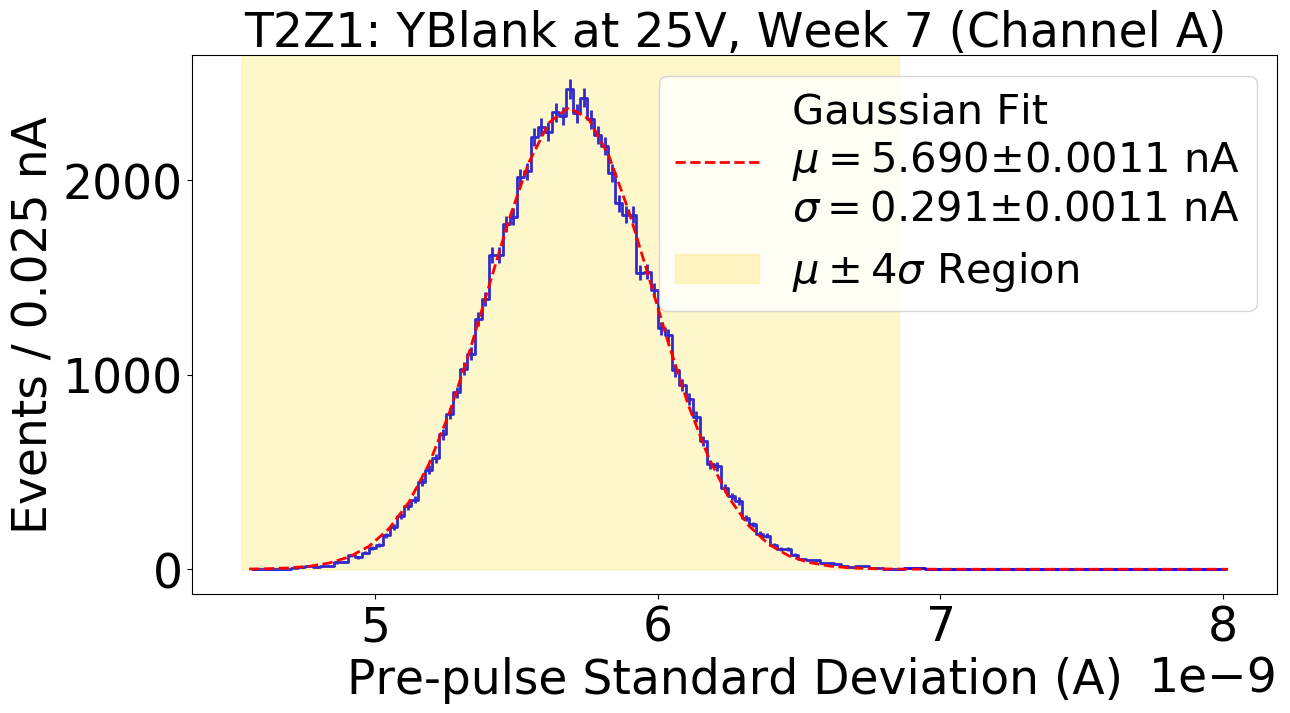
\includegraphics[width=0.6\linewidth]{Figures/Pstd_Thesis.png}
%  \subcaption{}
\caption[Sample application of the pre-pulse standard deviation cut]{Sample application of the pre-pulse standard deviation cut. A Gaussian distribution is fit to the distribution of pre-pulse standard deviations in phonon channel A for a sample week of the neutron-off Y data (i.e. ``YBlank"). Data lying more than $\pm4\sigma$ from the centroid of the Gaussian distribution is removed by the cut.}
%Right: Location of the cut for all weeks of neutron-off ``Y at 25V" data, shown as black horizontal lines 4$\sigma$ above and below the main distribution.}
\end{figure}

\subsubsection{Phonon Good Start Time (i.e. Phonon Delay) Cut}

The reconstructed start-time of an event is calculated as the optimized time delay (i.e. ``phonon delay") relative to the global trigger obtained when the raw phonon trace is fit to a phonon pulse template using the ``optimal filter" (OF) fitting method. The Phonon Good Start Time cut is designed to eliminate events whose reconstructed start-time occurs too close to the edges of the allowable OF search window to accurately measure the pulse. The OF search window ranges from -200$\mu$s to +100$\mu$s relative to the global trigger.

The cut, shown for the Sb at 70V data set in Fig. 4.10, is defined as:

\begin{equation}
\nonumber
-195\mu\text{s} < \text{phonon delay} < 35\mu\text{s}
\end{equation}

Note that the asymmetry in terms of the proximity of the upper and lower cutoffs to the OF search window edges arises from the fact that most of the portion of the pulse relevant for the OF fitting algorithm occurs after the reconstructed start-time.

\begin{figure}[H]
\centering
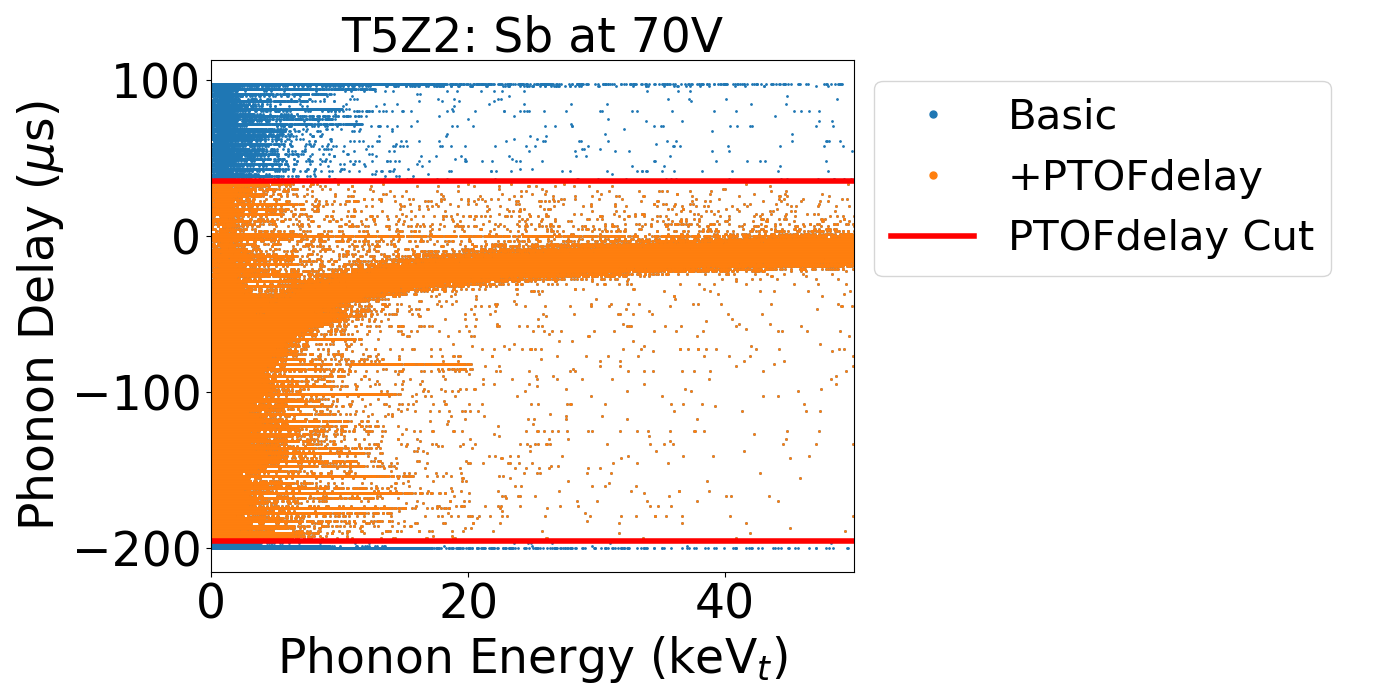
\includegraphics[width=0.7\linewidth]{Figures/PTOFdelay_vs_ptNF_DetCDMSlite_sb_70V_Thesis.png}
\caption[Sample application of the PTOFdelay cut]{Sample application of the PTOFdelay cut to data taken with the $^{124}$Sb source at a 70V bias (i.e. Sb at 70V). The upper and lower cut bounds are shown as red horizontal lines. Data passing the basic cuts described in Section 4.4.1 is shown in blue, and data additionally passing the phonon delay cut is shown in orange.}
\end{figure}

\subsubsection{Phonon Pulse Shape Cuts}

The phonon pulse shape cuts are comprised of three cuts that make use of $\chi^2$ estimates obtained from fitting each event's phonon pulse trace to one of three pulse templates during processing. These $\chi^2$ estimates are summarized as follows:

\begin{itemize}
\item \textbf{Phonon $\chi^2$ ($\chi^2_p$)}: Based on the fit to the ``good" signal pulse template, from which the best-fit pulse amplitude is used to obtain the phonon energy estimate. 
\item \textbf{Glitch $\chi^2$ ($\chi^2_g$):} Uses the ``glitch" pulse template, which is designed to represent pulses produced by electronic glitches in the detector readout electronics, rather than true signal events. This template is produced by averaging many pulses identified as electronic glitches, and is much more sharply peaked than the good signal pulse.
\item \textbf{LFN $\chi^2$ ($\chi^2_{lf}$):} Uses the ``low frequency noise" (LFN) pulse template. This template is designed to represent pulses produced by or contaminated with persistent LFN in the detectors. 
%The LFN has been found to be correlated with activity of the cryo-cooler in the dilution refrigerator. 
As with the glitch template, the LFN template is obtained by averaging many pulses identified with low-frequency noise. The LFN is particularly problematic near the low-energy trigger threshold. In this region, the vast majority of triggered events are due to LFN, resulting in what's known as the ``low-frequency noise blob".
\end{itemize} 

My primary involvement in the phonon pulse shape cuts was the development of ``time blocks" in which the $\Delta$Glitch and $\Delta$LFN cuts are most appropriately defined. Table 4.1 briefly summarizes the methodology used to define the cuts within each time block.

\begin{table}[H]
\centering
\caption[Summary of phonon pulse shape cuts defined within time blocks]{Summary of phonon pulse shape cuts defined within time blocks.}
\label{my-label}
\begin{footnotesize}
\renewcommand{\arraystretch}{1.5}
\begin{tabular}{|p{12mm}|L{25mm}|L{30mm}|L{50mm}|}
\hline
\textbf{Cut} & \textbf{Quantities Used for Definition} & \textbf{Purpose} & \textbf{Summary}  \\ \hline
Phonon $\chi^2$ & $\chi^2_p$, Total Phonon Energy ($E_p$) 	&  Identify instrumental background or pileup events based on a poor fit to the phonon pulse shape template, as indicated by a high $\chi^2_p$.   & For each data set (Sb at 70V, etc.), data is binned in $E_p$. In each $E_p$ bin, the cumulative density function (CDF) is computed in $\chi^2_p$, to obtain the 97\% CDF point. These 97\% CDF points are fit with a third-order polynomial to obtain an energy-dependent upper bound on $\chi^2_p$.              \\ \hline
$\Delta$Glitch       & $\Delta$Glitch$\equiv(\chi^2_g-\chi^2_p)$, $E_p$    &  Identify instrumental background events arising from electronic glitches, as indicated by a relatively good fit to the glitch template compared with the good phonon template.  	&  Within each time block, the data is binned in energy. In each bin, the mean and RMS values of $\Delta$Glitch are calculated, and the mean + 2.58$\times$(RMS) points are fit with a parabola to obtain an energy-dependent upper bound on $\Delta$Glitch. A flat cut in $\Delta$Glitch is also placed to minimize the contribution from the low-frequency noise blob.               \\ \hline
$\Delta$LFN      &  $\Delta$LFN$\equiv(\chi^2_{lf}-\chi^2_p)$, $E_p$  & Identify instrumental background events arising from low-frequency noise, as indicated by a relatively good fit to the LFN template compared with the good phonon template.  & Within each time block, the procedure is analogous to that used to define the $\Delta$Glitch cut.               \\ \hline
\end{tabular}
\end{footnotesize}
\end{table}

The phonon pulse shape cut definitions described in Table 4.1 were developed by another member of the analysis group.

%, and will be used to obtain the final analysis result. However, these cuts were not quite ready to use in time for inclusion in this thesis. Instead, the analysis presented in this thesis uses relatively loose quadratic Phonon $\chi^2$ and $\Delta$Glitch cuts that I defined within entire data sets to remove events clearly above the main distribution and within the low-frequency noise blob in the neutron-off data. These preliminary cuts are defined as:
%
%\textbf{Phonon $\chi^2$:}
%\begin{equation}
%\nonumber
%\text{Phonon }\chi^2 < a_2E_p^2 + a_0
%\end{equation}
%
%\textbf{$\Delta$Glitch:}
%\begin{equation}
%\nonumber
%\Delta\text{Glitch}  < b_2E_p^2 + b_0
%\end{equation}
%
%where the coefficients are listed for each data set in Table 4.2, and Fig. 4.11 shows the cuts for the Y at 70V data set. 
%
%The motivation behind the choice of preliminary cut locations is analogous to that of the finalized cut -- i.e. to remove events that lie above the main distribution in the Phonon $\chi^2$, $\Delta$Glitch, and $\Delta$LFN quality planes. The main difference is that this  effect is achieved by-eye with the preliminary cuts by visually locating the main distribution and removing events in the sparse region above it, whereas the finalized cuts employ the more systematic approach described in Table 4.1. As shown in the bottom left plot of Fig. 4.11, the Phonon $\chi^2$ cut effectively removes all events that lie significantly above the main distribution for energies above the low-frequency noise blob (i.e above $\sim$ 10 keV$_t$). Therefore, the primary purpose of the $\Delta$Glitch cut is to remove any noise blob events missed by the Phonon $\chi^2$ cut that are not degenerate with the main distribution of $\Delta$Glitch vs. phonon energy. Since the noise blob is more effectively separated from the main distribution in the $\Delta$Glitch plane compared with the $\Delta$LFN plane (see Fig. 4.11 right), the Phonon $\chi^2$ and $\Delta$Glitch cut were considered sufficient to achieve the goals of these preliminary cuts, without the need for an additional cut in $\Delta$LFN space.
%
%
%\begin{table}[H]
%\centering
%\caption[Summary of parabolic coefficients for preliminary pulse shape cuts used in this thesis]{Summary of parabolic coefficients for preliminary pulse shape cuts used in this thesis.}
%\label{my-label}
%\begin{footnotesize}
%\renewcommand{\arraystretch}{1.5}
%\begin{tabular}{|p{20mm}|L{15mm}|L{15mm}|L{15mm}|L{15mm}|}
%\hline
%\textbf{Data Set} & $a_2$ & $a_0$ & $b_2$ & $b_0$  \\ \hline
%Sb at 70V & 0.015  &   4800   & -4 & 15            \\ \hline
%Y at 70V & 0.015  &   5000   &  -3  & 15            \\ \hline
%Y at 25V & 0.002  &   4800   & -4 & 15            \\ \hline
%\end{tabular}
%\end{footnotesize}
%\end{table}
%
%\begin{figure}[H]
%\centering
%\begin{minipage}{\textwidth}
%  \centering
%  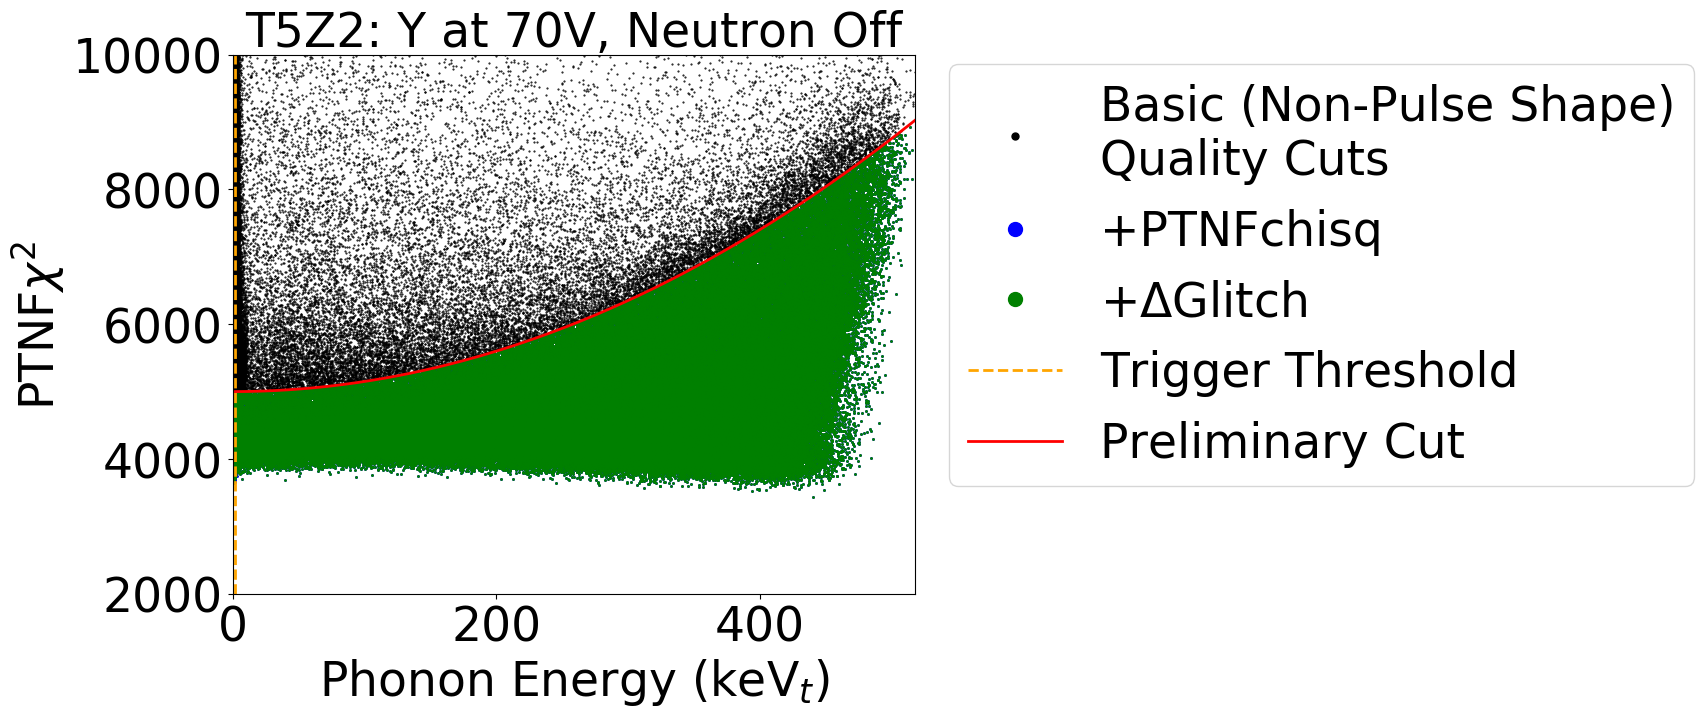
\includegraphics[width=0.9\linewidth]{Figures/DetCDMSlite_y_70V_PTNFchisq_Thesis.png}
%%  \subcaption{figure}
%\end{minipage}
%
%\begin{minipage}{.5\textwidth}
%  \centering
%  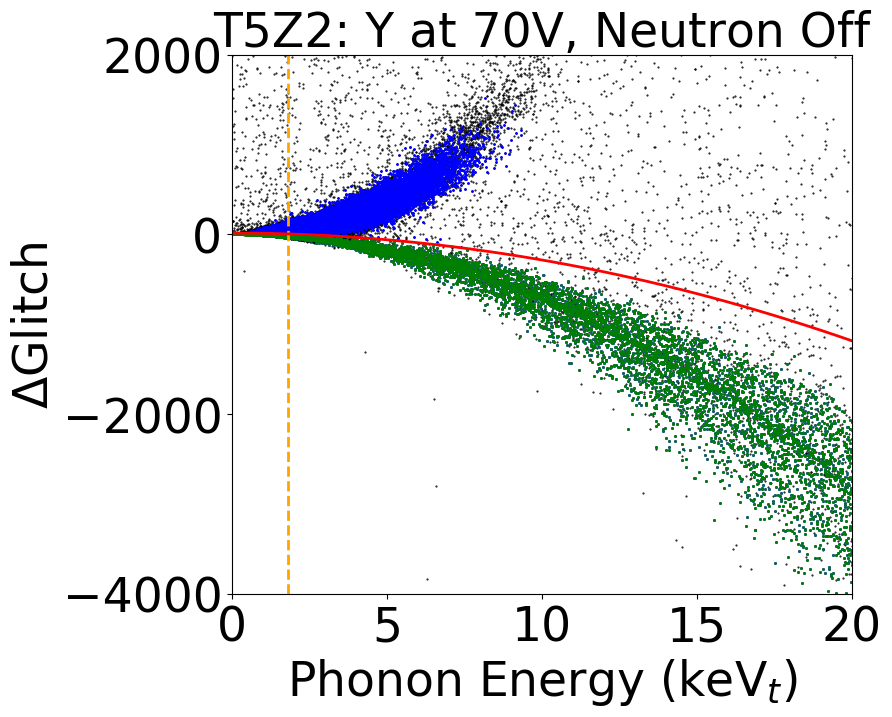
\includegraphics[width=0.95\linewidth]{Figures/DetCDMSlite_y_70V_Glitch_zoom_Thesis.png}
%%  \subcaption{}
%\end{minipage}%
%\begin{minipage}{.5\textwidth}
%  \centering
%  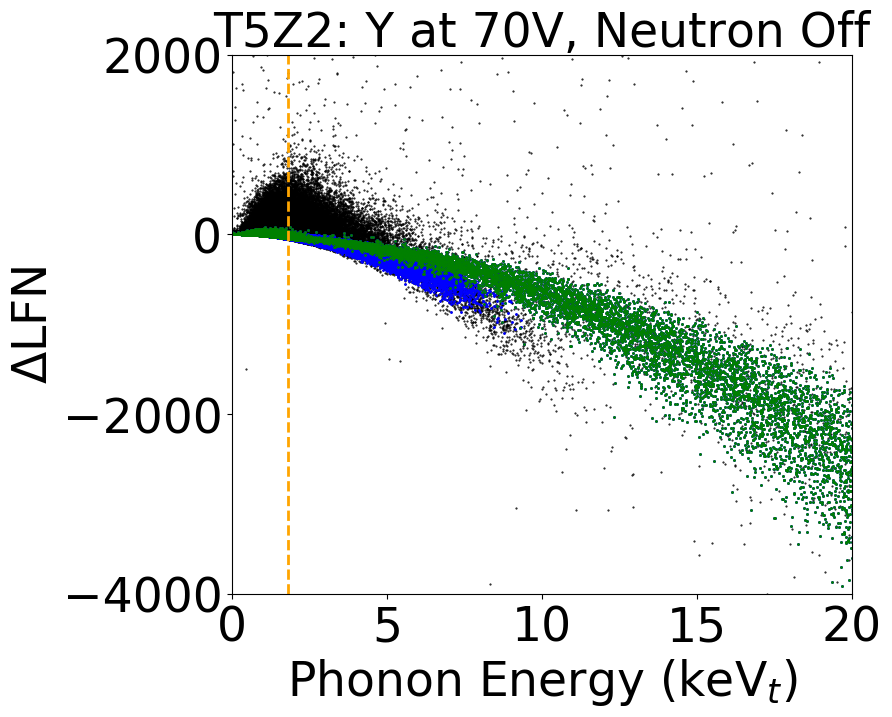
\includegraphics[width=0.95\linewidth]{Figures/DetCDMSlite_y_70V_LFN_zoom_Thesis.png}
%%  \subcaption{figure}
%\end{minipage}
%\caption[Effects of the preliminary pulse shape cuts in the phonon pulse shape vs. phonon energy planes for the Y at 70V dataset]{Effects of the preliminary pulse shape cuts in the phonon pulse shape vs. phonon energy planes for the Y at 70V dataset. The Phonon $\chi^2$ and $\Delta$Glitch cuts are shown as red lines in the top and bottom left plots, respectively. The blue and green points in each plot show the events remaining after respective application of the Phonon $\chi^2$ and $\Delta$Glitch cuts.}
%\end{figure}

The remaining discussion in this section will pertain to the development of the time blocks within which the finalized $\Delta$Glitch and $\Delta$LFN cuts are defined.

\textit{Time Block Development for the $\Delta$Glitch and $\Delta$LFN Cuts}

As described in Table 4.1, the $\Delta$Glitch and $\Delta$LFN cuts are defined to remove outliers for which these respective quantities lie beyond a certain percentile above the main distribution. It is known from previous SuperCDMS analyses that the detector noise environment can vary over time. Since the noise level, as measured on a series-by-series basis using series randoms, is used during processing in computing the $\chi^2$ quantities, a time variation in the measured noise environment can result in a time variation in typical $\chi^2$ estimates. It is therefore important to define these $\chi^2$ cuts within time blocks during which the location of the main distribution does not shift significantly in terms of these quantities. Otherwise, the cut will effectively be much harsher in some periods than others, which is undesirable. 

Although one would also expect the phonon $\chi^2$ cut to be sensitive to time variations in the noise environment, it was decided based on previous SuperCDMS analyses that it would be sufficient to define this cut within the three main data sets (Sb at 70V, etc.). 

The second-order coefficient of a parabolic fit to the high-energy (4 keV$_t$-400keV$_t$) E$_p$ distribution of $\Delta$LFN and $\Delta$Glitch was used to indicate appropriate time blocks for the parabolic portion of the $\Delta$LFN and $\Delta$Glitch cuts. These distributions were fit on a series-by-series basis, since the noise environment is computed for each series.  

A parabolic least-squares fit to the $\Delta$LFN distribution is shown for a sample series in Fig. 4.11 left, and the second-order $\Delta$Glitch parabolic coefficients are plotted together for all series in Fig. 4.11 right. The distribution of second-order $\Delta$LFN coefficients, not shown, is very similar in appearance. Due to this similarity, the time blocks, shown as vertical dashed lines in Fig. 4.11 right, are identical for the $\Delta$Glitch and $\Delta$LFN cuts. 

\begin{figure}[H]
\centering
\makebox[\textwidth][c]{
\begin{minipage}{.55\textwidth}
  \centering
  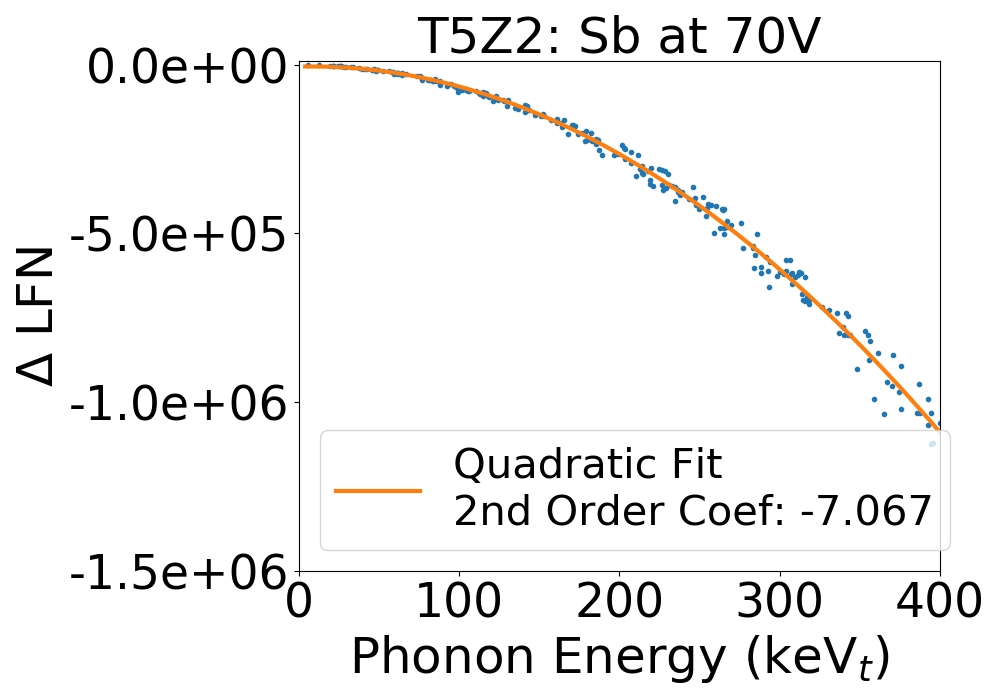
\includegraphics[width=\linewidth]{Figures/QuadraticFit_sbbe_week1_Sample0_Thesis.png}
%  \subcaption{}
\end{minipage}%
\begin{minipage}{.7\textwidth}
  \centering
  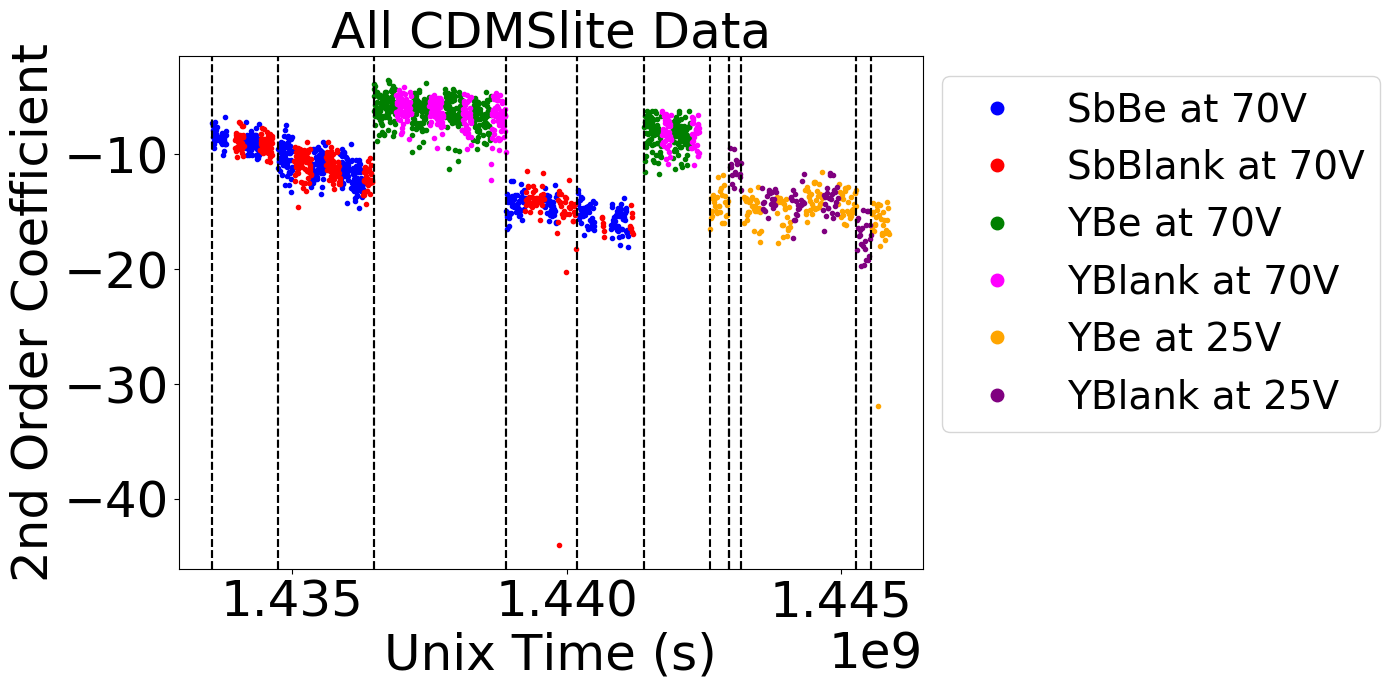
\includegraphics[width=\linewidth]{Figures/dGlitchParabolaCoefVsEventTime_blocks_Thesis.png}
%  \subcaption{figure}
\end{minipage}
}
\caption[Sample plots showing the time block development for the parabolic $\Delta$Glitch and $\Delta$LFN cuts]{Sample plots showing the time block development for the parabolic $\Delta$Glitch and $\Delta$LFN cuts. Left: Quadratic least-squares fit to the $\Delta$LFN distribution for a sample series. Right: Time variation of second-order $\Delta$Glitch parabola coefficients, showing the locations of time blocks based on periods in which the bulk population in the second-order parabolic coefficient remains reasonably constant. The colours of the data points represent the condition in which the data was taken -- for example, the ``SbBe at 70V" shown in blue was taken at a 70V voltage bias, with $^{124}$Sb source and $^9$Be wafer in place.}
\end{figure}

It is worth noting in Fig. 4.11 right that the second-order parabola coefficient gradually decreases within each time block. This pattern appears to arise from a correlation between the second-order parabolic coefficients and the event rate in the detector as the source decays. The correlation is illustrated in Fig. 4.12, and discussed in the figure caption.

\begin{figure}[H]
\centering
\makebox[\textwidth][c]{
\begin{minipage}{.6\textwidth}
  \centering
  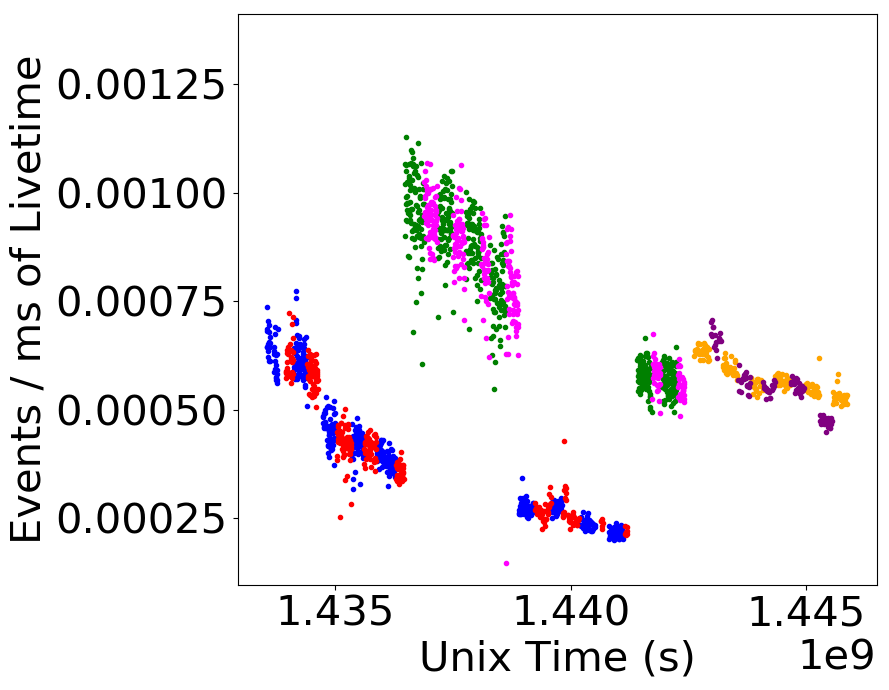
\includegraphics[width=0.95\linewidth]{Figures/EventRateVsEventTime_Thesis.png}
%  \subcaption{}
\end{minipage}%
\begin{minipage}{.6\textwidth}
  \centering
  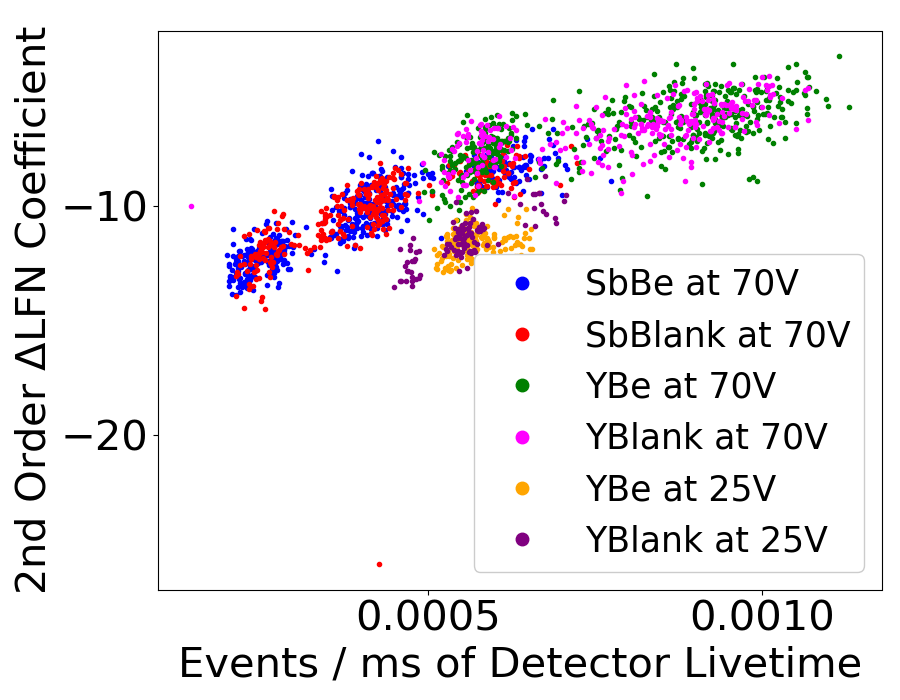
\includegraphics[width=0.95\linewidth]{Figures/ParabolaVsEventRate_Thesis.png}
%  \subcaption{figure}
\end{minipage}
}
\caption[Plots showing the correlation between the event rate in the detector and the second-order $\Delta$LFN parabolic fit coefficient]{Plots showing the correlation between the event rate in the detector and the second-order $\Delta$LFN parabolic fit coefficient. Left: The time variation in event rate as a function of event time shows some clear correlations when compared with the variation in 2nd-order parabola coefficients shown in 4.12 right. Right: The correlation is seen more directly by plotting the variation in the second-order parabola coefficient with event rate. The slight shift in behaviour of the 25V data compared with the 70V data could be due at least in part to the fact that the 25V data was taken with a different detector (T2Z1 rather than T5Z2), and at a different operating voltage.}
\end{figure}

A possible explanation for the observed correlation between the event rate and the second-order parabolic coefficient is as follows: if the event rate is high enough to produce pulses in a significant number of the randoms used to evaluate the noise environment, the calculated noise level would be positively correlated with the event rate. Since the $\chi^2$ decreases as the expected data variation increases, the sizes of the calculated $\chi^2$ quantities should in general be negatively correlated with the calculated noise level. As such, the overall amplitude of the $\chi^2$ values, and linear combinations thereof -- and hence the amplitude of the second-order fit coefficient -- would be negatively correlated with the event rate. This correlation was not investigated further, however, as it was not considered directly relevant for the analysis.

\subsubsection{BadSeries Cut}

The BadSeries cut removes three series that were deemed during the course of the analysis to be unusable due to their exceptionally low noise environment, as measured using the randoms discussed earlier. In principle, an unusually low measured noise environment does not necessarily imply that the data itself is problematic - in fact, raw event traces sampled from these three series appeared quite normal. 

The issue arises from the fact that the measured noise environment affects the calculation of the phonon $\chi^2$ quantities, discussed above in relation to the phonon pulse shape cuts, such that series with a highly atypical measured noise environment tend not to follow the main distribution of events in the phonon $\chi^2$, $\Delta$Glitch, and $\Delta$LFN planes, as shown for one of the series in Fig. 4.13.

\begin{figure}[H]
\centering
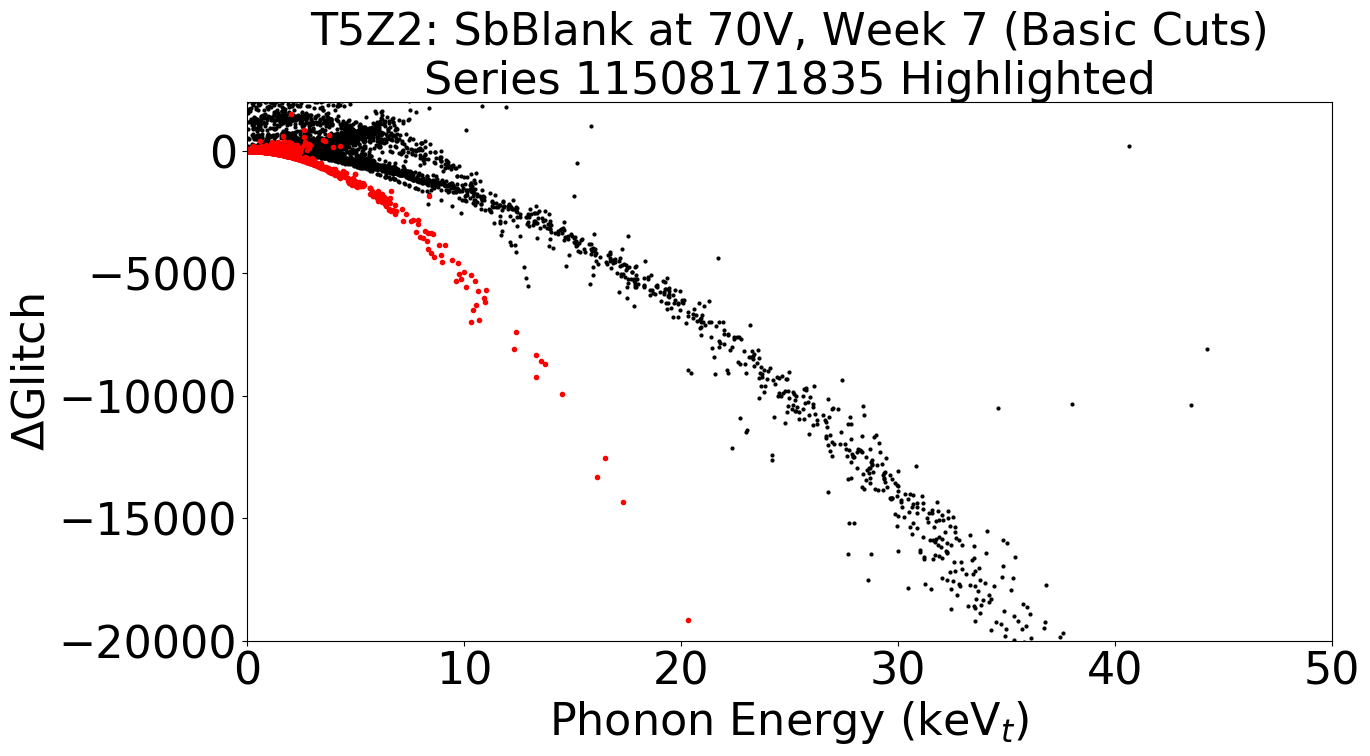
\includegraphics[width=0.8\linewidth]{Figures/dGlitch_down25_Block4_Series11508171835_Thesis.png}
\caption[Sample series removed by the BadSeries cut, showing its energy variation with respect to the $\Delta$Glitch phonon pulse shape variable]{Sample series removed by the BadSeries cut, showing its energy variation with respect to the $\Delta$Glitch phonon pulse shape variable. The series stands out in this plane, such that a $\Delta$Glitch cut that is well tuned for the main distribution of events would be poorly tuned for this particular series.}
\end{figure}


The unusual distribution of these series in the phonon $\chi^2$ planes has two negative effects:

\begin{enumerate}
\item It was found that the RMS and CDF points discussed in Table 4.1 are shifted by these series to the extent that the phonon pulse shape cut definitions would become significantly skewed if the series were not removed.
\item The phonon pulse shape cut definitions developed based on the main distribution of events in each time block would not target these series in the desired manner.
\end{enumerate}

\subsubsection{Charge $\chi^2$ Cut}

The charge $\chi^2$ cut is a flat cut on the $\chi^2$ quantity computed when fitting the summed charge pulse to the ``good charge pulse" template. The $\chi^2$ is summed over both the inner and outer charge channels. The cut was developed for each of the three CDMSlite data sets -- Sb at 70V, Y at 70V, and Y at 25V -- with the aim of removing potential events arising due to electronic glitches in the detector rather than true recoil events that may have been missed by the phonon pulse shape cuts.

\textit{Y at 25V}

The Y at 25V data set, taken with the T2Z1 detector, is plotted in charge $\chi^2$ vs. charge energy space in Fig. 4.14 left. The distribution shows a clear main population of events at relatively low charge $\chi^2$, with a sparse distribution of low-energy events going up to high charge $\chi^2$. 

\begin{figure}[H]
\centering
\begin{minipage}{.5\textwidth}
  \centering
  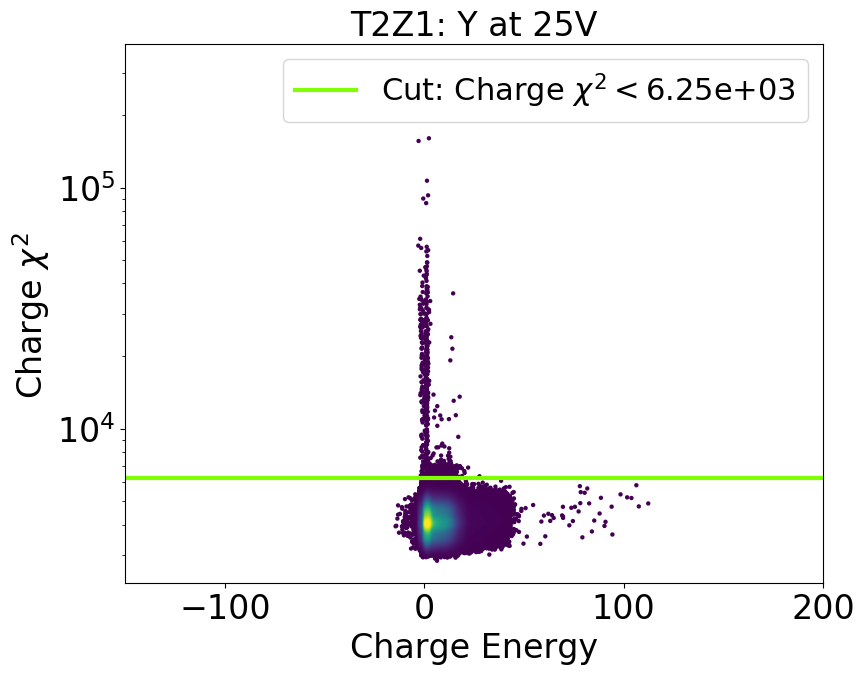
\includegraphics[width=\linewidth]{Figures/ChargeChisq_y_25V_Thesis.png}
%  \subcaption{}
\end{minipage}%
\begin{minipage}{.5\textwidth}
  \centering
  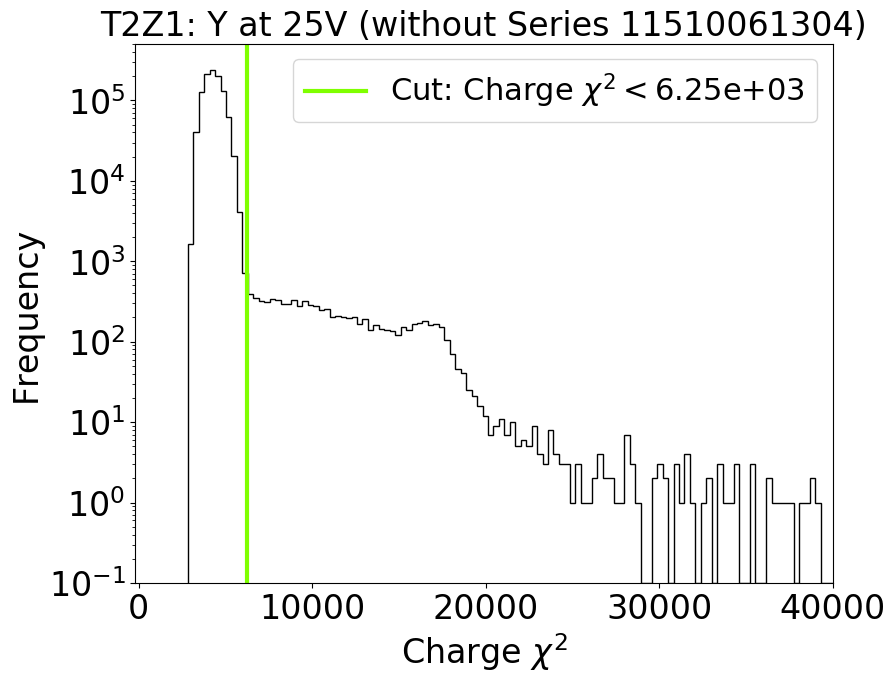
\includegraphics[width=\linewidth]{Figures/ChisqHist_y_25V_nonrandoms_cut_no11510061304_Thesis.png}
%  \subcaption{figure}
\end{minipage}
\caption[Y at 25V data passing the basic and above-discussed quality cuts, showing the location of the charge $\chi^2$ cut]{Y at 25V data passing the basic and above-discussed quality cuts, showing the location of the charge $\chi^2$ cut. Left: Shown in charge $\chi^2$ vs. charge energy space. Right: Charge $\chi^2$ distribution. The exact cut placement is chosen to be near the shoulder of this distribution.}
\end{figure}

The nominal cut in charge $\chi^2$ space was placed based on two considerations:

\begin{enumerate}
\item in what range of charge $\chi^2$ do raw sample charge traces begin to appear visually glitchy, like the charge trace in Fig. 4.15 right, and 
\item at what point does the charge $\chi^2$ distribution exhibit a clear shoulder.
\end{enumerate}

\begin{figure}[H]
\centering
\begin{minipage}{.5\textwidth}
  \centering
  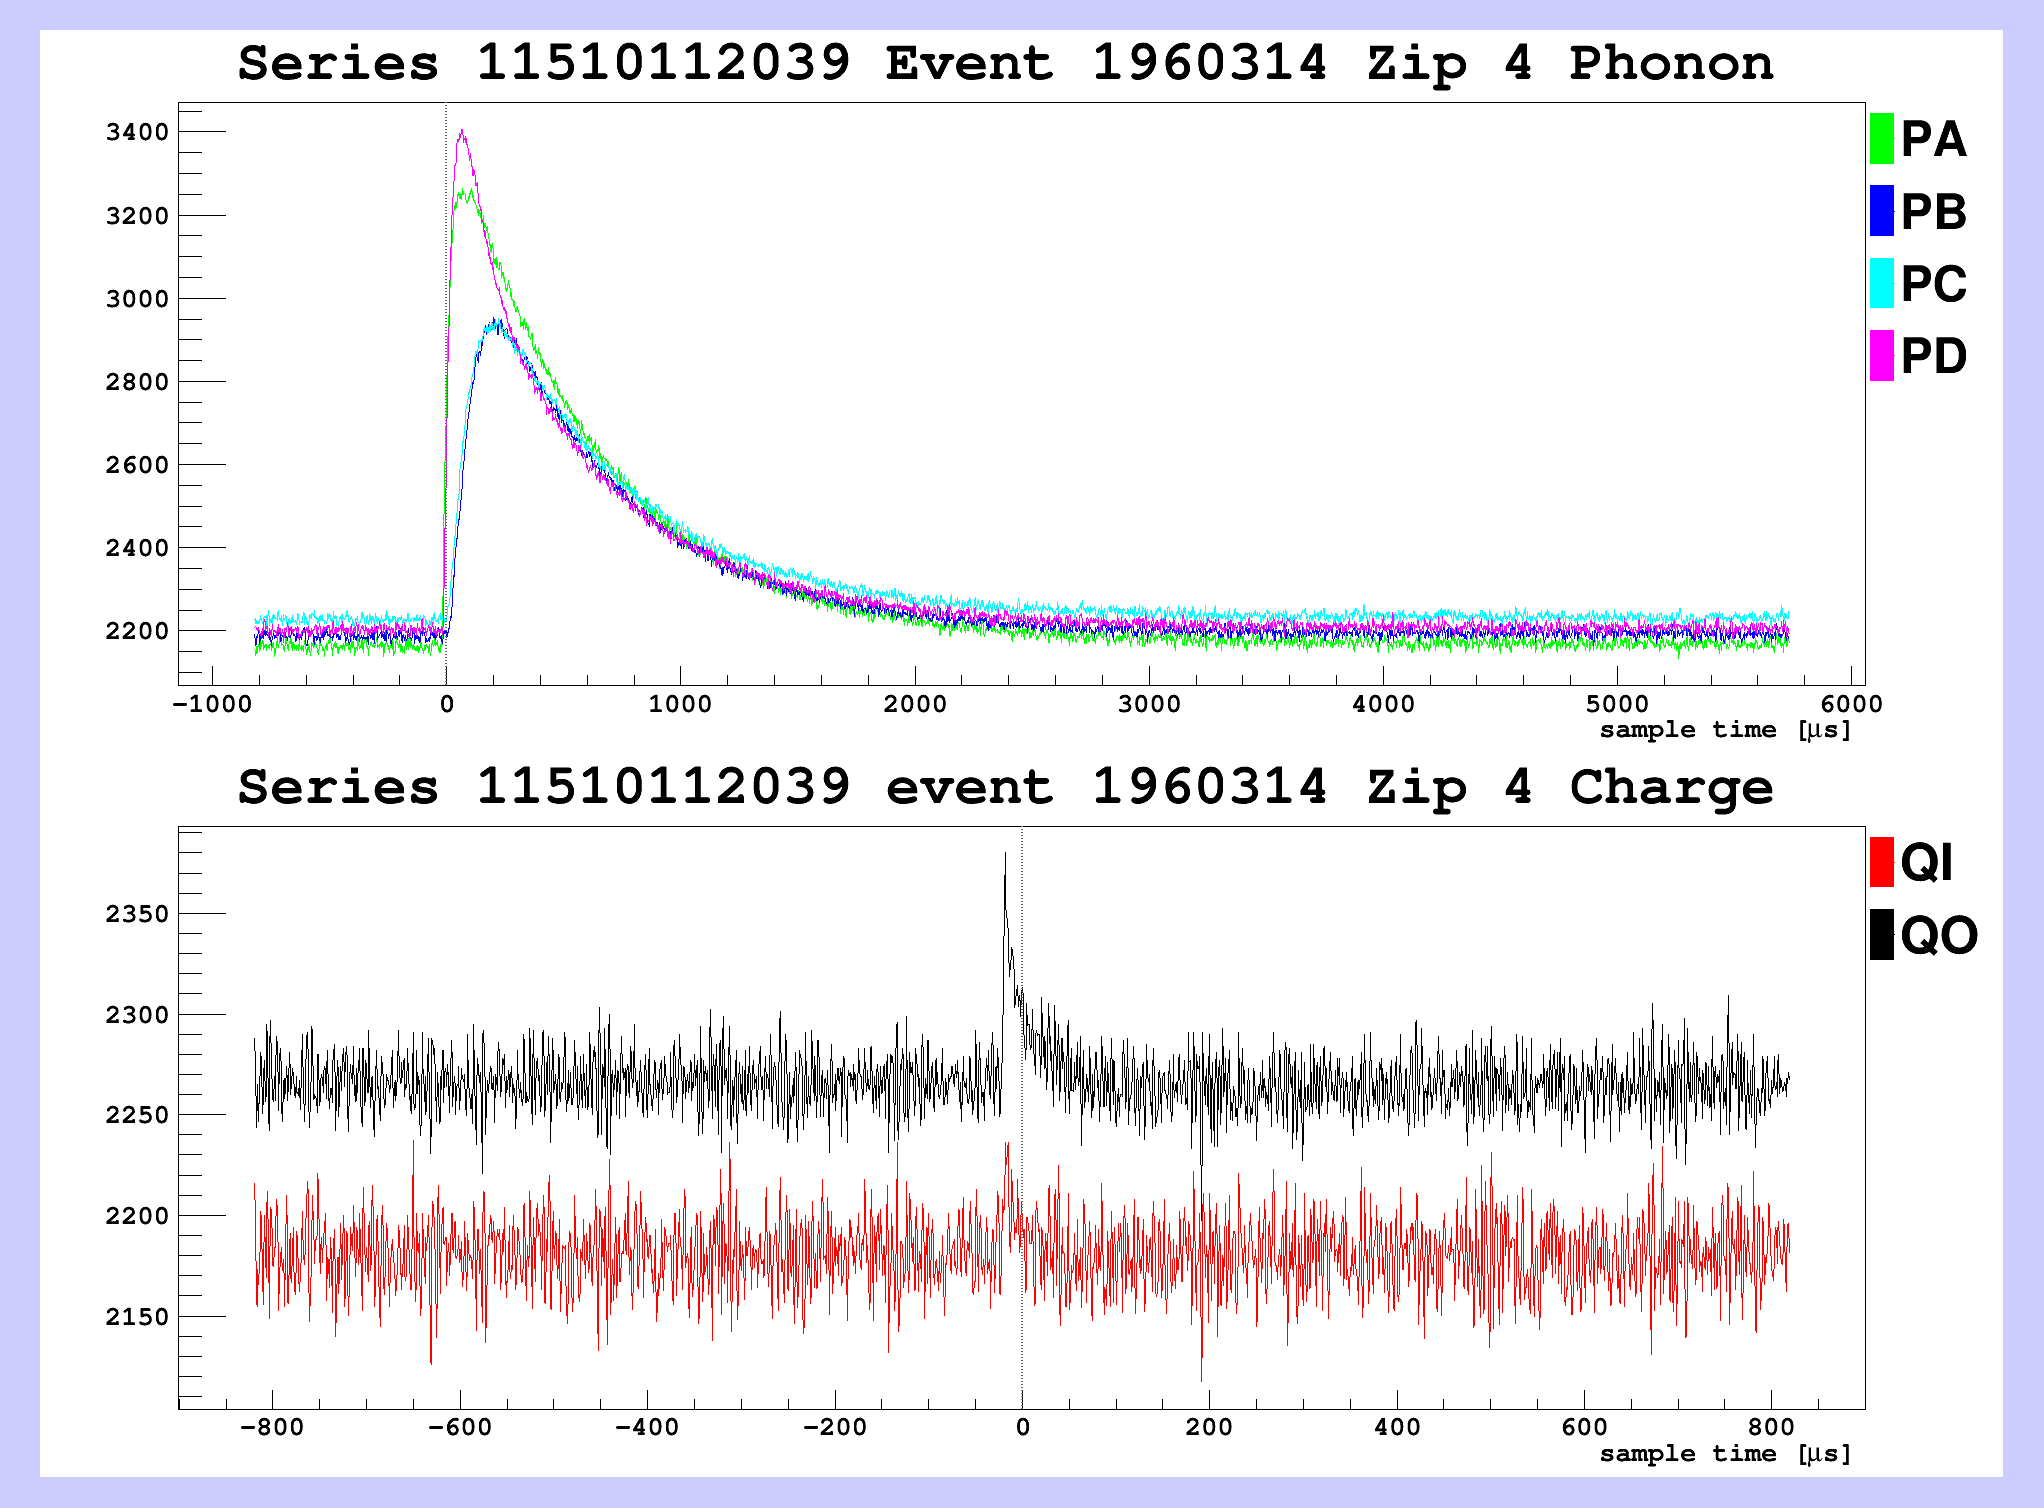
\includegraphics[width=0.95\linewidth]{Figures/RawPulse_GoodCharge.png}
%  \subcaption{}
\end{minipage}%
\begin{minipage}{.5\textwidth}
  \centering
  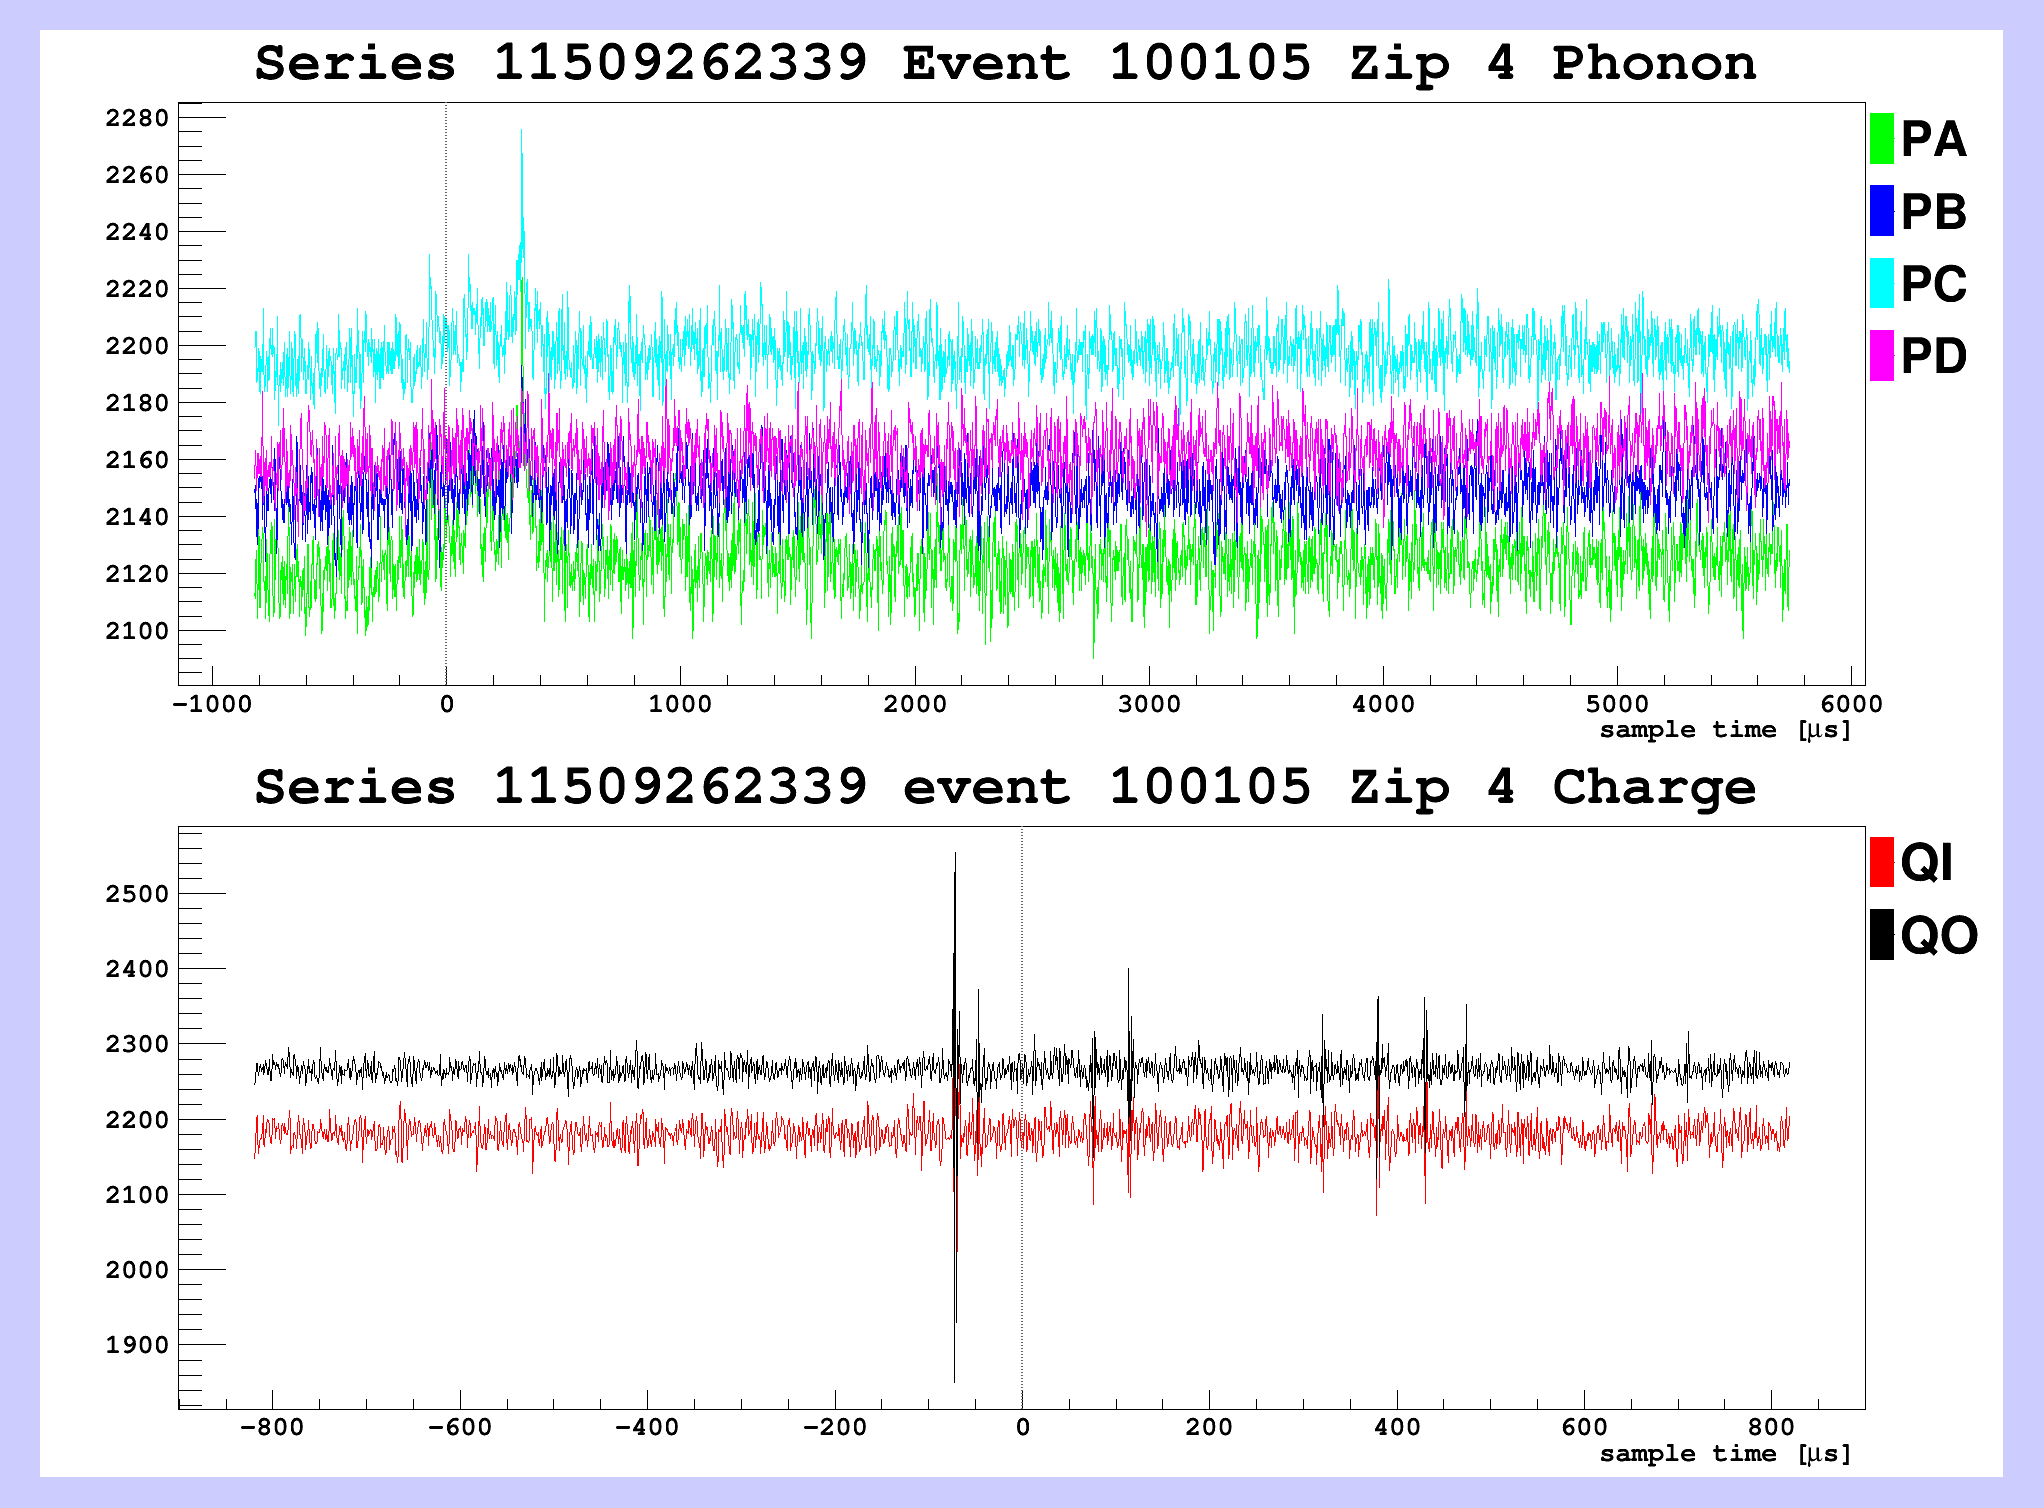
\includegraphics[width=0.95\linewidth]{Figures/RawPulse_BadCharge.png}
%  \subcaption{figure}
\end{minipage}
\caption[Sample raw pulse traces for the charge $\chi^2$ cut]{Sample raw pulse traces for the charge $\chi^2$ cut. The top panel in each plot shows the raw phonon trace, and the bottom panel shows the raw charge trace. Left: ``good" charge trace, without any glitchy behaviour. Right: ``bad" charge trace, with clear glitchy behaviour.}
\end{figure}

Visual inspection of the raw traces revealed that glitchy behaviour like that shown in Fig. 4.15 right began in the range of $6000 <\text{charge }\chi^2 < 7000$. 

Based on the above considerations, the cut for the Y at 25V data is nominally defined as:

\begin{equation}
\nonumber
\text{Charge }\chi^2 < 6250 
\end{equation}

However, there is a conspicuous population of data points, highlighted in red in Fig. 4.16, that appears shifted upward compared with the main distribution. It was found that this population originates from a single series in the neutron-on Y at 25V data.  

\begin{figure}[H]
\centering
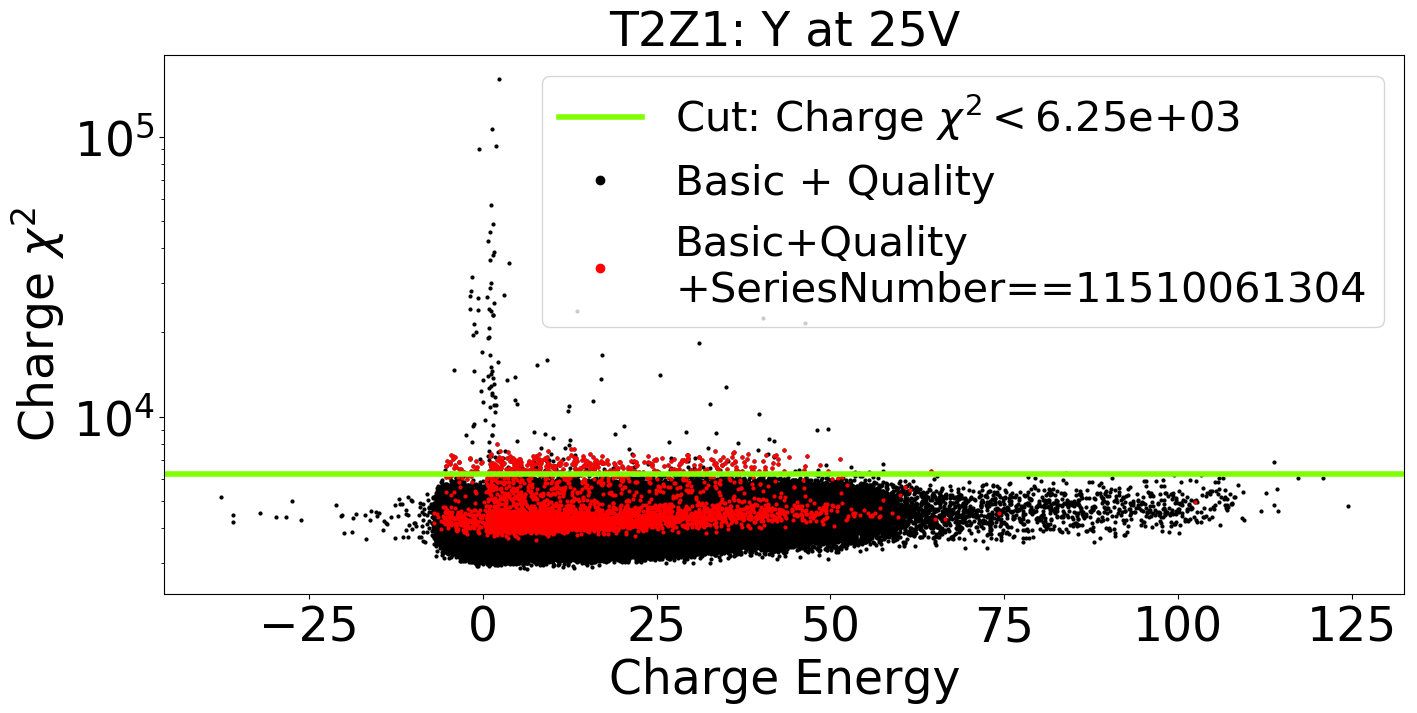
\includegraphics[width=0.8\linewidth]{Figures/YBlank_ChargeChisqVsChargeEnergy_11510061304_Thesis.png}
\caption[Y at 25V: neutron-on data with outlying charge $\chi^2$ highlighted]{Y at 25V: neutron-on data with outlying charge $\chi^2$ highlighted in red. A non-negligible number of events without charge pulse glitches would be removed from this series if the nominal cut were applied to it.}
\end{figure}

An inspection of the raw charge traces from this series revealed that none of the traces for events in this series with charge $\chi^2$ above the nominal cut location appear glitchy, so this particular series was exempted from the charge $\chi^2$ cut to avoid unnecessary removal of data. It is assumed that the shift in charge $\chi^2$ arises from a change in the measured noise environment during that series that affected the $\chi^2$ calculation during processing. Therefore, the final cut definition for the Y at 25V data is:

\begin{equation}
\nonumber
\text{Charge }\chi^2 < 6250\text{, or SeriesNumber==11510061304}
\end{equation}

\textit{Sb at 70V and Y at 70V}

The charge-channel behaviour is quite different in the 70V data sets, which were taken with the T5Z2 detector. In this detector, it is found for many events that the outer (QO) charge channel exhibits sparse, narrow, and isolated glitches, an example of which is shown in Fig. 4.17 left.

\begin{figure}[H]
\centering
\begin{minipage}{.5\textwidth}
  \centering
  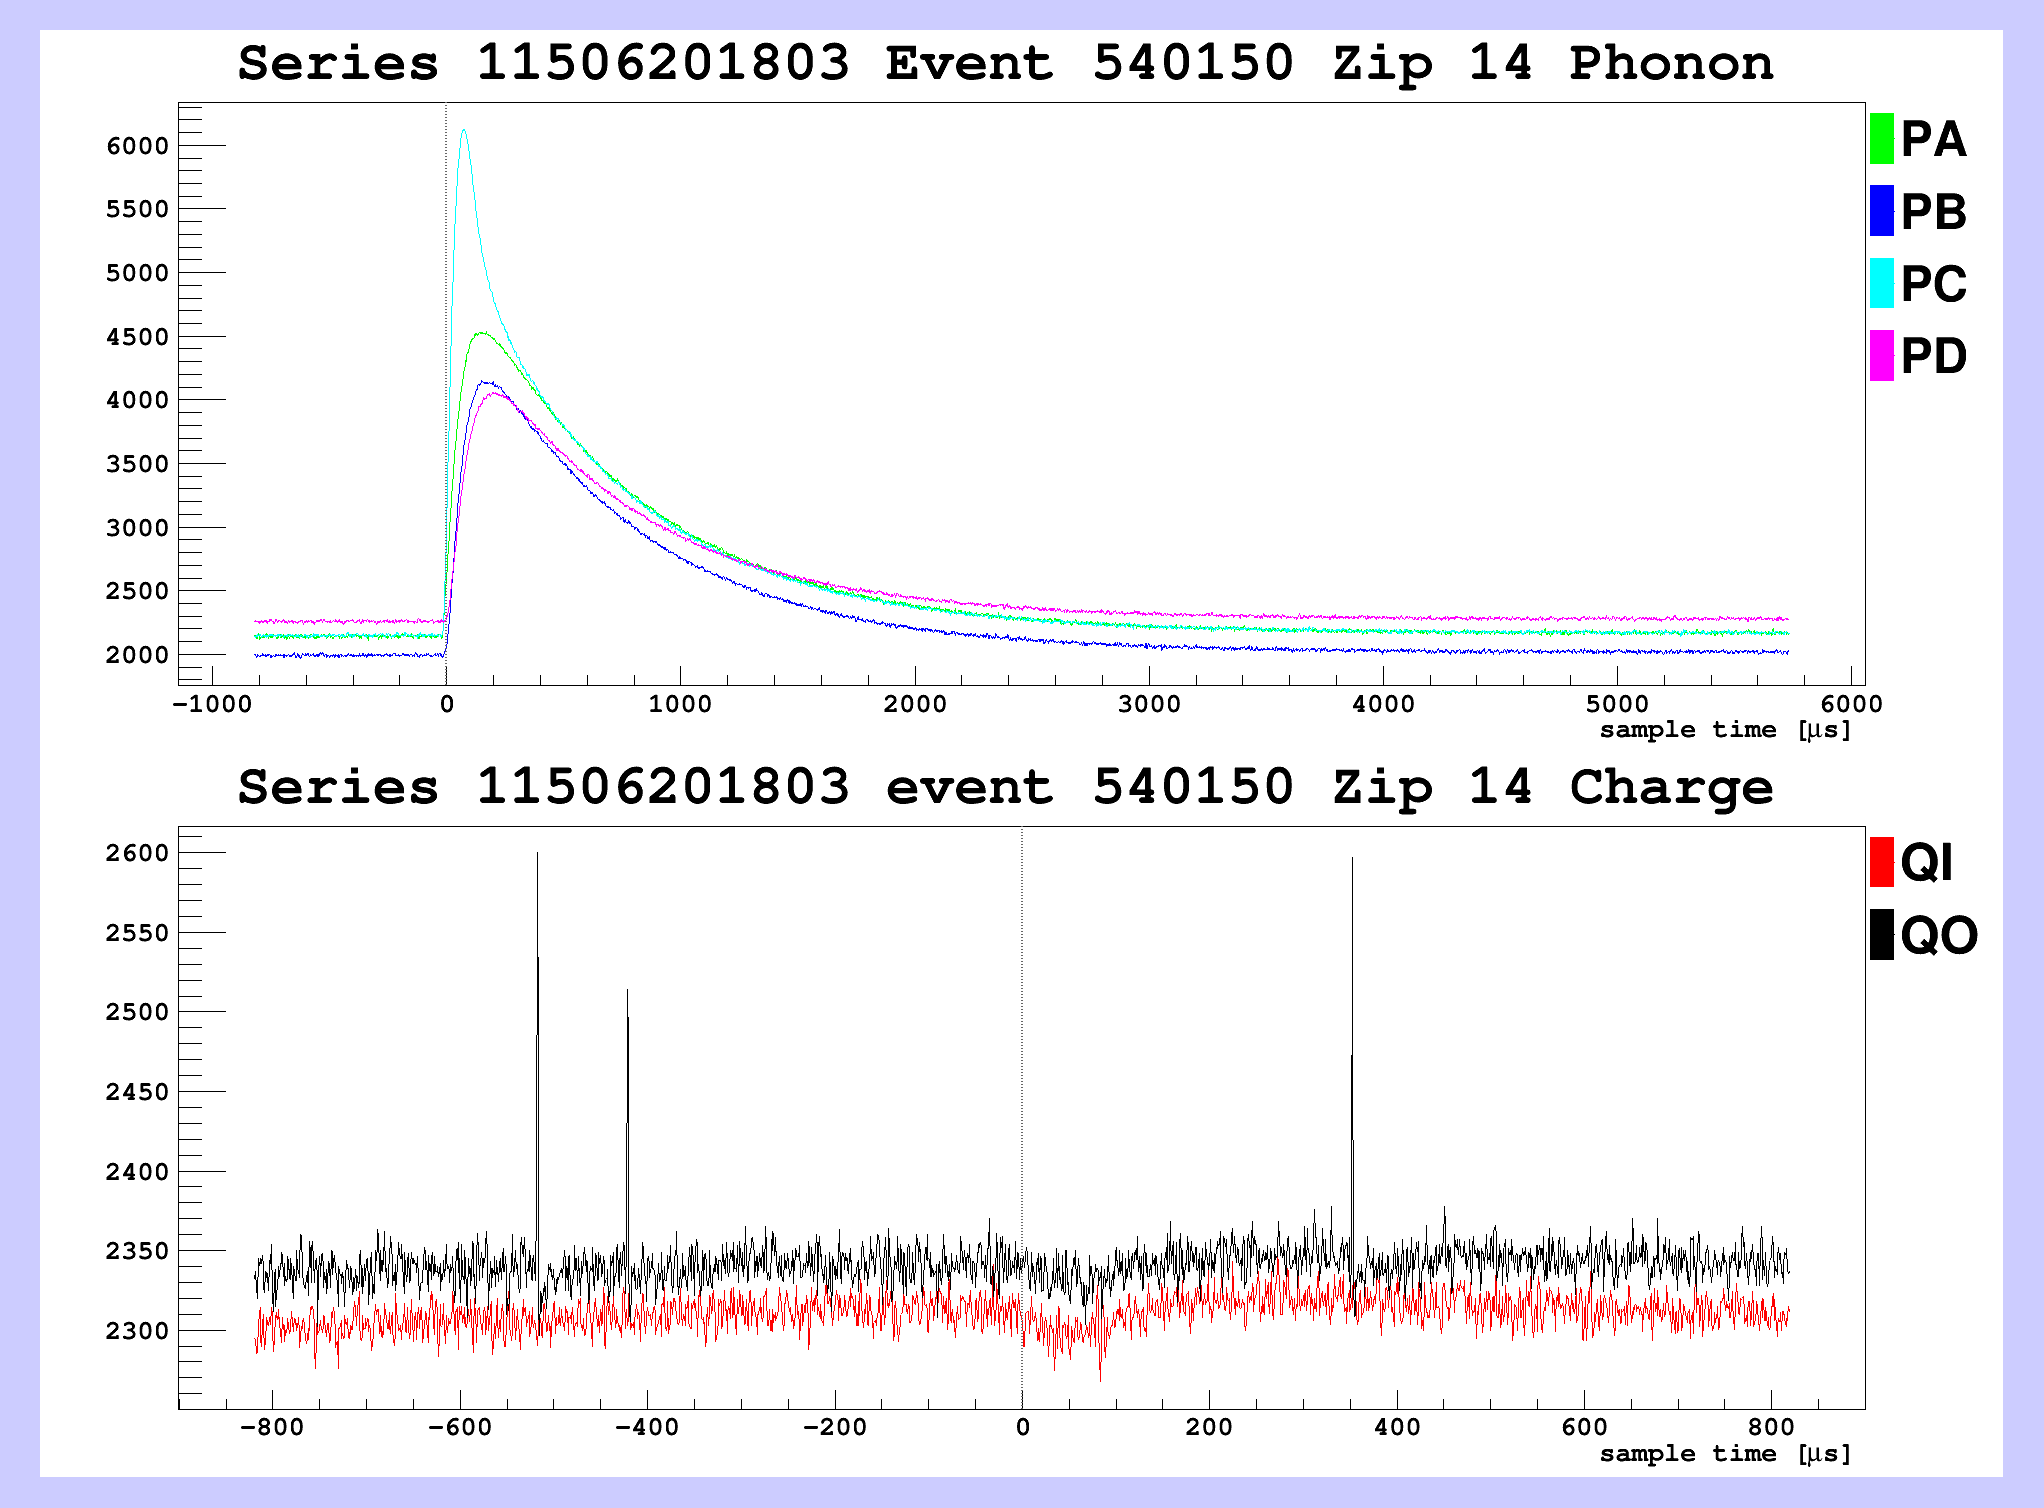
\includegraphics[width=0.95\linewidth]{Figures/SampleIsolatedGlitch.png}
%  \subcaption{}
\end{minipage}%
\begin{minipage}{.5\textwidth}
  \centering
  \includegraphics[width=0.95\linewidth]{Figures/SampleIsolatedAndElectronicGlitches.png}
%  \subcaption{figure}
\end{minipage}
\caption[Two examples of glitchy pulse traces in the 70V data with narrow, isolated glitches]{Two examples of glitchy pulse traces in the 70V data. Left: These glitches are narrow, isolated, and confined to the QO channel. The QI and phonon pulse traces appear reasonable. Right: This trace has a combination of isolated glitches in the QO channel, and electronic glitches such as those seen in Fig. 4.15 right. The electronic glitches are correlated between the QO and QI channels, and the phonon channel does not appear to have a significant pulse.}
\end{figure}

These isolated glitches are suspected to be unrelated to true electronic glitches in the detector, arising instead from issues associated with the outer charge channel readout on T5Z2. This suspicion arises mainly from the following observations:

\begin{enumerate}
\item The isolated QO channel glitches do not correspond to glitches in the inner charge channel (QI) pulse trace, whereas such a correspondence between QI and QO glitches is typically seen for electronic glitches such as that shown in Fig. 4.15 right. 
\item The presence of the isolated glitches does not tend to be correlated with visually glitchy or irregular behaviour in the phonon channel. This correlation is often seen for the electronic glitches found in the Y at 25V data. 
\end{enumerate}

The isolated glitches in the QO channel present a problem for the cut definition because they tend to smear the total charge $\chi^2$ estimates to relatively high values, as shown in Fig. 4.18 left. This creates a degeneracy in charge $\chi^2$ space between events of concern with true electronic glitches, and events with the isolated QO channel glitches that do not appear to be correlated with glitchy behaviour in either of the QI charge channel or the phonon channels, and are therefore not considered to be indicative of glitchy phonon traces. 

\begin{figure}[H]
\centering
\begin{minipage}{.5\textwidth}
  \centering
  \includegraphics[width=0.95\linewidth]{Figures/ChargeChisq_y_70V_Thesis.png}
%  \subcaption{}
\end{minipage}%
\begin{minipage}{.5\textwidth}
  \centering
  \includegraphics[width=0.95\linewidth]{Figures/ChisqHist_y_70V_nonrandoms_locations_Thesis.png}
%  \subcaption{figure}
\end{minipage}
\caption[Y at 70V data passing the above-discussed quality cuts, showing the location of the charge $\chi^2$ cut for the 70V data]{Y at 70V data passing the above-discussed quality cuts, showing the location of the charge $\chi^2$ cut for the 70V data. Right: Charge $\chi^2$ distribution. Due to the isolated QO glitch events described in the text, the distribution does not exhibit the clear shoulder that is seen for the 25V data in Fig. 4.14.}
\end{figure}

As shown in Fig. 4.18 right, the charge $\chi^2$ distribution for the 70V data does not exhibit a shoulder such as that used to guide the choice of cut location in the Y at 25V data. Instead, the approach for setting the cut location of the 70V data is as follows: since the purpose of the charge $\chi^2$ cut is to remove pulses that do not represent real physics events, but which managed to make it through the phonon pulse shape cuts, one would expect some degree of positive correlation between the charge and phonon $\chi^2$ quantities prior to the application of quality cuts, in the region where the charge $\chi^2$ cut is applicable. To verify this approach, the charge and phonon $\chi^2$ quantities are plotted together for the Y at 25V data in Fig. 4.19 left, with only the basic cuts applied. Indeed, the region of charge $\chi^2$ at which positive correlations become apparent roughly corresponds to the cut location obtained by the independent methods discussed previously. An analogous plot for the Sb at 70V data is shown in Fig. 4.19 right.

\begin{figure}[H]
\centering
\begin{minipage}{.5\textwidth}
  \centering
  \includegraphics[width=0.95\linewidth]{Figures/ChisqVsPTNFchisq_y_25V_Thesis.png}
%  \subcaption{}
\end{minipage}%
\begin{minipage}{.5\textwidth}
  \centering
  \includegraphics[width=0.95\linewidth]{Figures/ChisqVsPTNFchisq_sb_70V_Thesis.png}
%  \subcaption{figure}
\end{minipage}
\caption[Variation of phonon $\chi^2$ with charge $\chi^2$, showing the point at which positive correlations become visible between these two $\chi^2$ quantities]{Variation of phonon $\chi^2$ with charge $\chi^2$, showing the point at which positive correlations become visible between these two $\chi^2$ quantities. Left: Verification that the cut location chosen for the Y at 25V data roughly corresponds to the point at which positive correlations are seen between the charge and phonon $\chi^2$. Right: Cut location for the Sb at 70V data, using the charge $\chi^2$ for which positive correlation becomes visible to guide the choice of cut location.}
\end{figure}

Based on the above criterion, the charge $\chi^2$ cut is placed as follows for the 70V data:

\begin{equation}
\nonumber
\text{Charge }\chi^2 < 50,000
\end{equation}

\subsubsection{Low-Frequency Noise Blob Cut}

Low-frequency noise (LFN) represents a particularly significant background for the analysis at low energies near the trigger threshold, where events are predominantly triggered by LFN and electronic glitches, rather than true recoils in the detector. A sample ``LFN blob" is shown in $\Delta$Glitch space for the neutron-off (``blank") data in Fig. 4.20 left. 

The noise blob is effectively removed by the $\Delta$Glitch cut down to a certain energy, below which the noise blob becomes degenerate with the main distribution of events. 

A study was done to evaluate how much the low-energy analysis cutoff would need to be increased above the trigger threshold in order to be confident that the low-frequency noise events would not affect analysis results at a significant level given the statistical uncertainty associated with the experimental spectra. The study was performed by first identifying a region in the low-energy spectrum above which the shoulder of the LFN blob spectrum is reasonably well fit with a decaying exponential $y(E)$:

\begin{equation}
y(E)=Ae^{-(E-E_{min})/E_{1/2}}+B
\end{equation}

where $E$ is the phonon energy (with the usual subscript p removed for notational convenience) $E_\text{min}$ is minimum energy of the fitting region, $E_{1/2}$ is the decay constant of the exponential, A is the amplitude of the exponential fit, and B represents the approximately constant background of electron recoil events. 

\begin{figure}[H]
\centering
\begin{minipage}{.43\textwidth}
  \centering
  \includegraphics[width=0.95\linewidth]{Figures/LFN_Blob_Glitch.png}
%  \subcaption{}
\end{minipage}%
\begin{minipage}{.57\textwidth}
  \centering
  \includegraphics[width=0.95\linewidth]{Figures/blank_ptNFc_Hist_y_70V_log_Thesis.png}
%  \subcaption{figure}
\end{minipage}
\caption[Sample fit to LFN blob for the neutron-off Y at 70V data]{Sample fit to LFN blob for the neutron-off Y at 70V data. Left: Energy distribution of the $\Delta$Glitch variable, in which the LFN blob is found to be best separated from the main distribution. Right: Phonon energy spectrum, with the shoulder of the LFN blob fit with the decaying exponential defined in Eq. 4.6.}
\end{figure}

%The method of determining the energy at which the number of LFN blob events in the spectrum could affect the analysis result is 

Using the pure exponential (i.e. non-background) portion of $y(E)$, the idea is to find the energy $E_0$ below which these LFN blob events can significantly affect the analysis result. Above $E_0$, the contribution of LFN blob events to the energy spectrum should become negligible compared with the scale of Poisson uncertainty associated with the spectrum of true recoil events. The method is illustrated in Fig. 4.21, and detailed below.

\begin{figure}[H]
\centering
\includegraphics[width=0.6\linewidth]{Figures/YellinCutoff_sb_70V_Thesis.png}
\caption[Illustration of the method for determining the optimized analysis cutoff $(E_0)_\text{opt}$]{Illustration of the method for determining the optimized analysis cutoff $(E_0)_\text{opt}$. Top: For values of $E_0$ above $(E_0)_\text{opt}$, the noise blob model (magenta) integrated from $E_0$ out to $\infty$ (I$_\text{blob}$) becomes negligible compared with the Poisson uncertainty $\sqrt{N_\text{Be}}$ (navy points below $(E_0)_\text{opt}$ and lime green points above) associated with the integrated number of neutron-on events between $E_0$ and $E_0+E_{1/2}$ (beige region). Bottom: The exact point above which I$_\text{blob}$ is considered negligible compared with $\sqrt{N_\text{Be}}$ occurs when the ratio $\frac{I_\text{blob}}{\sqrt{N_\text{Be}}}$ drops below $\frac{1}{3}$.}
\end{figure}

For a given candidate value of $E_0$, the LFN model is integrated from $E_0$ out to $\infty$:

\begin{equation}
I_\text{blob} = \int_{E_0}^\infty Ae^{-(E-E_\text{min})/E_{1/2}}dE
\end{equation}

and the total number of events is compared with the Poisson uncertainty $\sqrt{N_\text{Be}}$ associated with the number $N_\text{Be}$ of neutron-on events in a region $\Delta E$ above the candidate analysis threshold $E_0$, where $\Delta E$ -- nominally set to $E_{1/2}$ -- is intended to represent an energy range over which the noise blob is an important component of the spectrum. 

Therefore, the optimum analysis threshold $(E_0)_\text{opt}$ is set as the highest candidate value for which:

\begin{equation}
\frac{I_\text{blob}}{\sqrt{N_\text{Be}}}<\frac{1}{3}
\end{equation}

The cutoff ratio of $\frac{1}{3}$ was chosen to be conservatively less than 1.

\subsubsection{The GoodSeriesRate and TriggerBurst Cuts}

\textit{GoodSeriesRate Cut}

The GoodSeriesRate and TriggerBurst cuts are intended to target periods of data-taking that exhibit unusually high event rates, since the rate of $\gamma$ events in the photoneutron calibration should in theory decay reasonably smoothly as the source decays. As shown in Fig. 4.22, the GoodSeriesRate cut removes entire series whose average trigger rate is significantly above that of nearby series, as this would suggest that many of the events are instrumental background. The location of the GoodSeriesRate cut is chosen for each data set by fitting the event rate decay with an exponential, and vertically shifting the exponential until the cut visually removes the obvious outliers. 

\begin{figure}[H]
\centering
\includegraphics[width=0.6\linewidth]{Figures/EventRateVsEventTime_Fit_sb_70V_detCDMSlite_Thesis.png}
\caption[Time variation of event rate, averaged over each series, for the Sb at 70V data. The GoodSeriesRate cut shown in yellow removes series whose average event rate is significantly above that of nearby series.]{Time variation of event rate, averaged over each series, for the Sb at 70V data. The GoodSeriesRate cut shown in yellow removes series whose average event rate is significantly above that of nearby series.}
\end{figure}

%There are some periods in which the time variation of the event rate fluctuates from a smooth exponential decay for a significant block of series. This suggests there was some change in detector settings that persisted over many series, which is not what the GoodSeriesRate cut is meant to target. Rather, the cut location was set to remove individual series whose event rate was significantly above that of nearby series.

\textit{TriggerBurst Cut}

The idea of the TriggerBurst cut is similar to that of the GoodSeriesRate, except that it operates within each individual series. The idea is to remove periods within a series during which the rate of events passing the basic cuts is too far above the typical event rate in the series. 

Fig. 4.23 shows an example of a series with a period of unusually high event rate highlighted in purple that is removed by even the most conservative TriggerBurst cut considered. The period at the end accumulates events much more quickly than the remainder of the series, indicating that this is a period with an unusually high trigger rate (i.e. a TriggerBurst period).

\begin{figure}[H]
\centering
\includegraphics[width=0.6\linewidth]{Figures/CumLivetime_Thesis.png}
\caption[Example of a series with a period of high trigger rate removed by the TriggerBurst cut]{Example of a series with a period of high trigger rate removed by the TriggerBurst cut.}
\end{figure}

An iterative approach was developed to remove periods of unusually high event rate within a series, as described below: 

\begin{enumerate}
\item First, the events in the series are binned according to the time at which they were measured by the DAQ (also referred to as their ``unix time") into bins approximately 30 seconds in width. Within each bin, an average rate is calculated as the total number of events in the bin, divided by total livetime of events in the bin passing the other basic and quality cuts. The idea is then to remove bins that represent significant outliers due to their high event rate. 
\item The TriggerBurst cut will iteratively remove the bin with the highest event rate, each time re-calculating the mean over the remaining bins until the mean value $\bar{x}$ stabilizes to within the required precision p, expressed in \% as: 

\begin{equation}
p = 100\%\frac{\bar{x}_i-\bar{x}_{i-1}}{\bar{x}_{i-1}}
\end{equation}

where $\bar{x}_i$ is the mean calculated after removing the i$^\text{th}$ outlying bin. Once the precision drops below the required level at the n$^\text{th}$ iteration, the cut is set at a level that removes outlying bins up to the (n-1)$^\text{th}$ iteration. The cut can then be tuned by varying the required precision level of the mean. Fig. 4.24 shows an example of a series with several bins that would be removed by the TriggerBurst cut, depending on the precision level.

\begin{figure}[H]
\centering
\includegraphics[width=0.8\linewidth]{Figures/EvRate_Hist_sbbe_3_Series1_DetCDMSlite_good_rate_Precision_Thesis.png}
\caption[Sample series showing the application of the TriggerBurst cut at varying precision levels]{Sample series showing the application of the TriggerBurst cut at varying precision levels. The bins removed by each precision level are highlighted with a marker whose colour corresponds to the precision level listed in the legend, and the dashed line of the same colour shows the event rate level above which bins are removed for the given precision requirement. Note that, in some cases, several different precision levels will produce the same cut, in which case the largest precision level that produces the cut is shown.}
\end{figure}

\end{enumerate}

Beyond this basic cut-setting algorithm, there is an additional subtlety arising from the fact that not all series were taken for the same amount of time. With 30s bin widths, this means that not all series have the same number of bins. It can be shown (see Appendix A) that the shift $\Delta\bar{x}$ in the mean $\bar{x}$ due to an outlier varies on average with the number of bins N as:

\begin{equation}
\Delta\bar{x} \propto \frac{1}{N}
\end{equation}

To address this issue, the candidate precision level p$_{100}$ is chosen for series with 100 bins, and the actual required precision levels p$_M$ for a series with M bins is defined as:

\begin{equation}
p_M = \frac{p_{100}M}{100}
\end{equation}

The exact precision level requirement for the TriggerBurst cut is tuned for each data set by producing corresponding Monte Carlo (MC) data sets with the typical 30s bin width and Poisson-distributed event numbers, and applying the TriggerBurst cut to the MC data sets to compare the cut's passage fraction. 

The event rate, and hence the mean number of events per bin, decreases both between and within each data set due to the decay of the sources. In order to make the harshest possible estimate of how low the passage fraction could be for Poisson-distributed events in a given data set, the median number of events per bin was determined for each series in the data set with at least 50 bins. The lowest median from all the series was then used as the mean value of the parent Poisson distribution of events-per-bin when producing the MC histograms for that data set. The results are listed for each data set in Table 4.2.

\begin{table}[H]
\centering
\caption[Lowest median events/bin of all series in each data set, and typical number of 30s bins per series]{Lowest median events/bin of all series in each data set, and typical number of 30s bins per series. Both values were used for producing the MC data sets. Note that the number of bins in the 25V data is triple that of the 70V data because the run lengths for these series were 3h rather than 1h. }
\label{my-label}
\begin{footnotesize}
\renewcommand{\arraystretch}{1.5}
\begin{tabular}{|p{20mm}|L{35mm}|L{40mm}|}
\hline
\textbf{data set} & \textbf{Minimum Events/Bin} & \textbf{Typical Number of Bins Per Series} \\ \hline
Sb at 70V & 9 &  100        \\ \hline
Y at 70V & 28 &  100        \\ \hline
Y at 25V & 20 &  300        \\ \hline
\end{tabular}
\end{footnotesize}
\end{table}

Fig. 4.25 shows a sample MC series for the Sb at 70V data, with several bins removed by the TriggerBurst cut. Table 4.3 shows a comparison of event passage fractions for the cut between the experimental data with basic and other quality cuts pre-applied, and the MC data set. There are two criteria used to select the chosen precision level highlighted in Table 4.3.

\begin{enumerate}
\item The passage fraction for Poisson-distributed MC event number histograms should be very high (above 99\%), thus indicating that the cut is not removing a significant amount of normal Poisson fluctuation.  
\item While achieving a very high MC passage fraction, it is also desirable to maximize the difference between MC passage fraction and the passage fraction of the actual data, as this would suggest that the cut is actually removing periods of high trigger-rate bursts, rather than just normal Poisson fluctuations. 
\end{enumerate}

\begin{figure}[H]
\centering
\includegraphics[width=0.8\linewidth]{Figures/EvNum_Hist_9Num_100Bins_Thesis.png}
\caption[Sample MC series for the Sb at 70V data, with the TriggerBurst cut applied]{Sample MC series for the Sb at 70V data, with the TriggerBurst cut applied as described in the caption of Fig. 4.24.}
\end{figure}

\begin{table}[H]
\centering
\caption[Comparison between actual and simulated event passage fractions for Sb at 70V]{Comparison between actual and simulated event passage fractions for Sb at 70V, with the chosen precision level highlighted in bold font. Note that the precision level listed in the left-most column refers to the nominal precision level p$_{100}$ for a series with 100 bins (see Eq. 4.11 for the conversion to the true precision level for a given series).}
\label{my-label}
\begin{footnotesize}
\renewcommand{\arraystretch}{1.5}
\begin{tabular}{|p{30mm}|L{25mm}|L{25mm}|L{25mm}|}
\hline
\textbf{TriggerBurst Cuts} & \textbf{Experimental Event Passage Fraction (\%)} & \textbf{Simulated Event Passage Fraction (\%)} & \textbf{Difference in Passage Fractions (\%)} \\ \hline
None &  100.00 &   100.00  &    0.00     \\ \hline
+2.0\% Precision &  99.58  &    99.999 &   +0.42          \\ \hline
+1.75\% Precision &  99.28  &   99.997  &   +0.72      \\ \hline
+1.5\% Precision &  98.71  &   99.976  &   +1.27      \\ \hline
+1.25\% Precision &  98.71  &   99.835  &  +1.13       \\ \hline
\textbf{+1.0\% Precision} &   \textbf{95.79}   &   \textbf{99.044}  &   \textbf{+3.25}      \\ \hline
+0.85\% Precision &  93.62  &   97.361  &   +3.74      \\ \hline
\end{tabular}
\end{footnotesize}
\end{table}

The precision levels for the Y at 70V and Y at 25V data were set by an analogous procedure to 0.85\% and 1.0\%, respectively.

%\begin{enumerate}
%\item Some series contain bins with zero events, which pull down the mean. 4.26 shows a particularly bad case in which there is a long period of zero-rate bins. In this extreme example, all the bins with non-zero event rate would be removed by the TriggerBurst cut at most precision levels considered. To deal with this, any bins with zero event rate are excluded when computing the mean event rate. 
%
%\begin{figure}[H]
%\centering
%\begin{minipage}{.5\textwidth}
%  \centering
%  \includegraphics[width=0.95\linewidth]{Figures/EvRate_Hist_sbbe_5_Series1_DetCDMSlite_good_rate_Precision_Thesis_noZeroRate.png}
%%  \subcaption{}
%\end{minipage}%
%\begin{minipage}{.5\textwidth}
%  \centering
%  \includegraphics[width=0.95\linewidth]{Figures/EvRate_Hist_sbbe_5_Series1_DetCDMSlite_good_rate_Precision_Thesis.png}
%%  \subcaption{figure}
%\end{minipage}
%\caption[Example series showing the importance of zero-rate bins for the TriggerBurst cut]{zzz}
%\end{figure}
%\end{enumerate}


\subsubsection{TriggerGlitch Cut}

The TriggerGlitch cut is applied in addition to the $\Delta$Glitch cut as a means of identifying and removing pulses produced by electronic glitches. When an event is triggered, the DAQ system records which detectors triggered in both the charge and phonon channels within 1ms of the global trigger time. This information is combined during processing to produce the ``ntrigp/q"quantities, defined as the total number of running detector sides -- of which there are 12 for the photoneutron analysis -- that produced a phonon (ntrigp) or charge (ntrigq) trigger. The $\Delta$ntrig quantity is then constructed as the difference between the number of phonon and charge triggers:

\begin{equation}
\Delta \text{ntrig} = \text{ntrigp}-\text{ntrigq}
\end{equation}

Since a pulse produced by a recoil event should ideally produce triggers in both the charge and phonon channels, the idea of the cut is to remove events for which too many detectors produced a phonon trigger without an accompanying charge trigger.

As shown in Fig. 4.26 top, events with relatively high values of $\Delta$ntrig stand out in several parameters, most notably the x and y partition parameters, which are calculated using the relative pulse amplitudes in the three inner phonon channels to give a coarse estimate of the location of the event in the detector.

\begin{figure}[H]
\centering
\begin{minipage}{.8\textwidth}
  \centering
  \includegraphics[width=0.9\linewidth]{Figures/xyPartitionVsptNF_density_DetCDMSlite_sb_70V_Quality_TrigGlitch_Thesis.png}
%  \subcaption{}
\end{minipage}%

\begin{minipage}{.75\textwidth}
  \centering
  \includegraphics[width=0.9\linewidth]{Figures/SquarePulse.png}
%  \subcaption{figure}
\end{minipage}
\caption[Plots illustrating the effect of the TriggerGlitch cut]{Top: The red population of events in the upper right corner of the x vs. y partition with high $\Delta$ntrig do not follow the main distribution, but are partially degenerate with it. This population is fully removed by the TriggerGlitch cut. Bottom: Events with high $\Delta$ntrig often exhibit these sharp, square phonon traces in all detectors, which from visual inspection are clearly not good signal events.}
\end{figure}

Examining raw pulse traces, it is found that events with $\Delta$ntrig$\geq4$ can produce short, square-shaped pulses such as the one shown in Fig. 4.26 bottom that are visually identified as instrumental artifacts, but which pass the existing basic and quality cuts. These events are removed with the following TriggerGlitch cut:

\begin{equation}
\Delta \text{ntrig} < 4
\end{equation}

\section{Energy Resolution Model}

The total energy resolution $\sigma_T$ of SuperCDMS detectors varies with recoil energy, and is generally modelled by the quadrature sum of three contributions:

\begin{equation}
\sigma_T(E_{ee}) = \sqrt{\sigma_0^2 + F\epsilon E_{ee} + (AE_{ee})^2}
\end{equation}

where:
\begin{itemize}
\item $E_{ee}$ is the energy of the recoil event, assuming an electron recoil, with energy measured in ``keV$_{ee}$".
\item $\sigma_0$ is the baseline resolution at $E_{ee}=0$ due to the detector electronics. 
\item F is the ``Fano factor" that gives a measure of the variance in the number $N_{e/h}$ of e-h pairs ionized by a single recoil. For sufficiently high statistics, the rms statistical fluctuation in N is given by \cite{LukePhonon} $\sqrt{FN_{e/h}}$.
\item $AE_{ee}$ is an empirical term that models any detector effects such as position dependence. 
\end{itemize}

In order to fit this model to the photoneutron data for each of the two CDMSlite detectors, it is necessary to have measurements of the energy resolution at as many recoil energies as possible. These are obtained using ``post-Cf" low-background WIMP search data that was collected shortly after a $^{252}$Cf neutron activation of the detectors. 

During neutron activation, neutrons are captured by $^{70}$Ge nuclei in the detector to form $^{71}$Ge, which is unstable, and decays via electron capture of inner K, L, or M shell electrons to $^{71}$Ga with a half-life of 11 days. Following an electron capture, an outer electron drops down to fill the inner electron shell vacancy, producing one or more characteristic X rays with energies of 10.37 keV$_{ee}$, 1.30 keV$_{ee}$, and 0.16 keV$_{ee}$, which respectively correspond to K, L, and M shell vacancies. The post-$^{252}$Cf data therefore has spectral peaks at these three characteristic X ray energies, and the measured widths of these peaks represent the detector energy resolution at these energies.

The original phonon energy scale (keV$_t$) is converted to keV$_{ee}$ by fitting Gaussian distributions to the L and K shell spectral peaks using a simple least-squares fitting routine, and comparing the centroids of the fitted Gaussian distributions to the known peak energies to obtain a conversion factor. The Gaussian distributions $g(E_{ee})$ are given by:

\begin{equation}
g(E_{ee}) = Ae^{-\frac{(E_{ee}-(E_{ee})_0)^2}{2\sigma^2}}+B
\end{equation}

where A, B, and $(E_{ee})_0$ are fit parameters.

The baseline resolution $\sigma_0$ is measured using the reconstructed energies of random traces from the low-background data, which should be 0 since they do not in general contain pulses. The peak in the energy spectrum of the randoms is fit with a Gaussian distribution, as shown for T2Z1 at 25V in Fig. 4.27, and $\sigma_0$ is taken to be the standard deviation of the fitted Gaussian distribution. 

\begin{figure}[H]
\centering
\includegraphics[width=0.7\linewidth]{Figures/ptNFcee_EORRandom_Bg_25V_Thesis.png}
\caption[Gaussian fit to the zero-energy peak of the randoms to obtain the baseline energy]{Gaussian fit to the zero-energy peak of the randoms to obtain the baseline energy}
\end{figure}

The resolutions at the L, K, and M shell $\gamma$ peaks are also fit with Gaussian distributions to obtain the energy resolution at each shell energy. In the case of the 70V M shell peak, it was not possible to fit a Gaussian distribution due to limited statistics. 

%\begin{figure}[H]
%\centering
%\includegraphics[width=0.7\linewidth]{Figures/Lshell_Bg_25V.png}
%\caption[Gaussian fit to the zero-energy peak of the randoms to obtain the baseline energy ]{zzz}
%\end{figure}

\subsection{Fit to the Resolution Model}

The resolutions obtained at the baseline, M shell, L shell, and K shell are fit with the energy resolution model to obtain the model parameters. The baseline resolution $\sigma_0$ is fixed to the value obtained from the standard deviation of the Gaussian fit described in Section 4.5.1 to reduce the number of degrees of freedom, given the limited number of data points available. The fits to the resolution model are shown for both detectors (T5Z2 and T2Z1) in Fig. 4.28. 

\begin{figure}[H]
\centering
\begin{minipage}{.5\textwidth}
  \centering
  \includegraphics[width=0.95\linewidth]{Figures/ResolutionModel_EORRandom_70V_baseline_Thesis.png}
%  \subcaption{}
\end{minipage}%
\begin{minipage}{.5\textwidth}
  \centering
  \includegraphics[width=0.95\linewidth]{Figures/ResolutionModel_EORRandom_25V_baseline_Thesis.png}
%  \subcaption{figure}
\end{minipage}
\caption[Fits to the detector resolution model using standard deviations of Gaussian fits to spectral peaks]{Fits to the detector resolution model using standard deviations of Gaussian fits to spectral peaks. Left: T5Z2 biased at 70V. Right: T2Z1 biased at 25V.}
\end{figure}

The fit is done using the orthogonal distance regression (ODR) method \cite{ODR}. The major benefit of the ODR method in this instance is that the fit can be weighted by the data covariance matrices in both the x and y coordinates. Since the uncertainty in the energy is non-negligible in this case -- especially for the T2Z1 data shown on the right side of Fig. 4.28 -- it is desirable to account for it in the fit.

The error band $\Delta \sigma_T(E_{ee})$ is calculated as follows using the parameter covariance matrix returned by the fit:

\begin{small}
\begin{equation}
    \Delta \sigma_T(E_{ee}) = \sqrt{\Bigg(\frac{\partial \sigma_T}{\partial A}\Bigg)^2 \text{var}(A) + \Bigg(\frac{\partial \sigma_T}{\partial (F\epsilon)}\Bigg)^2 \text{var}(F\epsilon) + 2\Bigg(\frac{\partial \sigma_T}{\partial A}\Bigg)\Bigg(\frac{\partial \sigma_T}{\partial (F\epsilon)}\Bigg)\text{cov}(A, F\epsilon) }
\end{equation}
\end{small}

where

\begin{equation}
\frac{\partial \sigma_T}{\partial A} = \frac{AE_{ee}}{\sigma_T} \quad\text{, }\quad \frac{\partial \sigma_T}{\partial (F\epsilon)} = \frac{E_{ee}}{2\sigma_T}
\end{equation}

\section{Background Modelling}

The negative log likelihood fit to the Lindhard model, discussed in Section 4.7, is unbinned to avoid any bias associated with the choice of binning. It is therefore not possible to directly subtract the neutron-off $\gamma$ background and fit to the resulting experimental neutron spectrum, since doing so would require binning the data. Instead, a background model is developed which can be incorporated into the probability density function (PDF) used for the likelihood fit. 

The neutron-off $\gamma$ background model is comprised of four components, which are listed below.

\textbf{1. Compton Steps}

The low-energy steps corresponding to each of the Ge electron shells are predicted to arise in the low-energy $\gamma$ background spectrum due to the minimum energy required to free electrons from each shell. For example, incident $\gamma$ rays with energy below the K shell binding energy of 11.1 keV will only be able to free electrons from the L, M, and N electron shells, and will consequently have a slightly lower probability of depositing energy in the detector than $\gamma$ rays above this binding energy. 

It has previously been shown \cite{Compton_Barker} that these steps can be resolved in SuperCDMS detectors operating in CDMSlite mode. For the CDMSlite data taken at 70V, only the L, K, and M shell Compton steps have energy above the analysis threshold. For the 25V data, the M shell step is expected to occur below the analysis threshold, and so is excluded from the model. 

The steps are modelled by two (25V) or three (70V) error functions -- one at each step -- on top of a flat background. For the 25V data, the Compton model is:


\begin{equation}
f_\text{C,25\text{V}}(E_{ee}) = a_0\{1+ \mathcal{S}_L f_\text{st}(E_{ee}, \mu_L)\} + 
\end{equation}
$$+\mathcal{S}_Ka_0\{1+\mathcal{S}_Lf_\text{st}(E_{ee}, \mu_L)\}f_\text{st}(E_{ee}, \mu_K)$$


where $\mathcal{S}$ is the fractional step amplitude, and $a_0$ is the flat background level. The step sizes and background level are left as fit parameters. $\mu$ is the central energy of the step, which was determined for each step by another member of the collaboration using a Geant4 simulation. $f_\text{st}$ is the error function step:

\begin{equation}
f_\text{st}(E_{ee}, \mu) = \frac{1}{2}\Bigg[1+\text{erf}\Bigg(\frac{E_{ee}-\mu}{\sqrt{2}\cdot \sigma(\mu)}\Bigg)\Bigg]
\end{equation}

$\sigma(\mu)$ is the detector energy resolution at the centroid of the step, and is not fit for, but instead obtained from the resolution model discussed in Section 4.5. 

For the 70V data, the model additionally includes an M shell step:

\begin{equation}
f_\text{C,70\text{V}}(E_{ee}) = a_0\{1+ \mathcal{S}_M f_\text{st}(E_{ee}, \mu_M)\} + 
\end{equation}
$$+\mathcal{S}_La_0\{1+\mathcal{S}_Mf_\text{st}(E_{ee}, \mu_M)\}f_\text{st}(E_{ee}, \mu_L)+$$
$$+\mathcal{S}_Ka_0\Big[\{1+\mathcal{S}_Mf_\text{st}(E_{ee}, \mu_M)\}f_\text{st}(E_{ee}, \mu_L)\Big]f_\text{st}(E_{ee}, \mu_K)$$

\textbf{2. Polynomial Component}

A polynomial component of order 3 is included to model any large-scale variation in addition to the theoretical Compton step background due to energy variation in the both the ``cut efficiencies" and in the fraction of instrumental background events that are removed by the data cuts. The efficiency of a cut is defined as the fraction of true signal events produced by recoils in the detector that are retained after the cut is applied. The polynomial component is given by:

\begin{equation}
f_\text{p}(E_{ee}) = a_1(E_{ee})+a_2(E_{ee})^2+a_3(E_{ee})^3
\end{equation}

\textbf{3. Post-Cf Peaks}

A $^{252}$Cf detector calibration ended nine days before data-taking began for the photoneutron calibration -- less than the 11-day half life of electron captures following neutron activation (see Section 4.5 for further details of the neutron activation). The fractional electron capture probabilities for each shell of $^{71}$Ge were calculated by another member of the collaboration using the method of \cite{EC} to be $B_K=87.57$\%, $B_L=10.53$\%, and $B_M=1.78$\% for the K, L, and M shells, respectively. Using this information, an additional term modelling the post-$^{252}$Cf electron capture peaks is added to the background model:

\begin{equation}
f_\text{Cf}(E_{ee}) = A_K \Bigg\{\text{Gauss}(E_{ee}, E_K, \sigma(E_K)) +
\end{equation}
$$+ \frac{B_L}{B_K}\text{Gauss}(E_{ee}, E_L, \sigma(E_L)) + \frac{B_M}{B_K}\text{Gauss}(E_{ee}, E_M, \sigma(E_M)) \Bigg\}$$

where

\begin{equation}
\text{Gauss}(E_{ee}, E_\text{peak}, \sigma(E_\text{peak})) = e^{-(E_{ee}-E_\text{peak})^2/(2\sigma(E_\text{peak})^2)}
\end{equation}

$A_K$, the amplitude of the K shell peak, is the only fit parameter. $E_K=10.37$ keV$_{ee}$, $E_L=1.30$ keV$_{ee}$, and $E_M=0.16$ keV$_{ee}$ are the energies of each peak, and the peak widths $\sigma(E_\text{peak})$ are obtained from the resolution model discussed in Section 4.5. The M shell peak is excluded from the post-$^{252}$Cf model for the Y at 25V data, because the M shell peak energy, converted to phonon energy using Eq. 3.4 with $Y=1$, is below the analysis threshold for this data set.

\textbf{4. Smoothing Component}

It was found that the background model obtained from the analytical components described above cannot alone yield an acceptably good fit to the experimental data, as indicated by a low p-value based on the calculated fit $\chi^2$ and degrees of freedom, as well as visible structure in the fit residuals. Careful checks were done to rule out the possibility of appreciable contributions to the $\gamma$ background from:

\begin{itemize}
\item primary X-rays or electrons from the radioactive source, or
\item secondary particles produced as decay products following $\gamma$ activation of the Ge crystals or surrounding material by $\gamma$ rays from the radioactive source.
\end{itemize} 

Having ruled out these possibilities, the imperfect fit results could otherwise arise from energy dependence in the instrumental backgrounds, which can only be modelled empirically. This empirical model is obtained by smoothing the fit residuals.

After converting the energy scale to electron recoil energy (keV$_{ee}$) and fitting the neutron-off spectrum to the sum of the above two or three components, the energy scale is converted back to phonon energy (keV$_t$), and the fit residuals are smoothed using a Gaussian filter \cite{Gaussian_Filter}. The smoothing $\sigma$ of the Gaussian filter is set such that:

\begin{enumerate}
\item The $\chi^2$ over degrees of freedom is reasonably close to 1 after adding the smoothed residuals to the analytical fit, and  
\item any obvious structure in the residuals is removed.
\end{enumerate}

The resulting smoothed residuals are added to the existing model. The full background model including the smoothed residuals from the analytical fit is shown for the Sb at 70V data in Fig. 4.29. 

\begin{figure}[H]
\centering
 \includegraphics[width=0.7\linewidth]{Figures/DetCDMSlite_sb_70V_ptNF_Poly3_NoUpper_WithSmoothing_AllShells_Thesis.png}
%  \subcaption{figure}
\caption[Full background model for the Sb at 70V data]{Full background model for the Sb at 70V data, with the smoothed residuals added to analytical fit.}
\end{figure}

Fig. 4.30 shows the background model for the Y at 70V data on a log scale, with each analytical contribution shown separately.

\begin{figure}[H]
\centering
 \includegraphics[width=0.7\linewidth]{Figures/DetCDMSlite_y_70V_ptNF_Poly3_AboveROI_NoUpper_WithSmoothing_AllShells_logscale_Thesis.png}
%  \subcaption{figure}
\caption[Full background model for the Y at 70V data on a log scale, showing the individual contribution from each analytical component]{Full background model for the Y at 70V data on a log scale, showing the individual contribution from each analytical component.}
\end{figure}

Table 4.4 lists the $\chi^2$ over degrees of freedom, and the resulting p-values for each data set, before and after adding the smoothed residuals to the fit.

\begin{table}[H]
\centering
\caption[Goodness of fit measures for the background model of each data set, before and after adding the smoothed fit residuals]{Goodness of fit measures for the background model of each data set, before and after adding the smoothed fit residuals}
\label{my-label}
\begin{footnotesize}
\renewcommand{\arraystretch}{1.5}
\begin{tabular}{|p{15mm}|L{22mm}|L{22mm}|L{22mm}|L{22mm}|}
\hline
\textbf{Data Set} & \textbf{$\chi^2$ / dof Before Smoothing} & \textbf{p-value Before Smoothing} & \textbf{$\chi^2$ / dof After Smoothing} & \textbf{p-value After Smoothing}		 \\ \hline
Sb at 70V &  792.9 / 676 &  0.00122   &    694.5 / 676 & 0.303     \\ \hline
Y at 70V &  750.4 / 680  &    0.0311 &  686.0 / 680  &  0.428          \\ \hline
Y at 25V &  734.2 / 679  &   0.0698  & 695.0 / 679  &  0.327      \\ \hline
\end{tabular}
\end{footnotesize}
\end{table}

\section{Unbinned Lindhard Yield Extraction}

After calculating the background model with the neutron-off data via the method described in Section 4.6 above, the neutron-on data is fit to a parameterized Lindhard yield model by minimizing the summed negative log likelihood of all events given a probability density function (PDF). The PDF is comprised of both the pre-calculated background model, and a neutron component whose shape varies with the value(s) of the Lindhard model parameter(s). 

The summed negative log likelihood function $-\ln\mathcal{L}$ is given by:

\begin{equation}
-\ln\mathcal{L} = -\sum_{\text{data set D}=1}^3\sum_{i=1}^{N_D} \ln\Big\{p_D\big[(E_p)_i)\big]\Big\}
\end{equation}

where $N_D$ is the number of events in data set D, and $p_D(E_p)$ is the energy-dependent PDF for the $D^\text{th}$ data set, given by:

\begin{equation}
p_D(E_p)=( \mathcal{F}_D)_n(p_D(E_p))_n + (1-(\mathcal{F}_D)_n)(p_D(E_p))_b
\end{equation}

$(\mathcal{F}_D)_n$ represents the fractional contribution of the neutron PDF $(p_D(E_p))_n$ to the full PDF $p_D(E_p)$ for data set $D$. The neutron PDF is discussed further in the next section, and normalized such that it integrates to 1 over all phonon energies. $(p_D(E_p))_b$ is the background model, which was obtained as described in Section 4.6 prior to performing the fit, and is normalized to unit integral. The values of $(\mathcal{F}_D)_n$ for each of the three data sets are left as free parameters in the fit. $-\ln\mathcal{L}$ is minimized using the MINUIT minimization package. 

\subsection{Neutron Spectrum PDF}

The neutron spectrum PDF for each data set is obtained from a Geant4 simulation of the electron and nuclear recoil energy depositions produced by the neutron flux alone, without the $\gamma$ background. This simulation was developed by another member of the analysis group. The simulated electron and nuclear recoil energies are converted to phonon energy based on their ionization yield $Y(E_r)$, which is calculated for nuclear recoils using the parameterized Lindhard model. 

\subsubsection{Conversion of Simulated Energy Depositions to Phonon Energy}

For a set of energy depositions induced by an incident particle scattering in the detector -- collectively referred to as an ``event" -- the average number of e-h pairs $N_\text{e/h}(E_r)$ due to each energy deposition is calculated as:

\begin{equation}
N_\text{e/h}(E_r) = Y(E_r)\frac{E_r}{\epsilon}
\end{equation}

If the energy deposition is due to an electron recoil, $Y\equiv1$. If it is due to a nuclear recoil, the yield is calculated according to the Lindhard model (Eq. 4.2) with $k$ in the model parameterized by one or more parameters. 

To account for the physical variance in $N_{e/h}$ associated with the fitted Fano factor in the detector resolution model (see Section 4.5), a random number is sampled from a Gaussian distribution centred at 0 with standard deviation $\sqrt{FN_{e/h}}$ and added to $N_{e/h}$ for each energy deposition. 

After calculating $N_{e/h}$ and accounting for its variance, the total phonon energy of each event is calculated as:

\begin{equation}
E_\text{Luke} = eV(x,y,z)N_{e/h}
\end{equation} 

where $V(x,y,z)$ is the total electric potential traversed by an e-h pair produced by a recoil event at a point $(x,y,z)$ in the detector. For the analysis presented in this thesis, $V(x,y,z)$ is set to the nominal operating voltage of the detector (either 70V or 25V). 

The true value of $V(x,y,z)$ may, however, be less than the nominal operating voltage for some events due to non-uniformities in the detector's electric field. The electric potential reduction is simulated, as shown for detector T5Z2 in Fig. 4.31, as a function of position in the detector, for both T5Z2 at 70V and T2Z1 at 25V. These electric potential simulations were developed by another group in the collaboration, and incorporated into new photoneutron simulation files by another member of the analysis group. The simulation files with the voltage map incorporated were not ready to use in time to incorporate into this thesis, but will be used in the final analysis.

\begin{figure}[H]
\centering
\includegraphics[width=0.6\linewidth]{Figures/DetectorField.png}
\caption[Electric potential difference between final locations of e-h pairs, as a function of their initial position for detector T5Z2 at 70V]{Electric potential difference between final locations of e-h pairs, as a function of their initial position for detector T5Z2 at 70V. Reprinted figure with permission from \cite{CDMSlite_long}. Copyright (2018) by the American Physical Society.}
\end{figure}

To obtain the total phonon energy of an event, the primary and Luke phonon energies are summed over all the energy depositions of the event:

\begin{equation}
E_p = \sum_{i=1}^{\text{N depositions}}(E_r)_i + (E_\text{Luke})_i
\end{equation}

Before applying the remaining components of the detector energy resolution, the phonon energy is converted to the electron-equivalent energy scale that was used when calculating the resolution model in Section 4.5:

\begin{equation}
E_{ee} = \frac{E_p}{1+\frac{eV_b}{\epsilon}}
\end{equation}

For each event, a random number is sampled from a Gaussian distribution centred at 0 with standard deviation $\sqrt{\sigma_0^2+(AE_{ee})^2}$, and added to the event's electron-equivalent energy $E_{ee}$. The last step is to convert the resolution-smeared energies back to the phonon energy scale by inverting Eq. 4.29.

Fig. 4.32 shows the conversion from nuclear recoil energy to phonon energy, with the full resolution applied, assuming a Lindhard ionization yield model with $k=0.157$.

\begin{figure}[H]
\centering
\begin{minipage}{.5\textwidth}
  \centering
  \includegraphics[width=0.95\linewidth]{Figures/sb_70V_DetTypeCDMSlite_Hist_1param_NR_Thesis.png}
%  \subcaption{}
\end{minipage}%
\begin{minipage}{.5\textwidth}
  \centering
  \includegraphics[width=0.95\linewidth]{Figures/sb_70V_DetTypeCDMSlite_Hist_1param_Res_Thesis.png}
%  \subcaption{figure}
\end{minipage}
\caption[Conversion of simulated data from nuclear recoil energy to phonon energy using the Lindhard model]{Conversion from nuclear recoil energy to phonon energy using the Lindhard model. Left: Original energy spectrum for the simulated Sb at 70V data. Right: Converted to phonon energy using the method described in this section, with $Y(E_\text{r,nr})$ defined by the Lindhard model with $k=0.157$.}
\end{figure}

\subsubsection{Smoothed PDF Construction}

To construct a smoothed PDF, the simulated phonon energies are binned, and the resulting spectrum is smoothed using a Savitzky-Golay filter \cite{SavGol}. The smoothing window size and polynomial order of the filter are chosen to provide as much smoothing as possible while maintaining reasonable agreement with the simulated data, as measured by the proximity of the $\chi^2$ to the number of bins in the spectrum -- i.e. the degrees of freedom (dof). The smoothed histogram is then fit with a cubic spline to produce a functional form, and normalized over the region from the analysis threshold up to the maximum histogram bin. Fig. 4.33 shows an example of the smoothed PDF for a conversion to phonon energy with $k=0.157$.

\begin{figure}[H]
\centering
\includegraphics[width=0.8\linewidth]{Figures/y_70V_DetTypeCDMSlite_SavGol_Lindhard_0_1param_Thesis.png}
\caption[Simulated Y at 70V data, converted to phonon energy according to Lindhard with $k$=0.157, and overlaid with the resulting smoothed neutron PDF]{Simulated Y at 70V data, converted to phonon energy according to Lindhard with $k$=0.157, and overlaid with the resulting smoothed neutron PDF}
\end{figure}

\subsubsection{Application of Cut Efficiencies}

When performing the NLL fits in the final analysis, the energy-dependent cut efficiency $\mathcal{E}(E_p)$ for all quality cuts will be applied to the neutron and background PDFs, such that the full PDF in Eq. 4.25 represents the true shape of the experimental data with all cuts applied. The cut efficiencies have not yet been calculated, so it is not yet possible to incorporate them into the fits. They will be determined separately for the neutron-on and neutron-off data of each data set by another member of the analysis group. Since the neutron-off background PDF is obtained from the neutron-off data, it will first be multiplied by the inverse neutron-off cut efficiency function $\frac{1}{\mathcal{E}_b(E_p)}$ to remove any effects on its shape due to the neutron-off cut efficiency. The full neutron+background PDF will then be multiplied by the neutron-on cut efficiency function $\mathcal{E}_n(E_p)$ for comparison with the neutron-on data. 

The cut efficiency functions are not yet ready for inclusion in the fits that produce the final results presented in Tables 4.5-4.7, but a preliminary cut efficiency function has been produced for the combined phonon pulse shape cuts in one of the time blocks, as shown in Fig. 4.34. As a check, this preliminary efficiency function was applied as a proxy for the cut efficiency in all of the time blocks. The fit results from this check are consistent within uncertainty with those shown in Tables 4.5-4.7, which were obtained with the cut efficiency taken to be 100\% everywhere. This result suggests that the final efficiencies will not result in a significant change in the extracted parameters.

\begin{figure}[H]
\centering
\includegraphics[width=0.6\linewidth]{Figures/Eff_TB2_zoom.png}
\caption[Preliminary cut efficiency results for the phonon pulse shape cuts in time block 2]{Preliminary cut efficiency results for the phonon pulse shape cuts in time block 2, smoothed with a Gaussian filter \cite{Gaussian_Filter} to obtain a preliminary cut efficiency function. As a check, this preliminary cut efficiency function is used as a proxy for the cut efficiency in all the time blocks.}
\end{figure}

%The calculated cut efficiency functions of past CDMSlite data analyses \cite{CDMSlite_long} tend to increase with energy from 0 near the trigger threshold until reaching an approximate plateau near $\sim$5 keV$_\text{t}$. Given that the analysis thresholds for the photoneutron data sets range from 2.2 keV$_t$ to 2.77 keV$_t$, it is possible that the low-energy variation in the cut efficiency functions, which are not yet accounted for, could have a non-negligible effect on the final shape of the neutron PDFs -- and hence the final fit results -- once they are implemented.

\subsection{Options for the Lindhard Model Parameters}

Two parameterizations of the Lindhard model were considered to model the experimental data, described below. 

\subsubsection{Single-Parameter Model}

The fit with a single-parameter Lindhard model determines the energy-independent $k$ value in the model, in addition to the three neutron contribution fractions $(\mathcal{F}_D)_n$, that minimize the full negative log likelihood $-\ln\mathcal{L}$ in Eq. 4.24. 

Fig. 4.35 shows some sample PDFs from a range of $k$ values within the constrained fitting range of $0.05 < k < 0.25$.

\begin{figure}[H]
\centering
\includegraphics[width=0.8\linewidth]{Figures/y_25V_DetTypeCDMSlite_SavGol_Compare_5_1param_Thesis.png}
\caption[Simulated Y at 70V data overlaid with the resulting smoothed neutron PDF]{Sample neutron PDFs for the 1-parameter Lindhard model, produced from the Y at 25V simulation data}
\end{figure}

\subsubsection{Two-Parameter Model}

The two-parameter Lindhard model adds a linear modification to the $k$ value over a limited energy range $E_\text{low}<E_p<E_\text{high}$ in which the experimental data can possibly be sensitive to variations in the nuclear recoil ionization yield:

\begin{equation}
k(E_\text{r,nr})=
\begin{cases}
k_\text{low} & \text{if}\ E_\text{r,nr} < E_\text{low} \\
k_\text{low} + \frac{k_\text{high}-k_\text{low}}{E_\text{high}-E_\text{low}}(E_\text{r,nr}-E_\text{low}) & \text{if}\ E_\text{low} \leq E_\text{r,nr} \leq E_\text{high} \\
k_\text{high} & \text{if}\ E_\text{r,nr} > E_\text{high} \\
\end{cases}
\end{equation}
  
where $E_\text{low}$ is defined as the minimum value of the analysis threshold converted to nuclear recoil energy, assuming $k=0.25$, over all three data sets contributing to the fit. Note that $k=0.25$ is the highest value of $k_\text{low}$ allowed in the fit. This value is chosen because the analysis threshold decreases in NR energy as $k$ increases, so the highest possible $k$ value yields the lowest possible $E_\text{low}$ value of 0.390 keV$_\text{r,nr}$. $E_\text{high}$ is simply the maximum nuclear recoil energy of the simulated data from all contributing data sets, and is equal to 54.3 keV$_\text{r,nr}$. 

Preliminary fits with mock experimental data sets suggested that the experimental statistics were insufficient to attempt a fit with more than two parameters in the Lindhard model.

Fig. 4.36 shows some sample PDFs from a range of $k_\text{low}$ and $k_\text{high}$ values within the constrained fitting ranges of $0.02 < k_\text{low} < 0.25$ and $0.02 < k_\text{high} < 1.6$.

\begin{figure}[H]
\centering
\includegraphics[width=0.8\linewidth]{Figures/y_70V_DetTypeCDMSlite_SavGol_Compare_5_2param_Thesis.png}
\caption[Sample neutron PDFs for the 2-parameter Lindhard model]{Sample neutron PDFs for the 2-parameter Lindhard model, produced from the Y at 70V simulation data}
\end{figure}

%\subsection{Parameter Scans}
%
%A coarse scan of $-\ln\mathcal{L}$ is initially performed for a range of possible combinations of the fit parameters. After performing this scan, $-\ln\mathcal{L}$ is plotted as a function of each fit parameter $p_n$ separately, and for a given value $(p_n)_i$ of $p_n$ in the plot, the other fit parameters are set to the values that minimize $-\ln\mathcal{L}$ given that $p_n=(p_n)_i$. The scan thus offers some intuition with regards to reasonable choices for the starting guesses and constrained fitting ranges for each parameter in the Lindhard fit.
%
%Fig. 4.zz shows plots of sample parameter scans for the Lindhard k-value and the Sb at 70V neutron fraction for the single-parameter fit. 
%
%
%\begin{figure}[H]
%\centering
%\begin{minipage}{.5\textwidth}
%  \centering
%  \includegraphics[width=0.65\linewidth]{Figures/DetTypeCDMSlite_1param_ParamScan_k_exp_Thesis.png}
%%  \subcaption{}
%\end{minipage}%
%\begin{minipage}{.5\textwidth}
%  \centering
%  \includegraphics[width=0.65\linewidth]{Figures/DetTypeCDMSlite_1param_ParamScan_ratio1_exp_Thesis.png}
%%  \subcaption{figure}
%\end{minipage}
%\caption[Sample likelihood scans for the single-parameter Lindhard model]{Sample likelihood scans for the single-parameter Lindhard model. Left: Lindhard k-value. Right: Fractional contribution of neutron events to the full neutron+background spectrum.}
%\end{figure}


\subsection{Fit Results and Statistical Uncertainties}

Assuming that the MINUIT minimizer accurately determines the parameter values that yield the global minimum, there are three separate contributions to the statistical uncertainty in the resulting fit parameters. These are due to the limited statistics in:
\begin{itemize}
\item the Geant4-simulated neutron spectrum, 
\item the experimental neutron-on and neutron-off spectra, and
\item the simulated events used to calculate the cut efficiency function.
\end{itemize}
 
The uncertainties and covariances are summarized in Table 4.6 for the three sources of uncertainty that have to date been evaluated.

\subsubsection{Fit Results and Simulation Statistics}

Due to limited simulation statistics, the randomness associated with the application of the detector energy resolution model, described in Section 4.7.1, can affect the exact shape of the neutron PDF. The resulting statistical uncertainty is estimated by performing the fit 500 times, each time with a different random seed associated with the application of energy resolution. The resulting distribution of fit results is fit with a Gaussian distribution to estimate the central value and width of the distribution. The fitted parameter value is set to the centroid of the fitted Gaussian distribution, and the statistical uncertainty is set to its standard deviation. The fitted values of the Lindhard parameters are listed in Table 4.5. Note that, in the case of the 2-parameter fit for $k_\text{high}$ and $k_\text{low}$, the results listed in Tables 4.5 and 4.6 are not final. The final results are reported in Section 4.8 after reducing $E_\text{high}$ in Eq. 4.30 such that the linear variation occurs over a more constrained energy range. The motivation for reducing the energy range of linear $k$ variation is also discussed in Section 4.8.

\begin{table}[H]
\centering
\caption[Summary of fit results for Lindhard fit parameters]{Summary of fit results for Lindhard fit parameters. Please see Table 4.6 below for the fit uncertainties.}
\label{my-label}
\begin{footnotesize}
\renewcommand{\arraystretch}{1.5}
\begin{tabular}{|L{13mm}|L{13mm}|L{13mm}|}
\hline
\textbf{$k$} & \textbf{$k_\text{low}$} & \textbf{$k_\text{high}$}    \\ \hline
0.1053 & 0.05856 & 1.023         \\ \hline
\end{tabular}
\end{footnotesize}
\end{table}

\begin{table}[H]
\centering
\caption[Summary of fit uncertainties for Lindhard fit parameters. ]{Summary of fit uncertainties for Lindhard fit parameters. }
\label{my-label}
\begin{footnotesize}
\renewcommand{\arraystretch}{1.5}
\begin{tabular}{|p{30mm}|L{17mm}|L{14mm}|L{14mm}|L{20mm}|}
\hline
\textbf{Uncertainty} & \textbf{$\Delta k$} & \textbf{$\Delta k_\text{low}$} & \textbf{$\Delta k_\text{high}$} & \textbf{$\rho(k_\text{low}, k_\text{high})$}   \\ \hline
%Value & 0.10673 & 0.0660 & 0.874 & N/A          \\ \hline
Stat. (Simulation) & 0.00090 & 0.0019 & 0.025 & -0.861         \\ \hline
Stat. (Experimental) & 0.0034 & 0.0057 & 0.12 & -0.635         \\ \hline
Sys. (Fano Factor) & (+0.000021, -0.0023) & (+0.000, -0.0012) & (+0.018, -0.0026) & -0.989          \\ \hline
\end{tabular}
\end{footnotesize}
\end{table}

Fig. 4.37 shows some sample distributions of fit results.

\begin{figure}[H]
\centering
\begin{minipage}{.5\textwidth}
  \centering
  \includegraphics[width=0.95\linewidth]{Figures/Lindhard_CDMSlite_2param_k_high_exp_Thesis.png}
\end{minipage}%
\begin{minipage}{.5\textwidth}
  \centering
  \includegraphics[width=0.95\linewidth]{Figures/Lindhard_CDMSlite_1param_ratio3_exp_Thesis.png}
%  \subcaption{figure}
\end{minipage}
\caption[Sample Gaussian fits to the distributions of fit results to determine the statistical uncertainty on each parameter due to the simulation statistics]{Sample Gaussian fits to the distributions of fit results to determine the statistical uncertainty on each parameter due to the simulation statistics. Left: Distribution of $k_\text{high}$ from the 2-parameter Lindhard fit. Right: Distribution of the fitted neutron fraction for the Y at 70V data set from the 1-parameter fit.}
\end{figure}

The covariance between $k_\text{high}$ and $k_\text{low}$ in the 2-parameter fit is estimated by calculating the Pearson correlation coefficient $\rho$ based on their fitted values, as shown in Fig. 4.38, and using:

\begin{equation}
\text{cov}(k_\text{low}, k_\text{high}) = \rho\Delta(k_\text{low})\Delta(k_\text{high})
\end{equation}

\begin{figure}[H]
\centering
\includegraphics[width=0.7\linewidth]{Figures/Lindhard_CDMSlite_2param_k_low_vs_k_high_exp_Thesis.png}
\caption[Correlation between $k_\text{low}$ and $k_\text{high}$ for the 2-parameter fit with randomness associated with simulation statistics varied]{Correlation between $k_\text{low}$ and $k_\text{high}$ for the 2-parameter fit with randomness associated with simulation statistics allowed to vary}
\end{figure}

\subsubsection{Experimental Statistics}

In addition to the uncertainty due to simulation statistics, there is also some statistical uncertainty arising from the limited statistics in both the neutron-on and neutron-off spectra.

\textit{Neutron-On Statistics}

To evaluate the statistical uncertainty arising from the experimental statistics in the neutron-on spectrum, 500 sets of mock Monte Carlo (MC) neutron-on data sets are produced, in which the total number of events is the same as for the experimental data. Each MC data set is comprised of events due to the neutrons incident on the detector (i.e. the ``neutron component"), and events due to the $\gamma$ rays produced by the radioactive source (i.e. the ``background component").

The neutron component of each MC data set D is produced by randomly selecting events, without replacement, from the Geant4 simulation of neutron scatter events in the detector. The number of events selected from each data set D is equal to $(\mathcal{F}_D)_nN_\text{tot}$, where N$_\text{tot}$ is the total number of events in the experimental neutron-on spectrum, and $(\mathcal{F}_D)_n$ is the fitted value of the fractional contribution of neutron events to data set D. The total energy deposition of each event is converted to phonon energy using the method described in Section 4.7.1, where the energy-dependent yield function in Eq. 4.26 is evaluated using the parameterized Lindhard yield model, with the Lindhard $k$ parameter(s) set to the best-fitting value(s) listed in Table 4.5.

The background component is comprised of $\big[1-(\mathcal{F}_D)_n\big]N_\text{tot}$ events for each data set, with the phonon energy of each event sampled from the data set's normalized background PDF. 

\textit{Neutron-Off Statistics}

Despite the smoothing of the neutron-off spectrum, the exact shape of the resulting background PDF is somewhat sensitive to the experimental neutron-off statistics. The resulting statistical uncertainty in the fit results is estimated by randomly varying the number of events in each bin of the neutron-off spectrum used to obtain the background PDF. The number of events in each bin is sampled randomly from a Poisson distribution, whose mean value is set to the true number of events in the bin. 

\textit{Evaluating the Uncertainty Due to Experimental Statistics}

Each of the 500 MC data sets is fit using the same method applied to the experimental data, but with the background PDF varied randomly as described above. The resulting distribution of fit results is fit with a Gaussian distribution, and the uncertainty on each parameter due to experimental statistics is taken as the standard deviation of the fitted Gaussian distribution. Fig. 4.39 shows some sample distributions, with Gaussian fits.

\begin{figure}[H]
\centering
\begin{minipage}{.5\textwidth}
  \centering
  \includegraphics[width=0.95\linewidth]{Figures/Lindhard_CDMSlite_1param_k_MC_Thesis.png}
\end{minipage}%
\begin{minipage}{.5\textwidth}
  \centering
  \includegraphics[width=0.95\linewidth]{Figures/Lindhard_CDMSlite_1param_ratio1_MC_Thesis.png}
%  \subcaption{figure}
\end{minipage}
\caption[Sample Gaussian fits to the distributions of fit results with Monte Carlo data to determine the statistical uncertainty on each parameter due to the experimental statistics]{Sample Gaussian fits to the distributions of fit results with Monte Carlo data to determine the statistical uncertainty on each parameter due to the experimental statistics. Left: Distribution of $k$ from the 1-parameter Lindhard fit. Right: Distribution of $k_\text{low}$ from the 2-parameter fit.}
\end{figure}

The covariance between $k_\text{low}$ and $k_\text{high}$ is determined using the same method as described above for the statistical uncertainty due to simulation statistics. 

\subsubsection{Statistical Uncertainty Associated with the Cut Efficiency Function}

The energy-dependent cut efficiency function will be calculated by another member of the analysis group by creating simulated phonon pulses that resemble good signal events within each data series. 
%The total number of events to simulate for each series will be weighted by the detector livetime of the series. 
After applying all energy-dependent cuts to the simulated events, the total number N of events simulated in each data set, and the number X of events passing the cuts within the data set will be binned according to their re-constructed phonon energy. Within each bin, the probability $p$ that an event will pass the energy-dependent cuts is estimated as:

\begin{equation}
p=\frac{x}{n}
\end{equation}

where $x$ is the number of events that pass the cuts, out of a total of $n$ simulated events in the bin. Based on this measurement, the distribution of events $k$ passing the cuts for repeated random samples of $n$ simulated events is assumed to follow a binomial distribution, given by:

\begin{equation}
B(k;n,p) = \binom{n}{k}p^k(1-p)^{n-k}
\end{equation}

To propagate the statistical uncertainty associated with the actual number $x$ of events passing the energy-dependent cuts within each energy bin, 500 Monte Carlo samples of the binned passage fraction information will be produced, in which the number of events $k$ passing the cuts in a given bin will be re-sampled according to the above binomial distribution. For each Monte Carlo sample, the cut efficiency function will be re-calculated, and the negative log likelihood fit will be repeated with all other random variables kept fixed. The width of the resulting distribution of fit results will be used to estimate of the statistical uncertainty associated with the cut efficiency function.

\subsection{Systematic Uncertainties}

There are two sources of systematic uncertainty that need to be accounted for. First, there is uncertainty in the Geant4 neutron simulation associated with the exact form of the energy-dependent neutron-nucleon elastic scattering cross section in the Ge detectors. Second, there is some uncertainty in the value of the Fano factor obtained from the data-driven resolution model discussed in Section 4.5.

\subsubsection{Neutron-Ge Elastic Scattering Cross Section}

The Geant4 simulation requires as part of its input the energy-dependent neutron-nucleon scattering cross section of the incident neutrons with ``natural" Ge. The Ge making up the detector is considered ``natural" because the relative abundance of different Ge isotopes is unchanged from that of natural Ge ore. The uncertainty in the energy-dependent neutron-nucleon scattering cross section in the detector must be accounted for in the simulation, particularly in the ``resonance region" of $\sim$2-50 keV. To do so, random cross section files were obtained for all the stable isotopes of Ge from the TENDL-2017 nuclear database, where the randomness of each cross section is associated with randomly varying all the nuclear data used to compute the cross section. The Geant4 neutron simulation will be repeated with several different random cross section files for each Ge isotope. The negative log likelihood fit will be repeated for each of the simulations, and the resulting distribution of fit results will be used to estimate the systematic uncertainty due to the elastic scattering cross section.

%\subsubsection{Cut Efficiency Functions}
%
%Any systematic uncertainty associated with the total energy-dependent cut efficiency functions for both the neutron-on and neutron-off data sets is propagated to the Lindhard fit results by re-performing the fit once with the efficiency functions shifted up by their uncertainty, once again with the functions shifted down, and determining the resulting shifts in fit results. 

\subsubsection{Fano Factor}

As discussed in Section 4.7.1, the Fano factor F is used as part of the application of detector energy resolution to the simulated neutron spectrum, which is predominantly comprised of nuclear recoil events. As described in Section 4.5, the value of F is obtained experimentally for each detector from a fit to the SuperCDMS resolution model, and has an associated fit uncertainty. There are, however, sources of uncertainty associated with F in addition to the fit uncertainty. 

\textit{Electron Recoils}

It has long been suspected that the Fano factor obtained from the fit to the SuperCDMS data-driven resolution model (Eq. 4.14) does not fully represent the true physical Fano factor, which other measurements have indicated should be $\sim$0.13 \cite{ER_Fano_1, ER_Fano_2}. The reason is that the position dependence term $(AE_{ee})^2$ may absorb some of the information that should be represented by the Fano term $F\epsilon E_{ee}$. Indeed, if we take $\epsilon=3$ eV, the fitted values of F, based on Fig. 4.28, are 0.19$\pm$0.07 and 0.27$\pm$0.02 for detector T5Z2 at 70V and detector T2Z2 at 25V, respectively. The first is only barely consistent with 0.13, and the second is very inconsistent. 

\textit{Nuclear Recoils}

Results from a past measurement \cite{Brian_Fano} of neutron scattering in an Si(Li) detector offer some hint that the Fano factor for nuclear recoils in Si could be significantly higher than the measured value of $\sim0.12$ \cite{Si_ER_Fano} for electron recoils. Using the results of this experiment, calculations discussed in Appendix C suggest that the nuclear recoil Fano factor for Si could be as high as 6.1 within the approximate energy region in which the data is determined in Section 4.8 to be sensitive to the Lindhard model. Comparable measurements have not yet been performed for Ge, but based on the results of the Si measurements, we consider the possibility that the Fano factor for nuclear recoils in Ge could be similarly large compared with the electron recoil Fano factor.

Since the events used to calculate the resolution model were predominantly electron recoils, the resulting Fano term may therefore be an underestimate of the value that would be appropriate for nuclear recoils. 

\textit{Evaluating the Systematic Uncertainty Due to the Fano Factor}

To account for both the fit uncertainty and the sources of uncertainty discussed above with respect to the electron recoil and nuclear recoil Fano factors -- $F_\text{ER}$ and $F_\text{NR}$, respectively -- the fit is done twice, under each of the following conditions:

\begin{enumerate}
\item For each data set, $F_\text{ER}=F_\text{NR}$=min(0.13, $F_\text{fit}-\Delta F_\text{fit}$). $F_\text{fit}$ is the value of F obtained from the best fit to the resolution model, and $\Delta F_\text{fit}$ is the fit uncertainty. The maximum allowable value of 0.13 is intended to accommodate the possibility of a systematic shift in the fitted Fano factor from its true physical value, as discussed above. 
\item For each data set, $F_\text{ER}=F_\text{fit}+\Delta F_\text{fit}$ and $F_\text{NR}=10$. The upper value of 10 is chosen for $F_\text{NR}$ to be on the same order as -- but conservatively larger than -- the maximum value calculated in Appendix C for Si based on \cite{Brian_Fano}, within our energy region of interest.
\end{enumerate}

The resulting shift in the fit results, shown in Fig. 4.40, is taken to be the systematic uncertainty associated with the Fano factor.

\begin{figure}[H]
\centering
  \includegraphics[width=\linewidth]{Figures/Lindhard_CDMSlite_1param_k_exp_Fano_Thesis.png}
\caption[Shift in fit results due to the Fano factor systematic for the 1-parameter fit]{Shift in fit results due to the Fano factor systematic for the 1-parameter fit. The light beige region on either side of the vertical dashed black line represents the 1$\sigma$ statistical uncertainty band on the original fit result.}
\end{figure}

\section{Final Results}

The fitted Lindhard model parameters and their respective uncertainties are propagated to the ionization yield $Y(E_\text{r,nr})$ vs. nuclear recoil energy plane in Fig. 4.41 and 4.42. The propagation of model parameter uncertainties and covariances to $Y(E_\text{r,nr})$ is discussed in Appendix B.

\begin{figure}[H]
\centering
  \includegraphics[width=0.7\linewidth]{Figures/CDMSlite_1param_BestFit_Thesis.png}
\caption[Best-fitting Lindhard ionization yield model, shown as a function of nuclear recoil energy for the 1-parameter fit]{Best-fitting Lindhard ionization yield model, shown as a function of nuclear recoil energy for the 1-parameter fit. The statistical uncertainty due to experimental statistics is highly dominant compared with that due to simulation statistics, such that the additional uncertainty due to simulation statistics (green band) is barely visible. The beige region shows the full energy range in which there is neutron simulation data for at least one data set. }
\end{figure}

\begin{figure}[H]
\centering
  \includegraphics[width=0.7\linewidth]{Figures/CDMSlite_2param_BestFit_Thesis.png}
\caption[Best-fitting Lindhard ionization yield model, shown as a function of nuclear recoil energy for the 2-parameter fit]{Best-fitting Lindhard ionization yield model, shown as a function of nuclear recoil energy for the 2-parameter fit. Again, the statistical uncertainty due to experimental statistics is strongly dominant.}
\end{figure}

The 2-parameter fit result shown in Fig 4.42 rises well above the reasonable range of nuclear recoil ionization yields, given the general agreement of other experimental results with the Lindhard theory prediction with $k\approx0.156-0.160$ above $\sim$50 keV$_\text{r,nr}$ (see Fig. 4.1). After some investigation, it was found that this unreasonable high-energy behaviour arises from the fact that the neutron spectrum PDFs exhibit very little variation with Lindhard model parameters at high energy (see Fig. 4.35 and 4.36), and are therefore effectively insensitive to the model at high energy. 

To determine the point at which the fit results would become insensitive to changes in the Lindhard model, the 2-parameter model with the best-fit $k_\text{low}$ and $k_\text{high}$ parameters is modified such that above a certain energy $E_\text{max}$, the $k$ value drops back down to $k_\text{low}$, as shown in Fig. 4.43 left. To avoid introducing any bias from the details of the experimental data sets, the testing is done on one of the Monte Carlo data sets that had been produced with the best-fit values of $k_\text{low}$ and $k_\text{high}$ to evaluate the statistical uncertainty due to experimental statistics, as described in Section 4.7.4. For several different choices of $E_\text{max}$, the negative log likelihood $-\ln\mathcal{L}$ is calculated and plotted, as shown in Fig. 4.43 right, for a range of $k_\text{high}$ values, with all other fit parameters set to their best-fitting values, listed in Table 4.5. The goal is to determine the approximate value of $E_\text{max}$ above which $-\ln\mathcal{L}$ is not appreciably affected -- compared with the total uncertainty on $k_\text{high}$ -- by the new step feature above $E_\text{max}$.

\begin{figure}[H]
\centering
\begin{minipage}{.4\textwidth}
  \centering
  \includegraphics[width=0.95\linewidth]{Figures/CDMSlite_2param_BestFit_Mod_Thesis.png}
\end{minipage}%
\begin{minipage}{.6\textwidth}
  \centering
  \includegraphics[width=0.95\linewidth]{Figures/DetTypeCDMSlite_2Params_combined_nll_vs_Emax_k_high_MC_Thesis.png}
%  \subcaption{figure}
\end{minipage}
\caption[Plots showing the check done to determine the maximum energy to which the data can be sensitive to changes in the Lindhard model.]{Plots showing the check done to determine the maximum energy below which the data can be sensitive to changes in the Lindhard model. Left: Sample plot showing the modified 2-parameter Lindhard model with $E_\text{max}=$15 keV$_\text{r,nr}$. Right: Likelihood scans of $k_\text{high}$ for several values of $E_\text{max}$, showing that the likelihood variation becomes degenerate compared with the fit uncertainty by 7 keV$_\text{r,nr}$.}
\end{figure}

Based on the check shown in Fig. 4.43 right, it is expected that the fit results should become effectively insensitive to changes in the Lindhard model above $\sim$7 keV$_\text{r,nr}$. Therefore, the 2-parameter model shown in Eq. 4.30 is updated such that $E_\text{high}=7$ keV$_\text{r,nr}$, rather than the maximum energy up to which the simulated neutron spectrum contains nuclear recoil events (54.3 keV$_\text{r,nr}$). The fit was repeated with this model, and the fit results with the two models are compared in Fig. 4.44, confirming that the change to the model above 7 keV$_\text{r,nr}$ does not affect the shape of the best-fit model within uncertainty below this high-energy linear variation cutoff. The fit results and uncertainties for the modified 2-parameter model with $E_\text{max}=7 $ keV$_\text{r,nr}$ are listed in Table 4.7.

\begin{figure}[H]
\centering
\includegraphics[width=0.7\linewidth]{Figures/CDMSlite_2param_BestFit_reduced_Thesis.png}
\caption[Comparison between best fits to 2-parameter Lindhard models with original value of $E_\text{high}$, vs. $E_\text{high}$=7 keV$_\text{r,nr}$]{Comparison between best fits to 2-parameter Lindhard models with original value of $E_\text{high}$, vs. $E_\text{high}$=7 keV$_\text{r,nr}$}
\end{figure}

\begin{table}[H]
\centering
\caption[Summary of fit results and uncertainties for the modified 2-parameter Lindhard fit, with $E_\text{max}$=7 keV$_\text{r,nr}$]{Summary of fit results and uncertainties for the modified 2-parameter Lindhard fit, with $E_\text{max}$=7 keV$_\text{r,nr}$.}
\label{my-label}
\begin{footnotesize}
\renewcommand{\arraystretch}{1.5}
\begin{tabular}{|p{40mm}|L{15mm}|L{15mm}|L{20mm}|}
\hline
\textbf{Information} & \textbf{$k_\text{low}$} & \textbf{$k_\text{high}$} & \textbf{$\rho(k_\text{low}, k_\text{high})$}   \\ \hline
Best Fit & 0.0575 & 0.177 & N/A         \\ \hline
Stat. Unc. (Simulation) & 0.0018 & 0.0025 & -0.712         \\ \hline
Stat. Unc. (Experimental) & 0.0069 & 0.013 & -0.505        \\ \hline
Sys. Unc. (Fano Factor) & (-0.0017, +0.00044) & (-0.00063, +0.00042) & -0.901         \\ \hline
\end{tabular}
\end{footnotesize}
\end{table}

Given the strong linear $k$ variation found with the 2-parameter fit, it appears that the data prefers some energy-dependent variation in $k$ rather than a single $k$ value in this region. The relative goodness of fit of the 1-parameter and 2-parameter models is evaluated by binning the experimental data and calculating the fit $\chi^2$ over degrees of freedom for each data set. Fig. 4.45 shows some sample plots for this comparison.

\begin{figure}[H]
\centering
\begin{minipage}{.5\textwidth}
  \centering
  \includegraphics[width=0.95\linewidth]{Figures/y_70V_DetTypeCDMSlite_Chisq_1param_Thesis.png}
\end{minipage}%
\begin{minipage}{.5\textwidth}
  \centering
  \includegraphics[width=0.95\linewidth]{Figures/y_25V_DetTypeCDMSlite_Chisq_2param_Thesis.png}
%  \subcaption{figure}
\end{minipage}
\caption[Sample plots showing the binned experimental neutron-on data, overlaid with the best-fit PDF based on the combined negative log likelihood fit.]{Sample plots showing the binned experimental neutron-on data, overlaid with the best-fitting PDF based on the combined negative log likelihood fit. The $\chi^2$ goodness-of-fit parameter is computed in the ``neutron region", which is the full energy region in which any of the three simulated neutron spectra contain nuclear recoil events. The $\chi^2$ is compared with the number of degrees of freedom (dof), where the dof is set as the number of bins in the neutron region, minus the total number of parameters fit for in the negative log likelihood fit. For the most part, the fit uncertainty shown in cyan is too small to see. Left: Y at 70V neutron-on data, overlaid with the best-fit PDF from the combined fit to the 1-parameter Lindhard model. Right: Y at 25V neutron-on data, overlaid with the best-fit PDF from the combined fit to the 2-parameter Lindhard model.}
\end{figure}

Table 4.8 summarizes the $\chi^2$ calculations for all three data sets, as well as the total result for all three data sets combined. The significant reduction in the total $\chi^2$ compared with the number of degrees of freedom in going from the 1-parameter to the 2-parameter fit suggests that the addition of linear variation to the $k$ value significantly improves the model's ability to represent the experimental data within the range of $\sim$0.39 to 7 keV$_\text{r,nr}$.

\begin{table}[H]
\centering
\caption[Summary of $\chi^2$ results for each data set in the ``neutron region", compared with the number of degrees of freedom.]{Summary of $\chi^2$ results for each data set in the ``neutron region", compared with the number of degrees of freedom. See the caption of Fig. 4.45 for the definition of the ``neutron region". The 2-parameter fit uses the reduced energy range of  $\sim$0.39 to 7 keV$_\text{r,nr}$.}
\label{my-label}
\begin{footnotesize}
\renewcommand{\arraystretch}{1.5}
\begin{tabular}{|p{20mm}|L{20mm}|L{20mm}|L{20mm}|L{20mm}|}
\hline
\textbf{Fit} & \textbf{$\chi^2$ / dof (Sb at 70V)} & \textbf{$\chi^2$ / dof (Y at 70V)} & \textbf{$\chi^2$ / dof (Y at 25V)} & \textbf{$\chi^2$ / dof (Total)}   \\ \hline
%Value & 0.10673 & 0.0660 & 0.874 & N/A          \\ \hline
1-Parameter & 212.3 / 146  & 273.6 / 146 & 168.3 / 146 & 654.2 / 438         \\ \hline
2-Parameter & 206.3 / 145 & 194.1 / 144 & 155.3 / 145 & 555.8 / 434         \\ \hline
\end{tabular}
\end{footnotesize}
\end{table}

However, the relatively high $\chi^2$ values compared with the number of degrees of freedom for both fits suggests that the fit remains imperfect, which may be due to one or more of the following factors:

\begin{enumerate}
\item Further refinements to the neutron simulation, and implementation of the cut efficiencies and voltage map in the negative log likelihood fit may be needed to better model the data.
\item Limitations in the ability of the parameterized Lindhard models to accurately represent the true energy dependence of the ionization yield in this region.
\item Imperfect modelling of the source-induced $\gamma$ background by the neutron-off spectrum. The assumption that the neutron-off background spectrum ``perfectly" -- i.e. up to statistical fluctuations -- represents the $\gamma$ background induced by the radioactive source seems reasonable in principle, especially given that the data-taking was alternated weekly between neutron-on and neutron-off conditions. 

While changes such as varying the thickness of lead shielding were made to the experimental conditions prior to switching the data-taking between source types or detectors, we are not currently aware of any changes made while a given source was in place that would have systematically altered the shape of the $\gamma$ background between neutron-on and neutron-off data-taking. However, recent work has suggested that the above-statistics fluctuations modelled by residual smoothing may not be fully time-independent from week-to-week, which could lead to imperfect agreement between the neutron-on and neutron-off gamma backgrounds. 

\item Imperfect simulation of the neutron spectrum. While great care was taken to ensure that the simulation details reflect the experimental setup as closely as possible, it is difficult to reject the possibility that systematic differences between the simulated and experimental conditions, or systematic errors associated with Geant4 library data, could have produced some systematic discrepancy between the physical and simulated neutron spectra. 

Currently, the only systematic uncertainty that will be considered in association with the Geant4 library data is in the neutron-Ge elastic scattering cross section (see Section 4.7.5). This uncertainty has not yet been evaluated. 

\end{enumerate}

\chapter{Conclusions}

This thesis has presented an analysis of energy scale calibration data measured with SuperCDMS detectors. Preliminary results from a model-dependent negative log likelihood fit of the experimental energy spectrum to the summed background and simulated neutron spectra indicate that the data is sensitive to the energy-dependent ionization yield in the approximate nuclear recoil energy range of 0.39 to 7 keV$_\text{r,nr}$. Within this range, leaving $k$ in the Lindhard ionization yield model as an energy-independent fit parameter yields a best-fitting $k$ value of $0.1053\pm0.0035^{+0.000021}_{-0.0023}$, which is relatively low compared with the range of 0.156-0.160 predicted by Lindhard theory and confirmed by experiment above $\sim$50 keV$_\text{r,nr}$. 

When $k$ is allowed to vary linearly within the sensitivity range of $0.39\text{ keV}_\text{r,nr}<E_p<7\text{ keV}_\text{r,nr}$, it is found that the data prefers a significant $k$ variation within this range, rising from a low-energy value of $0.0575\pm0.0072^{+0.00044}_{-0.0017}$ at 0.39 keV$_\text{r,nr}$, to a high-energy value of 0.177$\pm0.013^{+0.00042}_{-0.00063}$ at 7 keV$_\text{r,nr}$. The observed energy dependence of the fitted $k$ value is not unexpected given the poor agreement of results from past ionization yield measurements in Ge with the Lindhard model in this low energy region. 
%Comparing with past experiments, the particular tendency of $k$ in the Lindhard model increasing with energy found in this study most closely resembles the results published in 2011 by CDMS \cite{CDMS_Yield} based on direct model-independent ionization yield measurements with ZIP detectors (a precursor to the ``iZIP mode" detectors discussed in this thesis). 

Several refinements of the analysis are in progress, such as inclusion of the cut efficiency functions and detector voltage maps into the negative log likelihood fit. 
%In addition to ongoing work towards evaluating the uncertainties due to the the cut efficiency functions and neutron elastic scattering cross section, a 
A third systematic uncertainty is also being investigated, which would aim to evaluate the degree to which the above-statistics fluctuations observed in the $\gamma$ background vary with time, and how strongly these time-dependent fluctuations could affect the fit results. 

The preliminary results of this calibration study offer strong evidence that the ionization yield in Ge crystals deviates from the predictions of the Lindhard model in the approximate nuclear recoil energy range of 0.39 to 7 keV$_\text{r,nr}$. By providing a more tightly constrained low-energy ionization yield model than has been previously available, the final results of the analysis will be invaluable for determining the sensitivity of Ge dark matter detectors to low-mass WIMPs.


%% This file is setup to use a bibtex file sample.bib and uses the
%% plain style.  Other styles may be used depending on the conventions
%% of your field of study.
%%
%%% Note: the bibliography must come before the appendices.
\begin{thebibliography}{100}

\bibitem{Planck}
Ade, P. A. R. \textit{et al.} (Planck Collaboration) (2016). Planck 2015 results. XIII. Cosmological parameters. \textit{Astronomy \& Astrophysics, 594}(A13). doi:10.1051/0004-6361/201525830 

\bibitem{Rubin_original}
Rubin, V. C., \& Ford, W. K. (1970). Rotation of the Andromeda Nebula from a Spectroscopic Survey of Emission Regions. \textit{The Astrophysical Journal, 159}, 379. doi:10.1086/150317 

\bibitem{Rubin_SpiralGalaxies}
Rubin, V. C., Thonnard, N., \& Ford, W. K. (1978). Extended rotation curves of high-luminosity spiral galaxies. IV - Systematic dynamical properties, SA through SC. \textit{The Astrophysical Journal, 225}. doi:10.1086/182804 

\bibitem{Freeman_1970}
Freeman, K. C. (1970). Erratum: On the Disks of Spiral and s0 Galaxies. \textit{The Astrophysical Journal, 161}, 802. doi:10.1086/150583

\bibitem{Schwarzchild_1954}
Schwarzschild, M. (1954). Mass distribution and mass-luminosity ratio in galaxies. \textit{The Astronomical Journal, 59}, 273. doi:10.1086/107013

\bibitem{Rubin_RotationCurves}
Rubin, V., \& Sofue, Y. (2001). Rotation Curves of Spiral Galaxies. \textit{Annual Review of Astronomy and Astrophysics, 39}, 137-174. doi:10.1146/annurev.astro.39.1.137

\bibitem{Tucker_Bullet}
Tucker, W. H., Tananbaum, H., \& Remillard, R. A. (1995). A search for `failed clusters' of galaxies. \textit{Astrophysical Journal, Part 1, 444}(2), 532-547. doi:10.1086/175627


\bibitem{Bullet_DM}
Clowe, D., Bradac, M., Gonzalez, A. H., Markevitch, M., Randall, S. W., Jones, C., \& Zaritsky, D. (2006). A Direct Empirical Proof of the Existence of Dark Matter. \textit{The Astrophysical Journal, 648}(2), L109-L113. doi:10.1086/508162

%\bibitem{Kochanek_Clusters}
%Kochanek, C. S., White, M., Huchra, J., Macri, L., Jarrett, T. H., Schneider, S. E., \& Mader, J. (2003). Clusters of Galaxies in the Local Universe. \textit{The Astrophysical Journal, 585}(1), 161-181. doi:10.1086/345896

\bibitem{Allen_GasFrac}
Allen, S. W., Schmidt, R. W., \& Fabian, A. C. (2002). Cosmological constraints from the X-ray gas mass fraction in relaxed lensing clusters observed with Chandra. \textit{Monthly Notices of the Royal Astronomical Society, 334}(L11). doi:10.1046/j.1365-8711.2002.05601.x

\bibitem{Vikhlinin_GasFrac}
Vikhlinin, A., Kravtsov, A., Forman, W., Jones, C., Markevitch, M., Murray, S. S., \& Van Speybroeck, L. (2006). CHANDRA Sample of Nearby Relaxed Galaxy Clusters: Mass, Gas Fraction, and Mass-temperature Relation. \textit{The Astrophysical Journal, 640}, 691-709. doi:10.1086/500288

\bibitem{CHANDRA}
Chandra X-ray Observatory - NASA's flagship X-ray telescope. (2016, May 2). Retrieved May 1, 2018, from http://chandra.harvard.edu/photo/2006/1e0657

\bibitem{Hartle}
Hartle, J. B. (2003). \textit{Gravity: An Introduction to Einstein's General Relativity}. San Francisco, CA: Pearson Education.

\bibitem{Hubble}
Hubble, E. (1929). A Relation between Distance and Radial Velocity among Extra-Galactic Nebulae. \textit{Proceedings of the National Academy of Sciences of the United States of America, 15}(3), 168-173. doi:10.1073/pnas.15.3.168

\bibitem{HighZ}
Riess, A. G. \textit{et al.} (1998). Observational Evidence from Supernovae for an Accelerating Universe and a Cosmological Constant. \textit{The Astronomical Journal, 116}(3), 1009-1038. doi:10.1086/300499

\bibitem{SCP}
Perlmutter, S. \textit{et al.} (The Supernova Cosmology Project) (1999). Measurements of $\Omega$ and $\Lambda$ from 42 High-Redshift Supernovae. \textit{The Astrophysical Journal, 517}(2), 565-586. doi:10.1086/307221 

\bibitem{BBN_Probe}
Coc, A. (2009). Big-bang nucleosynthesis: A probe of the early Universe. \textit{Nuclear Instruments and Methods in Physics Research Section A, 611}(2-3), 224-230. doi:10.1016/j.nima.2009.07.052 

\bibitem{BBN_PDG}
C. Patrignani et al. (Particle Data Group) (2016) and 2017 update. The Review of Particle Physics: 24. Big Bang Nucleosynthesis. \textit{Chin. Phys. C, 40}, 100001.

\bibitem{BBN_2017}
Mathews, G. J., Kusakabe, M., \& Kajino, T. (2017). Introduction to big bang nucleosynthesis and modern cosmology. \textit{International Journal of Modern Physics E, 26}(08), 1741001. doi:10.1142/s0218301317410014

\bibitem{Deuterium}
Epstein, R. I., Lattimer, J. M., \& Schramm, D. N. (1976). The origin of deuterium. \textit{Nature, 263}(5574), 198-202. doi:10.1038/263198a0

\bibitem{Nucleosynthesis}
Hoyle, F. (1954). On Nuclear Reactions Occuring in Very Hot STARS. I. the Synthesis of Elements from Carbon to Nickel. \textit{The Astrophysical Journal Supplement Series, 1}, 121. doi:10.1086/190005

\bibitem{Ly_alpha}
Cooke, R. J., Pettini, M., Jorgenson, R. A., Murphy, M. T., \& Steidel, C. C. (2014). Precision Measures Of The Primordial Abundance Of Deuterium. \textit{The Astrophysical Journal, 781}(31). doi:10.1088/0004-637x/781/1/31

\bibitem{DM_Universe}
Turner, M. S. (1999). Dark Matter and Dark Energy in the Universe (B. K. Gibson, T. S. Axelrod, \& M. E. Putman, Eds.). \textit{ASP Conference Series, 666.} 

\bibitem{Makino_GasMass}
Nobuyoshi, M., \& Yasushi, S. (1993). X-ray gas mass fraction in the Shapley Supercluster and its implication on the cosmological baryon-density parameter. \textit{Publications of the Astronomical Society of Japan, 45}(2), L13-L19. 

\bibitem{Chandra_Gas_Mass}
Landry, D., Bonamente, M., Giles, P., Maughan, B., Joy, M., \& Murray, S. (2013). Chandra measurements of a complete sample of X-ray luminous galaxy clusters: The gas mass fraction. \textit{Monthly Notices of the Royal Astronomical Society, 433}(4), 2790-2811. doi:10.1093/mnras/stt901 

\bibitem{CMB_Discovery} 
Penzias, A. A., \& Wilson, R. W. (1965). A Measurement of Excess Antenna Temperature at 4080 Mc/s. \textit{Astrophysical Journal, 142}, 419-421. doi:10.1086/148307 

\bibitem{COBE} 
Smoot, G.F. \textit{et al.} (1992). Structure in the COBE differential microwave radiometer first-year maps. \textit{Astrophysical Journal, Part 2 - Letters, 396}(1), L1-L5. doi:10.1086/186504 

\bibitem{CMB_2015}
Wands, D., Piattella, O. F., \& Casarini, L. (2016). Physics of the Cosmic Microwave Background Radiation. \textit{Astrophys. Space Sci. Proc., 45}, 3-39. doi:10.1007/978-3-319-44769-8\_1

\bibitem{WMAP}
Bennett, C. L. \textit{et al.} (2013). Nine-Year Wilkinson Microwave Anisotropy Probe (WMAP) Observations: Final Maps And Results. \textit{The Astrophysical Journal Supplement Series, 208}(2), 20. doi:10.1088/0067-0049/208/2/20 

\bibitem{Hu_CMB_Anisotropies}
Hu, W., \& Dodelson, S. (2002). Cosmic Microwave Background Anisotropies. \textit{Annual Review of Astronomy and Astrophysics, 40}(1), 171-216. doi:10.1146/annurev.astro.40.060401.093926 

\bibitem{PDG_CosmoParams}
K.A. Olive \textit{et al}. (Particle Data Group) (2014). The Review of Particle Physics: 24. The Cosmological Parameters. \textit{Chin. Phys. C38}, 090001

\bibitem{Hu_Website}
Hu, W. (2001). Intermediate Guide to the Acoustic Peaks and Polarization. Retrieved May 1, 2018, from http://background.uchicago.edu/~whu/intermediate/intermediate.html


%\bibitem{Primordial_Deuterium}
%The Astrophysical Journal, 830:148 (16pp), 2016 October 20

%\bibitem{WMAP}
%R. H. Cyburt, B. D. Fields, and K. A. Olive, ``Primordial nucleosynthesis in light of WMAP," Phys. Lett. B, vol. 567, pp. 227?234, 2003.

\bibitem{DM_Candidates}
Feng, J. L. (2010). Dark Matter Candidates from Particle Physics and Methods of Detection. \textit{Annual Review of Astronomy and Astrophysics, 48}(1), 495-545. doi:10.1146/annurev-astro-082708-101659 

\bibitem{MOND}
Milgrom, M. (2015). MOND theory. \textit{Canadian Journal of Physics, 93}(2), 107-118. doi:10.1139/cjp-2014-0211

\bibitem{PBH}
Josan, A. S., \& Green, A. M. (2010). Constraints from primordial black hole formation at the end of inflation. \textit{Physical Review D, 82}(4). doi:10.1103/physrevd.82.047303

\bibitem{DM_PDG}
C. Patrignani et al. (Particle Data Group) (2016) and 2017 update. The Review of Particle Physics: 27. Dark Matter. \textit{Chin. Phys. C, 40}, 100001.

\bibitem{Axions_2009}
Duffy, L. D., \& Bibber, K. V. (2009). Axions as dark matter particles. \textit{New Journal of Physics, 11}(10), 105008. doi:10.1088/1367-2630/11/10/105008

\bibitem{Axions_PQ}
Peccei, R. D., \& Quinn, H. R. (1977). CP conservation in the presence of pseudoparticles. \textit{Physical Review Letters, 38}(25), 1440-1443. doi:10.1103/PhysRevLett.38.1440 

\bibitem{Axion_Decay}
Bauer, M., Neubert, M., \& Thamm, A. (2017). Collider probes of axion-like particles. \textit{Journal of High Energy Physics, 2017}(44). doi:10.1007/jhep12(2017)044

\bibitem{DarkSector}
Jim, A. \textit{et al}. (2016). Dark Sectors 2016 Workshop: Community Report. arXiv:1608.08632 [hep-ph]

\bibitem{WIMP_Candidates}
Roszkowski, L., Sessolo, E., \& Trojanowski, S. (2018). WIMP dark matter candidates and searches -- current status and future prospects. \textit{Reports on Progress in Physics}. Accepted Manuscript. doi:10.1088/1361-6633/aab913 

\bibitem{Beyond_Thermal_WIMPs}
Baer, H., Choi, K., Kim, J., \& Roszkowski, L. (2015). Dark matter production in the early Universe: Beyond the thermal WIMP paradigm. \textit{Physics Reports, 555}, 1-60. doi:10.1016/j.physrep.2014.10.002 

\bibitem{WIMPless_Miracle}
Feng, J. L., \& Kumar, J. (2008). Dark-Matter Particles without Weak-Scale Masses or Weak Interactions. \textit{Physical Review Letters, 101}(23). doi:10.1103/physrevlett.101.231301 

\bibitem{LHC_SUSY}
Aad, G \textit{et al.} (ATLAS Collaboration) (2015). Summary of the ATLAS experiment's sensitivity to supersymmetry after LHC Run 1: interpreted in the phenomenological MSSM. \textit{Journal of High Energy Physics, 2015}(134). doi:10.1007/JHEP10(2015)134

\bibitem{CMS_SUSY}
Sigamani, M. (CMS Collaboration) (2014). SUSY searches in CMS. arXiv:1411.0250 [hep-ex]

\bibitem{DM_Cand_Det}
Bergstrom, L. (2012). Dark matter evidence, particle physics candidates and detection methods. \textit{Annalen Der Physik, 524}(9-10), 479-496. doi:10.1002/andp.201200116

\bibitem{Asymmetric_DM}
Kaplan, D. E., Luty, M. A., \& Zurek, K. M. (2009). Asymmetric dark matter. \textit{Physical Review D, 79}(11). doi:10.1103/physrevd.79.115016

\bibitem{DarkPhoton_WIMP}
An, H., Pospelov, M., Pradler, J., \& Ritz, A. (2015). Direct detection constraints on dark photon dark matter. \textit{Physics Letters B}, 747, 331-338. doi:10.1016/j.physletb.2015.06.018 

\bibitem{SuperCDMS_DarkPhoton}
Agnese, R. \textit{et al}. (SuperCDMS Collaboration) (2018). First Dark Matter Constraints from SuperCDMS Single-Charge Sensitive Detectors. arXiv:1804.10697v2 [hep-ex]

\bibitem{LHC_DM}
Fox, P. J., Harnik, R., Kopp, J., \& Tsai, Y. (2012). Missing energy signatures of dark matter at the LHC. \textit{Physical Review D, 85}(5). doi:10.1103/physrevd.85.056011

\bibitem{DM_Searches_LHC}
Hong, T. M. (2017). Dark matter searches at the LHC. arXiv:1709.02304 [hep-ex]

\bibitem{Direct_Searches_Saab}
Saab, T. (2012). An Introduction to Dark Matter Direct Detection Searches and Techniques. arXiv:1203.2566v1 [physics.ins-det]

\bibitem{Local_DM}
Catena, R., \& Ullio, P. (2010). A novel determination of the local dark matter density. \textit{Journal of Cosmology and Astroparticle Physics, 2010}(08). doi:10.1088/1475-7516/2010/08/004

\bibitem{Escape_Velocity}
Smith, M. C. \textit{et al.} (2007). The RAVE Survey: Constraining the Local Galactic Escape Speed. \textit{Mon. Not. Roy. Astron. Soc., 379}, 755-772. doi:10.1111/j.1365-2966.2007.11964.x 

\bibitem{Directional_DM}
Mayet, F., \& Billard, J. (2013). A review on the discovery reach of Dark Matter directional detection. \textit{Journal of Physics: Conference Series, 469}(1). doi:10.1088/1742-6596/469/1/012013 

\bibitem{DAMA}
Bernabei, R. \textit{et al.} (2015). Final model independent results of DAMA/LIBRA-phase1 and perspectives of phase2. \textit{Physics of Particles and Nuclei, 46}(2), 138-146. doi:10.1134/s1063779615020045

\bibitem{DRIFT}
Battat, J. \textit{et al.} (2015). First background-free limit from a directional dark matter experiment: Results from a fully fiducialised DRIFT detector. \textit{Physics of the Dark Universe, 9-10}, 1-7. doi:10.1016/j.dark.2015.06.001

\bibitem{Indirect_Searches}
Cirelli, M. (2013). Indirect Searches for Dark Matter: a status review. arXiv:1202.1454v5 [hep-ph]

\bibitem{Indirect_CR}
Conrad, J., \& Reimer, O. (2017). Indirect dark matter searches in gamma and cosmic rays. \textit{Nature Physics, 13}(3), 224-231. doi:10.1038/nphys4049 

\bibitem{NewResults}
Agnese, R \textit{et al.} (SuperCDMS Collaboration) (2016). New Results from the Search for Low-Mass Weakly Interacting Massive Particles with the CDMS Low Ionization Threshold Experiment. \textit{Physical Review Letters, 116}(7). doi:10.1103/PhysRevLett.116.071301 

\bibitem{SNOLAB_Tower}
Aramaki, T. (2016). The SuperCDMS SNOLAB Detector Tower. \textit{Journal of Low Temperature Physics, 184}(3-4), 885-891. doi:10.1007/s10909-015-1428-1 

\bibitem{SupersymmetricDarkMatter}
Jungman, G., Kamionkowski, M., \& Griest, K. (1996). Supersymmetric dark matter. \textit{Physics Reports, 267}(5-6), 195-373. doi:10.1016/0370-1573(95)00058-5  

\bibitem{CDMSII}
Agnese, R. \textit{et al.} (SuperCDMS Collaboration) (2015). Improved WIMP-search reach of the CDMS II germanium data. \textit{Physical Review D, 92}(7). doi:10.1103/PhysRevD.92.072003

%\bibitem{CDMS_Axion} R. Agnese \textit{et al.} (SuperCDMS Collaboration), Phys. Rev. Lett. 103, 141802

\bibitem{SQUIDs}
Lee, M. (2015). Measurement of SQUID noise levels for SuperCDMS SNOLAB detectors - Final Paper. United States. doi:10.2172/1213147.

\bibitem{SuperCDMS_Soudan}
Agnese, R. \textit{et al.} (SuperCDMS Collaboration) (2013). Demonstration of surface electron rejection with interleaved germanium detectors for dark matter searches. \textit{Applied Physics Letters, 103}(16). doi:10.1063/1.4826093 

\bibitem{Fallows}
Fallows, S. (2014). \textit{Measurement of Nuclear Recoils in the CDMS II Dark Matter Search} (Unpublished doctoral dissertation). University of Minnesota. doi:10.2172/1212165 

\bibitem{mpyle}
Pyle, M. C. (2012). \textit{Optimizing the design and analysis of cryogenic semiconductor dark matter detectors for maximum sensitivity} (Unpublished doctoral dissertation). Stanford University. doi:10.2172/1127926

\bibitem{Projected_Sensitivity}
Agnese, R. \textit{et al.} (SuperCDMS Collaboration) (2017). Projected sensitivity of the SuperCDMS SNOLAB experiment. \textit{Physical Review D, 95}(8). doi:10.1103/PhysRevD.95.082002

\bibitem{CDMSII_orig}
Ahmed, Z \textit{et al}. (CDMS II Collaboration). Dark Matter Search Results from the CDMS II Experiment. (2010). Science, 327(5973), 1619-1621. doi:10.1126/science.1186112

\bibitem{Soudan_FirstResults}
Akerib, D. S. \textit{et al.} (CDMS Collaboration) (2004). First Results from the Cryogenic Dark Matter Search in the Soudan Underground Laboratory. \textit{Physical Review Letters, 93}(21). doi:10.1103/PhysRevLett.93.211301 

\bibitem{SuperCDMS_website}
SuperCDMS Collaboration Public Website: Photo Gallery. (n.d.). Retrieved May 2, 2018, from http://cdms.berkeley.edu/gallery.html 

\bibitem{SuperCDMS_experiment}
SuperCDMS Collaboration Public Website: Experiment. (n.d.). Retrieved May 2, 2018, from http://cdms.berkeley.edu/experiment.html

\bibitem{DAQ_CDMSII}
Bauer, D. A. \textit{et al.} (2011). The CDMS II Data Acquisition System. \textit{Nuclear Instruments and Methods in Physics Research Section A, 638}(1), 127-133. doi:10.1016/j.nima.2011.02.059 

\bibitem{CDMSlite}
Agnese, R. \textit{et al.} (SuperCDMS Collaboration) (2014). Search for Low-Mass Weakly Interacting Massive Particles Using Voltage-Assisted Calorimetric Ionization Detection in the SuperCDMS Experiment. \textit{Physical Review Letters, 112}(4). doi:10.1103/PhysRevLett.112.041302 

\bibitem{CDMSlite_long}
Agnese, R. \textit{et al.} (SuperCDMS Collaboration) (2018). Low-mass dark matter search with CDMSlite. \textit{Physical Review D, 97}(2). doi:10.1103/PhysRevD.97.022002 

\bibitem{LukePhonon}
Luke, P. N., Beeman, J., Goulding, F. S., Labov, S. E., \& Silver, E. H. (1990). Calorimetric Ionization Detector. \textit{Nuclear Instruments and Methods in Physics Research Section A}, 289(3), 406-409. doi:10.1016/0168-9002(90)91510-I 

\bibitem{Lindhard_1963}
Lindhard, J., Nielson, V., Scharff, M., \& Thomsen, P. V. (1963). Integral Equations Governing Radiation Effects. \textit{Mat. Fys. Medd. Dan. Vid. Selsk., 33}(10), 1-42. 

\bibitem{Barker_Mei}
Barker, D., \& Mei, D. (2012). Germanium detector response to nuclear recoils in searching for dark matter. \textit{Astroparticle Physics, 38}, 1-6. doi:10.1016/j.astropartphys.2012.08.006 

\bibitem{Be_Threshold}
Mobley, R. C., \& Laubenstein, R. A. (1950). Photo-Neutron Thresholds of Beryllium and Deuterium. \textit{Physical Review, 80}(3), 309-314. doi:10.1103/physrev.80.309 

\bibitem{Prosser_1960}
Prosser, J. M. (1960). \textit{Photodisintegration cross section of beryllium near threshold} (Unpublished master's thesis). University of California Livermore. 

\bibitem{Linac}
Jallu, F. \textit{et al.} (1999). Photoneutron production in tungsten, praseodymium, copper and beryllium by using high energy electron linear accelerator. \textit{Nuclear Instruments and Methods in Physics Research Section B: Beam Interactions with Materials and Atoms, 155}(4), 373-381. doi:10.1016/s0168-583x(99)00487-5

\bibitem{Hanson_1949}
Hanson, A. O. (1949). Energies of Neutrons from MsTh-D, La-D, Y-Be, and Sb-Be Photo-Neutron Sources. \textit{Physical Review, 75}(12), 1794-1799. doi:10.1103/physrev.75.1794

\bibitem{ODR}
Boggs, P. T., Donaldson, J. R., Schnabel, R. B., \& Spiegelman, C. H. (1988). A Computational Examination of Orthogonal Distance Regression. \textit{Journal of Econometrics, 38}(1-2). doi:10.1016/0304-4076(88)90032-2 

\bibitem{Compton_Barker}
Barker, D. (2017). Low Energy Background Spectrum in CDMSlite. \textit{Proceedings of 38th International Conference on High Energy Physics: PoS(ICHEP2016)}. doi:10.22323/1.282.0874

\bibitem{EC}
Sch\"{o}nfeld, E. (1998). Calculation of fractional electron capture probabilities. \textit{Applied Radiation and Isotopes, 49(9-11), 1353-1357}. doi:10.1016/s0969-8043(97)10073-2 

\bibitem{Gaussian_Filter}
Getreuer, P. (2013). A Survey of Gaussian Convolution Algorithms. \textit{Image Processing On Line, 3}, 286-310. doi:10.5201/ipol.2013.87 

\bibitem{SavGol}
Press, W. H., \& Teukolsky, S. A. (1990). Savitzky-Golay Smoothing Filters. \textit{Computers in Physics, 4, 669}. doi:10.1063/1.4822961 

\bibitem{ER_Fano_1}
Sher, A., \& Pate, B. (1969). Determination of the Fano factor in germanium at 77$^\circ$K. \textit{Nuclear Instruments and Methods, 71(3)}, 251-255. doi:10.1016/0029-554x(69)90310-3 

\bibitem{ER_Fano_2}
Bilger, H. R. (1967). Fano Factor in Germanium at 77$^\circ$K. \textit{Physical Review, 163(2)}, 238-253. doi:10.1103/physrev.163.238 

\bibitem{Si_ER_Fano}
Lowe, B., \& Sareen, R. (2007). A measurement of the electron-hole pair creation energy and the Fano factor in silicon for 5.9keV X-rays and their temperature dependence in the range 80-270K. \textit{Nuclear Instruments and Methods in Physics Research Section A: Accelerators, Spectrometers, Detectors and Associated Equipment, 576(2-3)}, 367-370. doi:10.1016/j.nima.2007.03.020 

\bibitem{Brian_Fano}
Dougherty, B. L. (1992). Measurements of ionization produced in silicon crystals by low-energy silicon atoms. \textit{Physical Review A, 45(3)}, 2104-2107. doi:10.1103/physreva.45.2104

%\bibitem{CDMS_Yield}
%Ahmed, Z \textit{et al}. (CDMS Collaboration) (2011). Results from a Low-Energy Analysis of the CDMS II Germanium Data. arXiv:1011.2482 [astro-ph.CO]

\bibitem{Si_epsilon}
Mckay, K. G., \& Mcafee, K. B. (1953). Electron Multiplication in Silicon and Germanium. \textit{Physical Review, 91(5)}, 1079-1084. doi:10.1103/physrev.91.1079

\end{thebibliography}


%% Use this to reset the appendix counter.  Note that the FoGS
%% requires that the word ``Appendices'' appear in the table of
%% contents either before each appendix lable or as a division
%% denoting the start of the appendices.  We take the latter option
%% here.  This is ensured by making the \texttt{appendicestoc} option
%% a default option to the UBC thesis class.

%%% If you only have one appendix, please uncomment the following line.
% \renewcommand{\appendicesname}{Appendix}
%\appendix

\appendices

%\chapter{Appendix A: Proof of the $\frac{1}{N}$ Dependence Between the Shift in the Sample Mean Due to an Outlier, and the Number N of Sample Points}
\chapter{}
%Note that if you only have a single appendix, you should issue
%\verb|\renewcommand{\appendicesname}{Appendix}| before calling
%\verb|\appendix| to display the singular ``Appendix'' rather than the
%default plural ``Appendices''.

This appendix proves the assertion made in Section 4.4.2 when discussing the TriggerBurst cut that the shift $\frac{\Delta\bar{x}}{\bar{x}}$ in the mean $\bar{x}$ due to an outlier varies on average with the number of bins N as:

\begin{equation}
\Delta\bar{x} \propto \frac{1}{N}
\end{equation}

The mean $\bar{x}$ of the set of N-1 data points without the outlier is given by:

\begin{equation}
\bar{x} = \frac{1}{N-1}\sum_{i=1}^{N-1}x_i
\end{equation}

Suppose the outlying data point, located a distance d above the mean, is added back to the data set. The mean value $\bar{x}_\text{new}$ of the data set is now:

\begin{equation}
\bar{x}_\text{new} = \frac{1}{N}\Bigg(\sum_{i=1}^{N-1} x_i + [d+\bar{x}]\Bigg) = \frac{1}{N}\Bigg(\sum_{i=1}^{N-1} x_i + \Bigg[d+\frac{1}{N-1}\sum_{i=1}^{N-1} x_i\Bigg]\Bigg)
\end{equation}

\begin{equation}
\bar{x}_\text{new} = \frac{1}{N}\Bigg(1+\frac{1}{N-1}\Bigg)\sum_{i=1}^{N-1} x_i + \frac{d}{N} = \frac{1}{N-1}\sum_{i=1}^{N-1} x_i + \frac{d}{N} = \bar{x} + \frac{d}{N}
\end{equation}

The change in the mean value of the data set due to the addition of the outlier is therefore:

\begin{equation}
\Delta\bar{x} = \bar{x}_\text{new}-\bar{x} = \frac{d}{N}
\end{equation}

So on average, the expectation is that if the number of points in the sample is changed from N$_1$ to N$_2$, the relative change in the mean due to an outlier should vary as:

\begin{equation}
\Delta\bar{x}_{N_2} = \Delta\bar{x}_{N_1}\frac{\Big(\frac{d}{N_2}\Big)}{\Big(\frac{d}{N_1}\Big)} = \Delta\bar{x}_{N_1}\frac{N_1}{N_2} 
\end{equation}

%\chapter{Appendix B: Propagation of Experimental Uncertainty Associated with Lindhard Model Parameters to the Ionization Yield}
\chapter{}
This appendix discusses the propagation of the experimental uncertainty and covariance associated with the Lindhard yield model parameters to the energy-dependent ionization yield. 

\section{1-Parameter Fit}
For the 1-parameter fit, the energy-independent $k$ value is the only free parameter in the Lindhard model, given by Eq. 4.2.

The propagation of uncertainty in the 1-parameter fit is relatively straightforward, since there is no covariance to consider. In this case, the uncertainty in $k$ is propagated to ionization yield as: 

\begin{equation}
\Delta Y(E_\text{r,nr}) = \frac{\partial Y}{\partial k}\Delta k = \frac{g(1+kg)-kg^2}{(1+kg)^2}\Delta k
\end{equation}

where $\Delta k$ is the combined uncertainty on the Lindhard model parameter from all sources.

\section{2-Parameter Fit}

In the 2-parameter fit, $k$ is allowed to vary linearly with energy over a limited energy range from its low-energy value of $k_\text{low}$ to its high-energy value of $k_\text{high}$, as shown in Eq. 4.27.

With two model parameters, it is necessary to consider the covariance $\mathcal{C}$=cov$(k_\text{low}, k_\text{high})$ between the model parameters:

\begin{small}
\begin{equation}
\Delta k(E_\text{r,nr})=
\begin{cases}
\Delta k_\text{low} & \text{if}\ E_\text{r,nr} < E_\text{low} \\
\sqrt{\Big(\frac{\partial k}{\partial k_\text{low}}\Delta k_\text{low}\Big)^2 + \Big(\frac{\partial k}{\partial k_\text{high}}\Delta k_\text{high}\Big)^2 + 2\Big(\frac{\partial k}{\partial k_\text{low}}\Big)\Big(\frac{\partial k}{\partial k_\text{high}}\Big)\mathcal{C}} & \text{if}\ E_\text{low} \leq E_\text{r,nr} \leq E_\text{high} \\
\Delta k_\text{high} & \text{if}\ E_\text{r,nr} > E_\text{high} \\
\end{cases}
\end{equation}
\end{small}

where

\begin{equation}
\frac{\partial k}{\partial k_\text{low}} = 1-\frac{E_\text{r,nr}-E_\text{low}}{E_\text{high}-E_\text{low}}
\end{equation}

and 

\begin{equation}
\frac{\partial k}{\partial k_\text{high}} = \frac{E_\text{r,nr}-E_\text{low}}{E_\text{high}-E_\text{low}}
\end{equation}

\chapter{}
%\chapter{Appendix C: Interpretation of the Excess Width of Spectral Peaks Reported for Neutron Scattering in Si Crystals in Terms of the Fano Factor for Nuclear Recoils}

This appendix describes how the excess width of spectral peaks reported in \cite{Brian_Fano} for neutrons scattering in Si crystals may be interpreted as an indication that the Fano factor for nuclear recoils in Si could be significantly larger than the electron recoil Fano factor of $\sim0.12$ \cite{Si_ER_Fano} for recoil energies up to 7.50 keV. 

In the experiment described in \cite{Brian_Fano}, a Si(Li) crystal detector is bombarded with neutrons of all energies up to a maximum set by the energy of the proton beam used for neutron production. ``Edges" appear in the resulting ionization spectra due to resonances in the neutron-Si elastic scattering cross section. These edges are transformed into spectral peaks using a simple differentiation filter. The expected widths of these peaks take into account the electronics noise and the scattering-resonance widths. The observed widths, to which small ($\mathcal{O}(1\%)$) reductions are applied to correct for any oversmoothing of the differentiation filter, are consistently larger than expected, as reported in Table 1 of the publication.

Assuming that all other possible sources of fluctuation were appropriately accounted for to obtain the expected peak widths, the excess fluctuations producing unexpectedly large widths could potentially be explained by considering the variation in the number of electron-hole pairs produced by a neutron-Si nuclear recoil event, as quantified by the nuclear recoil Fano factor. 

The excess width $\sigma_\text{exc}$ is determined from the quadrature difference of the observed ($\sigma_\text{ob}$) and expected ($\sigma_\text{exp}$) widths. 

\begin{equation}
\sigma_\text{exc} = \sqrt{\sigma_\text{ob}^2-\sigma_\text{exp}^2}
\end{equation}

Since the widths are reported in the publication as full width at half maximum (FWHM), the following conversion factor is first applied to obtain the equivalent 1-$\sigma$ standard deviation:

\begin{equation}
\sigma = \frac{\text{FWHM}}{2\sqrt{2\ln 2}}
\end{equation} 

The energy required to ionize a single electron-hole pair in Si is approximately 3.6 eV \cite{Si_epsilon}. Therefore, an observed ionization energy $E_i$ would be expected to arise from $N$ ionized electron-hole pairs on average, according to:

\begin{equation}
N = \frac{E_r}{3.6\text{ eV}}
\end{equation}

The excess energy fluctuation $\sigma_\text{exc}$ would correspond to a fluctuation $\Delta N$ in the number of ionized electron-hole pairs, given by:

\begin{equation}
\Delta N = \frac{\sigma_\text{exc}}{3.6\text{ eV}}
\end{equation}

$\Delta N$ is then related to the Fano factor $F_\text{NR}$ for nuclear recoils in Si according to:

\begin{equation}
\Delta N = \sqrt{F_\text{NR} N} \implies F_\text{NR} = \frac{(\Delta N)^2}{N}
\end{equation}

Since it was determined in Section 4.8 that the data is only sensitive to the Lindhard model up to $\sim$7 keV, only the two lowest-energy results reported at 4.15 keV and 7.50 keV in Table 1 of \cite{Brian_Fano} are considered. Using the reported values of $E_i$, $\sigma_\text{obs}$, and $\sigma_\text{exp}$, the Fano factors are calculated using the above procedure to obtain $F_\text{NR}=2.52$ at 4.15 keV and $F_\text{NR}=6.10$ at 7.50 keV. The trend of increasing $F_\text{NR}$ with recoil energy continues for the three calibration points above 7.50 keV.

%% This changes the headings and chapter titles (no numbers for
%% example).
\backmatter

%% Indices come here if you have them.

%\chapter*{Additional Information}


\end{document}
\endinput
%%
%% End of file `ubcsample.tex'.
